\documentclass[12pt,a4paper]{article}

\usepackage[a4paper,text={16.5cm,25.2cm},centering]{geometry}
\usepackage{lmodern}
\usepackage{amssymb,amsmath}
\usepackage{bm}
\usepackage{graphicx}
\usepackage{microtype}
\usepackage{hyperref}
\setlength{\parindent}{0pt}
\setlength{\parskip}{1.2ex}

\hypersetup
       {   pdfauthor = { Marco Fasondini },
           pdftitle={ foo },
           colorlinks=TRUE,
           linkcolor=black,
           citecolor=blue,
           urlcolor=blue
       }




\usepackage{upquote}
\usepackage{listings}
\usepackage{xcolor}
\lstset{
    basicstyle=\ttfamily\footnotesize,
    upquote=true,
    breaklines=true,
    breakindent=0pt,
    keepspaces=true,
    showspaces=false,
    columns=fullflexible,
    showtabs=false,
    showstringspaces=false,
    escapeinside={(*@}{@*)},
    extendedchars=true,
}
\newcommand{\HLJLt}[1]{#1}
\newcommand{\HLJLw}[1]{#1}
\newcommand{\HLJLe}[1]{#1}
\newcommand{\HLJLeB}[1]{#1}
\newcommand{\HLJLo}[1]{#1}
\newcommand{\HLJLk}[1]{\textcolor[RGB]{148,91,176}{\textbf{#1}}}
\newcommand{\HLJLkc}[1]{\textcolor[RGB]{59,151,46}{\textit{#1}}}
\newcommand{\HLJLkd}[1]{\textcolor[RGB]{214,102,97}{\textit{#1}}}
\newcommand{\HLJLkn}[1]{\textcolor[RGB]{148,91,176}{\textbf{#1}}}
\newcommand{\HLJLkp}[1]{\textcolor[RGB]{148,91,176}{\textbf{#1}}}
\newcommand{\HLJLkr}[1]{\textcolor[RGB]{148,91,176}{\textbf{#1}}}
\newcommand{\HLJLkt}[1]{\textcolor[RGB]{148,91,176}{\textbf{#1}}}
\newcommand{\HLJLn}[1]{#1}
\newcommand{\HLJLna}[1]{#1}
\newcommand{\HLJLnb}[1]{#1}
\newcommand{\HLJLnbp}[1]{#1}
\newcommand{\HLJLnc}[1]{#1}
\newcommand{\HLJLncB}[1]{#1}
\newcommand{\HLJLnd}[1]{\textcolor[RGB]{214,102,97}{#1}}
\newcommand{\HLJLne}[1]{#1}
\newcommand{\HLJLneB}[1]{#1}
\newcommand{\HLJLnf}[1]{\textcolor[RGB]{66,102,213}{#1}}
\newcommand{\HLJLnfm}[1]{\textcolor[RGB]{66,102,213}{#1}}
\newcommand{\HLJLnp}[1]{#1}
\newcommand{\HLJLnl}[1]{#1}
\newcommand{\HLJLnn}[1]{#1}
\newcommand{\HLJLno}[1]{#1}
\newcommand{\HLJLnt}[1]{#1}
\newcommand{\HLJLnv}[1]{#1}
\newcommand{\HLJLnvc}[1]{#1}
\newcommand{\HLJLnvg}[1]{#1}
\newcommand{\HLJLnvi}[1]{#1}
\newcommand{\HLJLnvm}[1]{#1}
\newcommand{\HLJLl}[1]{#1}
\newcommand{\HLJLld}[1]{\textcolor[RGB]{148,91,176}{\textit{#1}}}
\newcommand{\HLJLs}[1]{\textcolor[RGB]{201,61,57}{#1}}
\newcommand{\HLJLsa}[1]{\textcolor[RGB]{201,61,57}{#1}}
\newcommand{\HLJLsb}[1]{\textcolor[RGB]{201,61,57}{#1}}
\newcommand{\HLJLsc}[1]{\textcolor[RGB]{201,61,57}{#1}}
\newcommand{\HLJLsd}[1]{\textcolor[RGB]{201,61,57}{#1}}
\newcommand{\HLJLsdB}[1]{\textcolor[RGB]{201,61,57}{#1}}
\newcommand{\HLJLsdC}[1]{\textcolor[RGB]{201,61,57}{#1}}
\newcommand{\HLJLse}[1]{\textcolor[RGB]{59,151,46}{#1}}
\newcommand{\HLJLsh}[1]{\textcolor[RGB]{201,61,57}{#1}}
\newcommand{\HLJLsi}[1]{#1}
\newcommand{\HLJLso}[1]{\textcolor[RGB]{201,61,57}{#1}}
\newcommand{\HLJLsr}[1]{\textcolor[RGB]{201,61,57}{#1}}
\newcommand{\HLJLss}[1]{\textcolor[RGB]{201,61,57}{#1}}
\newcommand{\HLJLssB}[1]{\textcolor[RGB]{201,61,57}{#1}}
\newcommand{\HLJLnB}[1]{\textcolor[RGB]{59,151,46}{#1}}
\newcommand{\HLJLnbB}[1]{\textcolor[RGB]{59,151,46}{#1}}
\newcommand{\HLJLnfB}[1]{\textcolor[RGB]{59,151,46}{#1}}
\newcommand{\HLJLnh}[1]{\textcolor[RGB]{59,151,46}{#1}}
\newcommand{\HLJLni}[1]{\textcolor[RGB]{59,151,46}{#1}}
\newcommand{\HLJLnil}[1]{\textcolor[RGB]{59,151,46}{#1}}
\newcommand{\HLJLnoB}[1]{\textcolor[RGB]{59,151,46}{#1}}
\newcommand{\HLJLoB}[1]{\textcolor[RGB]{102,102,102}{\textbf{#1}}}
\newcommand{\HLJLow}[1]{\textcolor[RGB]{102,102,102}{\textbf{#1}}}
\newcommand{\HLJLp}[1]{#1}
\newcommand{\HLJLc}[1]{\textcolor[RGB]{153,153,119}{\textit{#1}}}
\newcommand{\HLJLch}[1]{\textcolor[RGB]{153,153,119}{\textit{#1}}}
\newcommand{\HLJLcm}[1]{\textcolor[RGB]{153,153,119}{\textit{#1}}}
\newcommand{\HLJLcp}[1]{\textcolor[RGB]{153,153,119}{\textit{#1}}}
\newcommand{\HLJLcpB}[1]{\textcolor[RGB]{153,153,119}{\textit{#1}}}
\newcommand{\HLJLcs}[1]{\textcolor[RGB]{153,153,119}{\textit{#1}}}
\newcommand{\HLJLcsB}[1]{\textcolor[RGB]{153,153,119}{\textit{#1}}}
\newcommand{\HLJLg}[1]{#1}
\newcommand{\HLJLgd}[1]{#1}
\newcommand{\HLJLge}[1]{#1}
\newcommand{\HLJLgeB}[1]{#1}
\newcommand{\HLJLgh}[1]{#1}
\newcommand{\HLJLgi}[1]{#1}
\newcommand{\HLJLgo}[1]{#1}
\newcommand{\HLJLgp}[1]{#1}
\newcommand{\HLJLgs}[1]{#1}
\newcommand{\HLJLgsB}[1]{#1}
\newcommand{\HLJLgt}[1]{#1}



\def\qqand{\qquad\hbox{and}\qquad}
\def\qqfor{\qquad\hbox{for}\qquad}
\def\qqas{\qquad\hbox{as}\qquad}
\def\half{ {1 \over 2} }
\def\D{ {\rm d} }
\def\I{ {\rm i} }
\def\E{ {\rm e} }
\def\C{ {\mathbb C} }
\def\R{ {\mathbb R} }
\def\bbR{ {\mathbb R} }
\def\H{ {\mathbb H} }
\def\Z{ {\mathbb Z} }
\def\CC{ {\cal C} }
\def\FF{ {\cal F} }
\def\HH{ {\cal H} }
\def\LL{ {\cal L} }
\def\vc#1{ {\mathbf #1} }
\def\bbC{ {\mathbb C} }



\def\fR{ f_{\rm R} }
\def\fL{ f_{\rm L} }

\def\qqqquad{\qquad\qquad}
\def\qqwhere{\qquad\hbox{where}\qquad}
\def\Res_#1{\underset{#1}{\rm Res}\,}
\def\sech{ {\rm sech}\, }
\def\acos{ {\rm acos}\, }
\def\asin{ {\rm asin}\, }
\def\atan{ {\rm atan}\, }
\def\Ei{ {\rm Ei}\, }
\def\upepsilon{\varepsilon}


\def\Xint#1{ \mathchoice
   {\XXint\displaystyle\textstyle{#1} }%
   {\XXint\textstyle\scriptstyle{#1} }%
   {\XXint\scriptstyle\scriptscriptstyle{#1} }%
   {\XXint\scriptscriptstyle\scriptscriptstyle{#1} }%
   \!\int}
\def\XXint#1#2#3{ {\setbox0=\hbox{$#1{#2#3}{\int}$}
     \vcenter{\hbox{$#2#3$}}\kern-.5\wd0} }
\def\ddashint{\Xint=}
\def\dashint{\Xint-}
% \def\dashint
\def\infdashint{\dashint_{-\infty}^\infty}




\def\addtab#1={#1\;&=}
\def\ccr{\\\addtab}
\def\ip<#1>{\left\langle{#1}\right\rangle}
\def\dx{\D x}
\def\dt{\D t}
\def\dz{\D z}
\def\ds{\D s}

\def\rR{ {\rm R} }
\def\rL{ {\rm L} }

\def\norm#1{\left\| #1 \right\|}

\def\pr(#1){\left({#1}\right)}
\def\br[#1]{\left[{#1}\right]}

\def\abs#1{\left|{#1}\right|}
\def\fpr(#1){\!\pr({#1})}

\def\sopmatrix#1{ \begin{pmatrix}#1\end{pmatrix} }

\def\endash{–}
\def\emdash{—}
\def\mdblksquare{\blacksquare}
\def\lgblksquare{\blacksquare}
\def\scre{\E}
\def\mapengine#1,#2.{\mapfunction{#1}\ifx\void#2\else\mapengine #2.\fi }

\def\map[#1]{\mapengine #1,\void.}

\def\mapenginesep_#1#2,#3.{\mapfunction{#2}\ifx\void#3\else#1\mapengine #3.\fi }

\def\mapsep_#1[#2]{\mapenginesep_{#1}#2,\void.}


\def\vcbr[#1]{\pr(#1)}


\def\bvect[#1,#2]{
{
\def\dots{\cdots}
\def\mapfunction##1{\ | \  ##1}
	\sopmatrix{
		 \,#1\map[#2]\,
	}
}
}



\def\vect[#1]{
{\def\dots{\ldots}
	\vcbr[{#1}]
} }

\def\vectt[#1]{
{\def\dots{\ldots}
	\vect[{#1}]^{\top}
} }

\def\Vectt[#1]{
{
\def\mapfunction##1{##1 \cr}
\def\dots{\vdots}
	\begin{pmatrix}
		\map[#1]
	\end{pmatrix}
} }

\def\addtab#1={#1\;&=}
\def\ccr{\\\addtab}

\def\questionequals{= \!\!\!\!\!\!{\scriptstyle ? \atop }\,\,\,}

\def\Ei{\rm Ei\,}

\begin{document}

\section{Orthogonal polynomial methods for non-periodic functions}
We learned that smooth periodic functions and their derivatives can be well approximated by trigonometric interpolants:

\[
f(x) \approx p(x) =  \sum_{k=-(n-1)/2}^{(n-1)/2} \tilde{c}_k{\rm e}^{{\rm i}kx}
\]
and there are fast algorithms for mapping function values to coeffients and vice versa and for differentiation.  We saw how Fourier approximation methods could be used to compute an approximate solution to a PDE.

Here we'll learn that smooth non-periodic functions and their derivatives can be accurately and stably approximated by expansions in orthogonal polynomials (OPs),

\[
f(x) \approx \sum_{k = 0}^{n}  c_k p_k(x).
\]
and there are  fast algorithms for computing with OPs.  We'll also learn how OPs can be used to approximate solutions to PDEs.

\subsection{The Runge phenomenon and its resolution via OPs}
Suppose we want to approximate the function $f(x) = \frac{1}{1 + 25x^2}$ on the interval $x \in[-1, 1]$.  We know that a trigonometric interpolant will not converge very fast to $f$.  Instead we try to approximate $f$ with a Lagrange interpolating polynomial.  Recall from Lecture 1 that one representation of the unique polynomial $p(x)$ of degree $\leq n$ that interpolates $f$ at $x_0, \ldots, x_{n+1}$   ($p(x_j) = f(x_j)$, $j = 0, \ldots, n$) is as follows

\[
p(x) = \sum_{j = 0}^{n} \ell_j(x) f(x_j),
\]
where

\[
\ell_j(x) = \prod_{\substack{i = 0 \\ i \neq j}}^{n}\frac{x-x_i}{x_j - x_i}.
\]
First, we let the interpolation nodes $x_j$, $j  = 0, \ldots, n$ be equally spaced on the interval $[-1, 1]$.  Instead of using the formula for the Lagrange interpolating polynomial, we'll use ApproxFun.jl to construct the polynomial interpolant:


\begin{lstlisting}
(*@\HLJLk{using}@*) (*@\HLJLn{ApproxFun}@*)(*@\HLJLp{,}@*) (*@\HLJLn{Plots}@*)
\end{lstlisting}


\begin{lstlisting}
(*@\HLJLk{function}@*) (*@\HLJLnf{equi{\_}interp}@*)(*@\HLJLp{(}@*)(*@\HLJLn{f}@*)(*@\HLJLp{,}@*)(*@\HLJLn{n}@*)(*@\HLJLp{)}@*)
(*@\HLJLcs{{\#}}@*) (*@\HLJLcs{Construct}@*) (*@\HLJLcs{a}@*) (*@\HLJLcs{polynomial}@*) (*@\HLJLcs{interpolant}@*) (*@\HLJLcs{of}@*) (*@\HLJLcs{f}@*) (*@\HLJLcs{at}@*) (*@\HLJLcs{n+1}@*) (*@\HLJLcs{equispaced}@*) (*@\HLJLcs{points}@*) (*@\HLJLcs{on}@*) (*@\HLJLcs{[-1,}@*) (*@\HLJLcs{1]}@*)
(*@\HLJLn{S}@*) (*@\HLJLoB{=}@*) (*@\HLJLnf{Chebyshev}@*)(*@\HLJLp{()}@*)
(*@\HLJLn{xk}@*) (*@\HLJLoB{=}@*) (*@\HLJLnf{range}@*)(*@\HLJLp{(}@*)(*@\HLJLoB{-}@*)(*@\HLJLni{1}@*)(*@\HLJLp{,}@*)(*@\HLJLn{stop}@*)(*@\HLJLoB{=}@*)(*@\HLJLni{1}@*)(*@\HLJLp{,}@*)(*@\HLJLn{length}@*)(*@\HLJLoB{=}@*)(*@\HLJLn{n}@*)(*@\HLJLoB{+}@*)(*@\HLJLni{1}@*)(*@\HLJLp{);}@*) (*@\HLJLcs{{\#}}@*) (*@\HLJLcs{n}@*) (*@\HLJLcs{equally}@*) (*@\HLJLcs{spaced}@*) (*@\HLJLcs{points}@*)
(*@\HLJLn{v}@*) (*@\HLJLoB{=}@*) (*@\HLJLn{f}@*)(*@\HLJLoB{.}@*)(*@\HLJLp{(}@*)(*@\HLJLn{xk}@*)(*@\HLJLp{);}@*)
(*@\HLJLn{V}@*) (*@\HLJLoB{=}@*) (*@\HLJLnf{Array}@*)(*@\HLJLp{{\{}}@*)(*@\HLJLn{Float64}@*)(*@\HLJLp{{\}}(}@*)(*@\HLJLn{undef}@*)(*@\HLJLp{,}@*)(*@\HLJLn{n}@*)(*@\HLJLoB{+}@*)(*@\HLJLni{1}@*)(*@\HLJLp{,}@*)(*@\HLJLn{n}@*)(*@\HLJLoB{+}@*)(*@\HLJLni{1}@*)(*@\HLJLp{);}@*) (*@\HLJLcs{{\#}}@*) (*@\HLJLcs{Create}@*) (*@\HLJLcs{a}@*) (*@\HLJLcs{Vandermonde}@*) (*@\HLJLcs{matrix}@*) (*@\HLJLcs{by}@*) (*@\HLJLcs{evaluating}@*) (*@\HLJLcs{the}@*) (*@\HLJLcs{basis}@*) (*@\HLJLcs{at}@*) (*@\HLJLcs{the}@*) (*@\HLJLcs{grid}@*)
(*@\HLJLk{for}@*) (*@\HLJLn{k}@*) (*@\HLJLoB{=}@*) (*@\HLJLni{1}@*)(*@\HLJLoB{:}@*)(*@\HLJLn{n}@*)(*@\HLJLoB{+}@*)(*@\HLJLni{1}@*)
    (*@\HLJLn{V}@*)(*@\HLJLp{[}@*)(*@\HLJLoB{:}@*)(*@\HLJLp{,}@*)(*@\HLJLn{k}@*)(*@\HLJLp{]}@*) (*@\HLJLoB{=}@*) (*@\HLJLnf{Fun}@*)(*@\HLJLp{(}@*)(*@\HLJLn{S}@*)(*@\HLJLp{,[}@*)(*@\HLJLnf{zeros}@*)(*@\HLJLp{(}@*)(*@\HLJLn{k}@*)(*@\HLJLoB{-}@*)(*@\HLJLni{1}@*)(*@\HLJLp{);}@*)(*@\HLJLni{1}@*)(*@\HLJLp{])}@*)(*@\HLJLoB{.}@*)(*@\HLJLp{(}@*)(*@\HLJLn{xk}@*)(*@\HLJLp{)}@*)
(*@\HLJLk{end}@*)
(*@\HLJLn{p\ensuremath{\_n}}@*) (*@\HLJLoB{=}@*) (*@\HLJLnf{Fun}@*)(*@\HLJLp{(}@*)(*@\HLJLn{S}@*)(*@\HLJLp{,}@*)(*@\HLJLn{V}@*)(*@\HLJLoB{{\textbackslash}}@*)(*@\HLJLn{v}@*)(*@\HLJLp{)}@*)
(*@\HLJLn{p\ensuremath{\_n}}@*)
(*@\HLJLk{end}@*)(*@\HLJLp{;}@*)
\end{lstlisting}


\begin{lstlisting}
(*@\HLJLn{f}@*) (*@\HLJLoB{=}@*) (*@\HLJLn{x}@*) (*@\HLJLoB{->}@*) (*@\HLJLni{1}@*)(*@\HLJLoB{/}@*)(*@\HLJLp{(}@*)(*@\HLJLni{25}@*)(*@\HLJLn{x}@*)(*@\HLJLoB{{\textasciicircum}}@*)(*@\HLJLni{2}@*) (*@\HLJLoB{+}@*) (*@\HLJLni{1}@*)(*@\HLJLp{)}@*)
(*@\HLJLn{n}@*) (*@\HLJLoB{=}@*) (*@\HLJLni{11}@*)
(*@\HLJLn{nodes}@*) (*@\HLJLoB{=}@*) (*@\HLJLnf{range}@*)(*@\HLJLp{(}@*)(*@\HLJLoB{-}@*)(*@\HLJLni{1}@*)(*@\HLJLp{,}@*)(*@\HLJLni{1}@*)(*@\HLJLp{;}@*)(*@\HLJLn{length}@*)(*@\HLJLoB{=}@*)(*@\HLJLn{n}@*)(*@\HLJLoB{+}@*)(*@\HLJLni{1}@*)(*@\HLJLp{)}@*)  
(*@\HLJLn{xx}@*) (*@\HLJLoB{=}@*) (*@\HLJLnf{range}@*)(*@\HLJLp{(}@*)(*@\HLJLoB{-}@*)(*@\HLJLni{1}@*)(*@\HLJLp{,}@*)(*@\HLJLni{1}@*)(*@\HLJLp{;}@*)(*@\HLJLn{length}@*)(*@\HLJLoB{=}@*)(*@\HLJLni{1001}@*)(*@\HLJLp{)}@*)  (*@\HLJLcs{{\#}}@*) (*@\HLJLcs{plotting}@*) (*@\HLJLcs{grid}@*)
(*@\HLJLn{p}@*) (*@\HLJLoB{=}@*) (*@\HLJLnf{equi{\_}interp}@*)(*@\HLJLp{(}@*)(*@\HLJLn{f}@*)(*@\HLJLp{,}@*)(*@\HLJLn{n}@*)(*@\HLJLp{)}@*) 
(*@\HLJLnf{plot}@*)(*@\HLJLp{(}@*)(*@\HLJLn{xx}@*)(*@\HLJLp{,}@*)(*@\HLJLn{f}@*)(*@\HLJLoB{.}@*)(*@\HLJLp{(}@*)(*@\HLJLn{xx}@*)(*@\HLJLp{);}@*)(*@\HLJLn{label}@*)(*@\HLJLoB{=}@*)(*@\HLJLs{"{}f(x)"{}}@*)(*@\HLJLp{)}@*)
(*@\HLJLnf{plot!}@*)(*@\HLJLp{(}@*)(*@\HLJLn{xx}@*)(*@\HLJLp{,}@*)(*@\HLJLn{p}@*)(*@\HLJLoB{.}@*)(*@\HLJLp{(}@*)(*@\HLJLn{xx}@*)(*@\HLJLp{);}@*)(*@\HLJLn{label}@*)(*@\HLJLoB{=}@*)(*@\HLJLs{"{}equispaced}@*) (*@\HLJLs{interpolant"{}}@*)(*@\HLJLp{)}@*)
(*@\HLJLnf{scatter!}@*)(*@\HLJLp{(}@*)(*@\HLJLn{nodes}@*)(*@\HLJLp{,}@*)(*@\HLJLn{p}@*)(*@\HLJLoB{.}@*)(*@\HLJLp{(}@*)(*@\HLJLn{nodes}@*)(*@\HLJLp{);}@*)(*@\HLJLn{label}@*)(*@\HLJLoB{=}@*)(*@\HLJLs{"{}samples"{}}@*)(*@\HLJLp{)}@*)
\end{lstlisting}

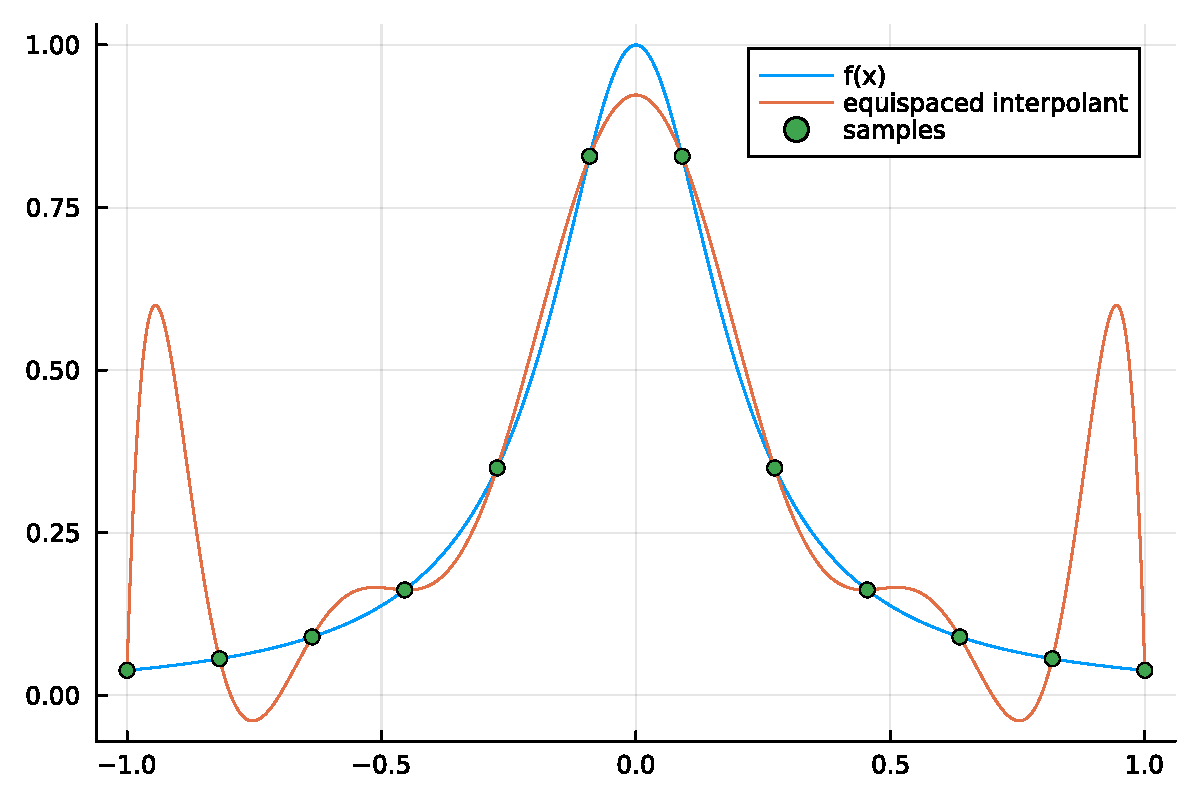
\includegraphics[width=\linewidth]{jl_dOthw0/OP_methods_3_1.pdf}

The oscillations at the ends of the interval become larger as we increase $n$:


\begin{lstlisting}
(*@\HLJLn{n}@*) (*@\HLJLoB{=}@*) (*@\HLJLni{51}@*)
(*@\HLJLn{nodes}@*) (*@\HLJLoB{=}@*) (*@\HLJLnf{range}@*)(*@\HLJLp{(}@*)(*@\HLJLoB{-}@*)(*@\HLJLni{1}@*)(*@\HLJLp{,}@*)(*@\HLJLn{stop}@*)(*@\HLJLoB{=}@*)(*@\HLJLni{1}@*)(*@\HLJLp{,}@*)(*@\HLJLn{length}@*)(*@\HLJLoB{=}@*)(*@\HLJLn{n}@*)(*@\HLJLoB{+}@*)(*@\HLJLni{1}@*)(*@\HLJLp{)}@*)  
(*@\HLJLn{xx}@*) (*@\HLJLoB{=}@*) (*@\HLJLnf{range}@*)(*@\HLJLp{(}@*)(*@\HLJLoB{-}@*)(*@\HLJLni{1}@*)(*@\HLJLp{,}@*)(*@\HLJLni{1}@*)(*@\HLJLp{;}@*)(*@\HLJLn{length}@*)(*@\HLJLoB{=}@*)(*@\HLJLni{501}@*)(*@\HLJLp{)}@*)  (*@\HLJLcs{{\#}}@*) (*@\HLJLcs{plotting}@*) (*@\HLJLcs{grid}@*)
(*@\HLJLn{p}@*) (*@\HLJLoB{=}@*) (*@\HLJLnf{equi{\_}interp}@*)(*@\HLJLp{(}@*)(*@\HLJLn{f}@*)(*@\HLJLp{,}@*)(*@\HLJLn{n}@*)(*@\HLJLp{)}@*) 
(*@\HLJLnf{plot}@*)(*@\HLJLp{(}@*)(*@\HLJLn{xx}@*)(*@\HLJLp{,}@*)(*@\HLJLn{f}@*)(*@\HLJLoB{.}@*)(*@\HLJLp{(}@*)(*@\HLJLn{xx}@*)(*@\HLJLp{);}@*)(*@\HLJLn{label}@*)(*@\HLJLoB{=}@*)(*@\HLJLs{"{}f(x)"{}}@*)(*@\HLJLp{,}@*)(*@\HLJLn{ylims}@*)(*@\HLJLoB{=}@*)(*@\HLJLp{(}@*)(*@\HLJLoB{-}@*)(*@\HLJLni{5}@*)(*@\HLJLp{,}@*)(*@\HLJLni{5}@*)(*@\HLJLp{))}@*)
(*@\HLJLnf{plot!}@*)(*@\HLJLp{(}@*)(*@\HLJLn{xx}@*)(*@\HLJLp{,}@*)(*@\HLJLn{p}@*)(*@\HLJLoB{.}@*)(*@\HLJLp{(}@*)(*@\HLJLn{xx}@*)(*@\HLJLp{);}@*)(*@\HLJLn{label}@*)(*@\HLJLoB{=}@*)(*@\HLJLs{"{}equispaced}@*) (*@\HLJLs{interpolant"{}}@*)(*@\HLJLp{)}@*)
(*@\HLJLnf{scatter!}@*)(*@\HLJLp{(}@*)(*@\HLJLn{nodes}@*)(*@\HLJLp{,}@*)(*@\HLJLn{p}@*)(*@\HLJLoB{.}@*)(*@\HLJLp{(}@*)(*@\HLJLn{nodes}@*)(*@\HLJLp{);}@*)(*@\HLJLn{label}@*)(*@\HLJLoB{=}@*)(*@\HLJLs{"{}samples"{}}@*)(*@\HLJLp{)}@*)
\end{lstlisting}

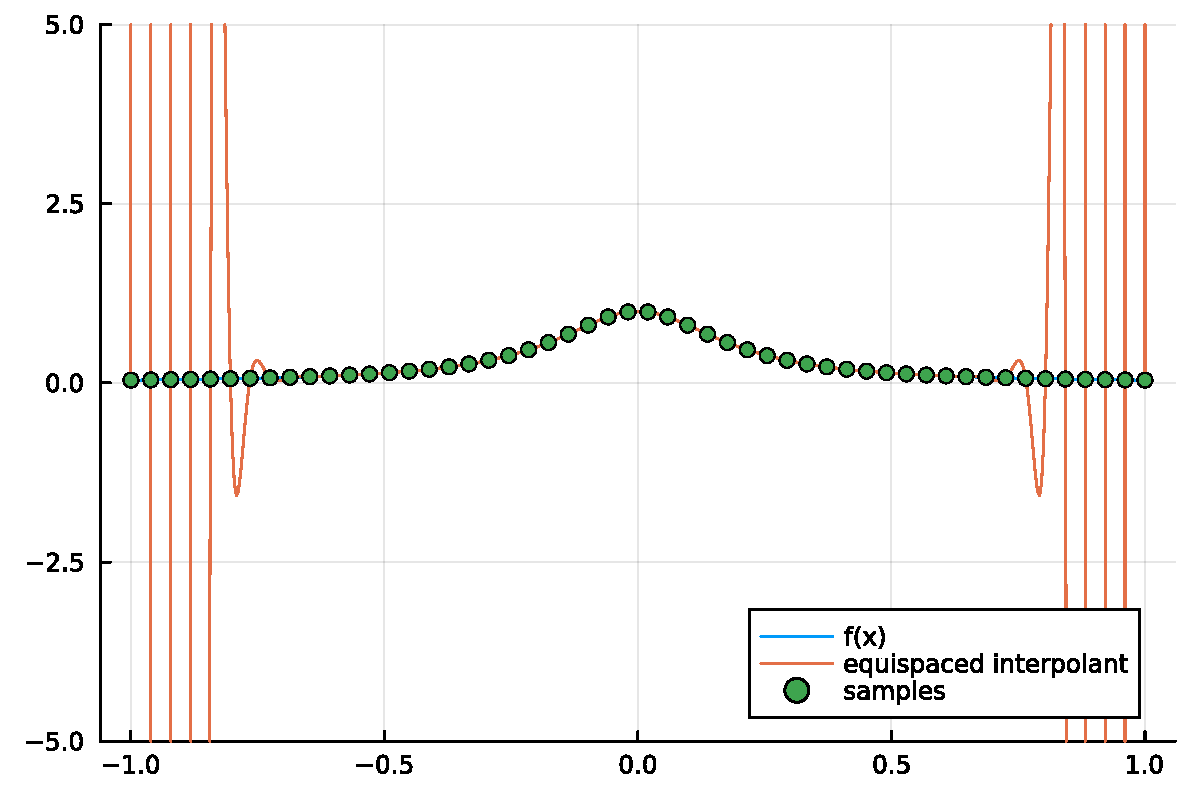
\includegraphics[width=\linewidth]{jl_dOthw0/OP_methods_4_1.pdf}

These oscillations of the interpolant through equally spaced nodes is known as the \emph{Runge phenomenon}. Equally spaced interpolation nodes is clearly not a good choice for polynomial interpolation.  Maybe the oscillations at the endpoints can be suppressed if we choose nodes that are clustered at the ends of the interval?


\begin{lstlisting}
(*@\HLJLn{n}@*) (*@\HLJLoB{=}@*) (*@\HLJLni{11}@*)
(*@\HLJLn{S}@*) (*@\HLJLoB{=}@*) (*@\HLJLnf{Chebyshev}@*)(*@\HLJLp{()}@*)
(*@\HLJLn{p\ensuremath{\_n}}@*) (*@\HLJLoB{=}@*) (*@\HLJLnf{Fun}@*)(*@\HLJLp{(}@*)(*@\HLJLn{f}@*)(*@\HLJLp{,}@*)(*@\HLJLn{S}@*)(*@\HLJLp{,}@*)(*@\HLJLn{n}@*)(*@\HLJLoB{+}@*)(*@\HLJLni{1}@*)(*@\HLJLp{)}@*) 
(*@\HLJLn{xn}@*) (*@\HLJLoB{=}@*) (*@\HLJLnf{points}@*)(*@\HLJLp{(}@*)(*@\HLJLn{S}@*)(*@\HLJLp{,}@*)(*@\HLJLn{n}@*)(*@\HLJLoB{+}@*)(*@\HLJLni{1}@*)(*@\HLJLp{)}@*) 
(*@\HLJLnf{plot}@*)(*@\HLJLp{(}@*)(*@\HLJLn{xx}@*)(*@\HLJLp{,}@*)(*@\HLJLn{f}@*)(*@\HLJLoB{.}@*)(*@\HLJLp{(}@*)(*@\HLJLn{xx}@*)(*@\HLJLp{);}@*)(*@\HLJLn{label}@*)(*@\HLJLoB{=}@*)(*@\HLJLs{"{}f(x)"{}}@*)(*@\HLJLp{)}@*)
(*@\HLJLnf{plot!}@*)(*@\HLJLp{(}@*)(*@\HLJLn{p\ensuremath{\_n}}@*)(*@\HLJLp{;}@*)(*@\HLJLn{label}@*)(*@\HLJLoB{=}@*)(*@\HLJLs{"{}interpolant"{}}@*)(*@\HLJLp{)}@*)
(*@\HLJLnf{scatter!}@*)(*@\HLJLp{(}@*)(*@\HLJLn{xn}@*)(*@\HLJLp{,}@*)(*@\HLJLn{p\ensuremath{\_n}}@*)(*@\HLJLoB{.}@*)(*@\HLJLp{(}@*)(*@\HLJLn{xn}@*)(*@\HLJLp{);}@*)(*@\HLJLn{label}@*)(*@\HLJLoB{=}@*)(*@\HLJLs{"{}samples"{}}@*)(*@\HLJLp{)}@*)
\end{lstlisting}

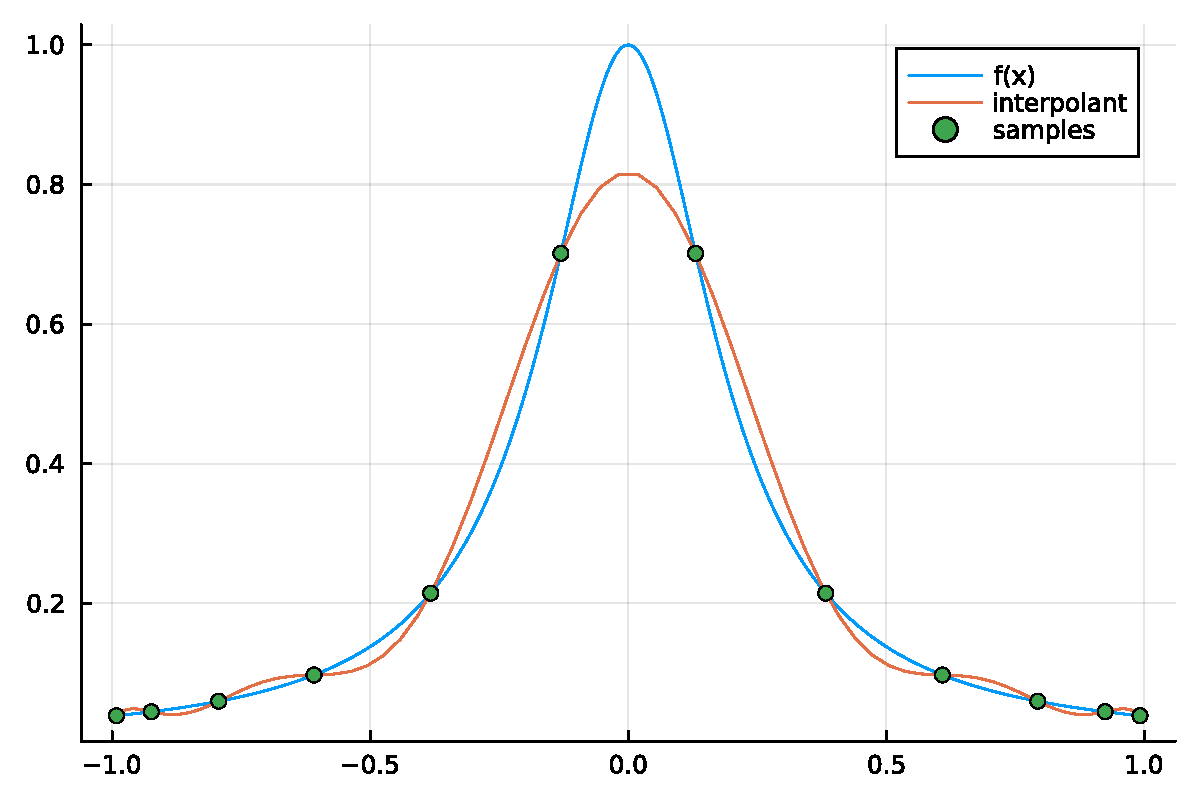
\includegraphics[width=\linewidth]{jl_dOthw0/OP_methods_5_1.pdf}

In the above figure, we interpolated $f(x)$ at the roots of an orthogonal polynomial (OP), which we'll learn about later.  The interpolants at the roots of the OP converge exponentially fast to $f$ on $[-1, 1]$ as $n$ increases.


\begin{lstlisting}
(*@\HLJLn{n}@*) (*@\HLJLoB{=}@*) (*@\HLJLni{31}@*)
(*@\HLJLn{S}@*) (*@\HLJLoB{=}@*) (*@\HLJLnf{Chebyshev}@*)(*@\HLJLp{()}@*)
(*@\HLJLn{p\ensuremath{\_n}}@*) (*@\HLJLoB{=}@*) (*@\HLJLnf{Fun}@*)(*@\HLJLp{(}@*)(*@\HLJLn{f}@*)(*@\HLJLp{,}@*)(*@\HLJLn{S}@*)(*@\HLJLp{,}@*)(*@\HLJLn{n}@*)(*@\HLJLoB{+}@*)(*@\HLJLni{1}@*)(*@\HLJLp{)}@*) 
(*@\HLJLn{xn}@*) (*@\HLJLoB{=}@*) (*@\HLJLnf{points}@*)(*@\HLJLp{(}@*)(*@\HLJLn{S}@*)(*@\HLJLp{,}@*)(*@\HLJLn{n}@*)(*@\HLJLoB{+}@*)(*@\HLJLni{1}@*)(*@\HLJLp{)}@*) 
(*@\HLJLnf{plot}@*)(*@\HLJLp{(}@*)(*@\HLJLn{xx}@*)(*@\HLJLp{,}@*)(*@\HLJLn{f}@*)(*@\HLJLoB{.}@*)(*@\HLJLp{(}@*)(*@\HLJLn{xx}@*)(*@\HLJLp{);}@*)(*@\HLJLn{label}@*)(*@\HLJLoB{=}@*)(*@\HLJLs{"{}f"{}}@*)(*@\HLJLp{)}@*)
(*@\HLJLnf{plot!}@*)(*@\HLJLp{(}@*)(*@\HLJLn{p\ensuremath{\_n}}@*)(*@\HLJLp{;}@*)(*@\HLJLn{label}@*)(*@\HLJLoB{=}@*)(*@\HLJLs{"{}interpolant"{}}@*)(*@\HLJLp{)}@*)
(*@\HLJLnf{scatter!}@*)(*@\HLJLp{(}@*)(*@\HLJLn{xn}@*)(*@\HLJLp{,}@*)(*@\HLJLn{p\ensuremath{\_n}}@*)(*@\HLJLoB{.}@*)(*@\HLJLp{(}@*)(*@\HLJLn{xn}@*)(*@\HLJLp{);}@*)(*@\HLJLn{label}@*)(*@\HLJLoB{=}@*)(*@\HLJLs{"{}samples"{}}@*)(*@\HLJLp{)}@*)
\end{lstlisting}

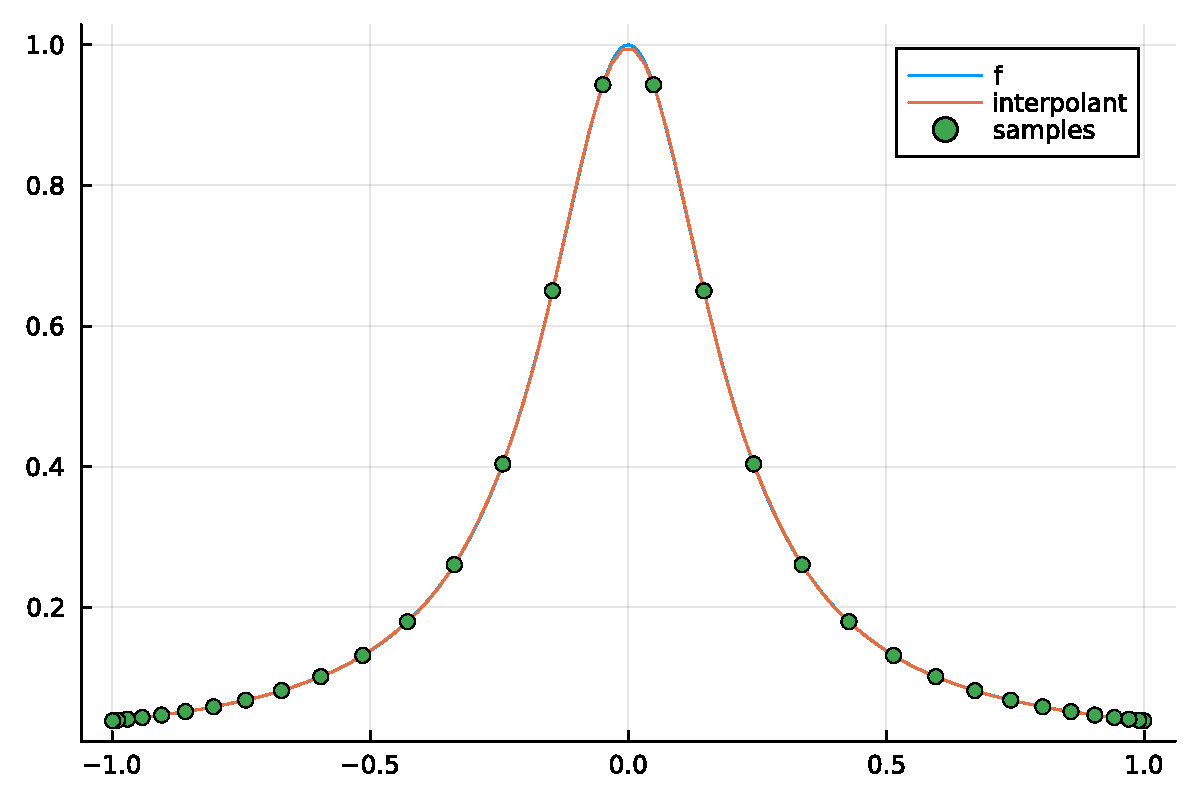
\includegraphics[width=\linewidth]{jl_dOthw0/OP_methods_6_1.pdf}

A deep and quantitative understanding of the reasons why equispaced interpolation failed for the above function and why interpolants through clustered points converged fast is a beautiful and advanced topic that requires tools from complex analysis and potential theory.

We now introduce orthogonal polynomials (OPs). These are \textbf{fundamental} for computational mathematics, with applications in

\begin{itemize}
\item[1. ] Function approximation


\item[2. ] Quadrature (calculating integrals)


\item[3. ] Solving differential equations


\item[4. ] Spectral analysis of Schrödinger operators

\end{itemize}
We will investigate the properties of \emph{general} OPs, in this lecture:

\begin{itemize}
\item[1. ] Definition of orthogonal polynomials


\item[2. ] Three-term recurrence relationships


\item[3. ] Function approximation with orthogonal polynomials


\item[4. ] Construction of orthogonal polynomials via Gram\ensuremath{\endash}Schmidt process

\end{itemize}
In addition to numerics, OPs play a very important role in many mathematical areas including functional analysis, integrable systems, singular integral equations, complex analysis, and random matrix theory.

\begin{itemize}
\item[1. ] General properties of OPs: we define orthogonal polynomials, three-term recurrences and Jacobi operators


\item[2. ] Classical OPs: we define Chebyshev, Legendre, Jacobi, Laguerre, and Hermite.

\end{itemize}
\textbf{Remark (advanced)} Going beyond what we discuss here are many other beautiful properties of orthogonal  polynomials that are useful in computation, analysis, representation theory, quantum mechanics, etc. These include sparse recurrence relationships for derivatives, that they are eigenfunctions of differential equations, their asymptotics,  generating functions, etc. 

\subsection{Definition of orthogonal polynomials}
Let $p_0(x),p_1(x),p_2(x),\ensuremath{\ldots}$ be a sequence of polynomials such that $p_n(x)$ is exactly of degree $n$, that is,

\[
p_n(x) = k_n x^n + O(x^{n-1})
\]
where $k_n \neq 0$.

Let $w(x)$ be a continuous weight function on a (possibly infinite) interval $(a,b)$: that is $w(x) \geq 0$ for all $a < x < b$. This induces an inner product

\[
\langle f,g \rangle := \int_a^b f(x) g(x) w(x) {\rm d}x
\]
We say that $\{p_0, p_1,\ldots\}$ are \emph{orthogonal with respect to the weight $w$} if

\[
\langle p_n,p_m \rangle = 0\qquad \text{ for }\: n \neq m.
\]
Because $w$ is continuous, we have

\[
\| p_n \|^2 = \langle p_n,p_n \rangle > 0 .
\]
Orthogonal polymomials are not unique: we can multiply each $p_n$ by a different nonzero constant $\tilde p_n(x) = c_n p_n(x)$, and $\tilde p_n$ will be orthogonal w.r.t. $w$.  However, if we specify $k_n$, this is sufficient to uniquely define them:

\textbf{Proposition (Uniqueness of OPs I)} Given a non-zero $k_n$, there is a unique polynomial $p_n$ orthogonal w.r.t. $w$ to all lower degree polynomials.

\textbf{Proof} Suppose $r_n(x) = k_n x^n + O(x^{n-1})$ is another  OP w.r.t. $w$. We want to show $p_n - r_n$ is zero. But this is a polynomial of degree $<n$, hence

\[
p_n(x) - r_n(x) = \sum_{k=0}^{n-1} c_k p_k(x)
\]
But we have for $k \leq n-1$

\[
\langle p_k,p_k \rangle c_k = \langle p_n - r_n, p_k \rangle = \langle p_n,p_k \rangle - \langle r_n, p_k\rangle = 0 - 0 = 0
\]
which shows all $c_k$ are zero.

\[
\blacksquare
\]
\textbf{Corollary (Uniqueness of OPs I)} If $q_n$ and $p_n$ are orthogonal w.r.t. $w$ to all lower degree polynomials, then $q_n(x) = C p_n(x)$ for some constant $C$.

\subsubsection{Monic orthogonal polynomials}
If $k_n = 1$, that is,

\[
p_n(x) = x^n + O(x^{n-1})
\]
then we refer to the orthogonal polynomials as monic.

Monic OPs are unique as we have specified $k_n$.

\subsubsection{Orthonormal polynomials}
If  $\| p_n \| = 1$, then we refer to the orthogonal polynomials as orthonormal w.r.t. $w$. We will usually use $q_n$ when they are orthonormal.   Note it's not unique: we can multiply by $\pm 1$ without changing the norm.

\textbf{Remark} The classical OPs are neither monic nor orthonormal (apart from one case). Many people make the mistake of using orthonormal polynomials for computations. But there is a good reason to use classical OPs: their properties result in rational formulae, whereas orthonormal polynomials require square roots. This makes a performance difference.

\subsection{Orthogonal polynomials: definitions and properties}
The set of polynomials of degree $\leq n$ with real coefficients, $\mathbb{P}_n$, is a linear space (or vector space) of dimension $n+1$.  The set of  monomials of degree $\leq n$, $\lbrace 1, x, x^2, \ldots, x^n \rbrace$, is a basis for the space $\mathbb{P}_n$, meaning that all polynomials of degree $\leq n$ can be expressed as linear combinations of monomials.  For example, the Lagrange interpolating polynomial of degree $\leq n$ can be expressed in the monomial basis.  However,  it is more efficient and stable to perform computations in OP bases as oposed to the monomial basis.

\textbf{Definition (graded polynomial basis)} A set of polynomials $\{p_0(x), p_1(x), \ensuremath{\ldots} \}$ is \emph{graded} if $p_n$ is precisely degree $n$: i.e.,

\[
p_n(x) = k_n x^n + k_n^{(n-1)} x^{n-1} + \ensuremath{\cdots} + k_n^{(1)} x + k_n^{(0)}
\]
with $k_n \ensuremath{\ne} 0$.

Note that if the $p_n$ are graded then $\{p_0(x), \ensuremath{\ldots}, p_n(x) \}$ form a basis for all polynomials of degree $n$.  For example, the Lagrange interpolating polynomial can be expressed in any graded polynomial basis.

\textbf{Definition (orthogonal polynomials)} Given an (integrable) \emph{weight} $w(x) > 0$ for $x \ensuremath{\in} (a,b)$, associated with which is the inner product

\[
\ensuremath{\langle}f,g\ensuremath{\rangle} = \ensuremath{\int}_a^b  f(x) g(x) w(x) {\rm d} x
\]
a graded polynomial basis $\{p_0(x), p_1(x), \ensuremath{\ldots} \}$ is a set of \emph{orthogonal polynomials (OPs)} if

\[
\ensuremath{\langle}p_n,p_m\ensuremath{\rangle} = 0
\]
whenever $n \ensuremath{\ne} m$.

Note in the above

\[
h_n := \ensuremath{\langle}p_n,p_n\ensuremath{\rangle} = \|p_n\|^2 = \ensuremath{\int}_a^b  p_n(x)^2 w(x) {\rm d} x > 0.
\]
Multiplying any orthogonal polynomial by a constant necessarily is also an orthogonal polynomial. We have two standard normalisations:

\textbf{Definition (orthonormal polynomials)} A set of orthogonal polynomials $\{q_0(x), q_1(x), \ensuremath{\ldots} \}$ are \emph{orthonormal} if $\|q_n\| = 1$.

\textbf{Definition (monic orthogonal polynomials)} A set of orthogonal polynomials $\{p_0(x), p_1(x), \ensuremath{\ldots} \}$ are \emph{monic} if $k_n = 1$.

\textbf{Proposition (existence)} Given a weight $w(x)$, monic orthogonal polynomials exist.

\textbf{Proof}

Existence follows immediately from the Gram\ensuremath{\endash}Schmidt procedure. That is, define $p_0(x) := 1$ and

\[
p_n(x) := x^n - \ensuremath{\sum}_{k=0}^{n-1} {\ensuremath{\langle}x^n,p_k\ensuremath{\rangle} \over \|p_k\|^2} p_k(x)
\]
\[
\blacksquare
\]
\subsection{Function approximation with orthogonal polynomials}
A basic usage of orthogonal polynomials is for polynomial approximation. Suppose $f(x)$ is a degree $n-1$ polynomial. Since $\{p_0(x),\ldots,p_{n-1}(x)\}$ span all degree $n-1$ polynomials, we know that

\[
f(x) = \sum_{k=0}^{n-1} f_k p_k(x)
\]
where

\[
f_k = {\langle f, p_k \rangle \over \langle p_k,p_k \rangle}
\]
Sometimes, we want to incorporate the weight into the approximation. This is typically one of two forms, depending on the application:

\[
f(x) = w(x) \sum_{k=0}^\infty f_k p_k(x)
\]
or

\[
        f(x) = \sqrt{w(x)} \sum_{k=0}^\infty f_k p_k(x)
\]
The $w(x)p_k(x)$ or $\sqrt{w(x)}p_k(x)$ are called weighted polynomials.

We are primarly concerned with the usage of orthogonal polynomials in approximating functions. First we observe the following:

\textbf{Proposition (expansion)} If $r(x)$ is a degree $n$ polynomial, $\{p_n\}$ are orthogonal and $\{q_n\}$ are orthonormal then


\begin{align*}
r(x) &= \ensuremath{\sum}_{k=0}^n {\ensuremath{\langle}p_k,r\ensuremath{\rangle} \over \|p_k\|^2} p_k(x) \\
     &    = \ensuremath{\sum}_{k=0}^n \ensuremath{\langle}q_k,r\ensuremath{\rangle} q_k(x)
\end{align*}
\textbf{Proof} Because $\{p_0,\ensuremath{\ldots},p_n \}$ are a basis of polynomials we can write

\[
r(x) = \ensuremath{\sum}_{k=0}^n r_k p_k(x)
\]
for constants $r_k \ensuremath{\in} \ensuremath{\bbR}$. By linearity we have

\[
\ensuremath{\langle}p_m,r\ensuremath{\rangle} = \ensuremath{\sum}_{k=0}^n r_k \ensuremath{\langle}p_m,p_k\ensuremath{\rangle}= r_m \ensuremath{\langle}p_m,p_m\ensuremath{\rangle}
\]
for $m = 0, \ldots, n$. $\blacksquare$

\textbf{Corollary (zero inner product)} If a degree $n$ polynomial $r$ satisfies

\[
0 = \ensuremath{\langle}p_0,r\ensuremath{\rangle} = \ensuremath{\ldots} = \ensuremath{\langle}p_n,r\ensuremath{\rangle}
\]
then $r = 0$.

\textbf{Corollary (uniqueness)} Monic orthogonal polynomials are unique.

\textbf{Proof} If $\widetilde{p}_n(x)$ and $p_n(x)$ are both monic orthogonal polynomials then $r(x) = \widetilde{p}_n(x) - p_n(x)$ is degree $n-1$ but satisfies

\[
\ensuremath{\langle}r, p_k\ensuremath{\rangle} = \ensuremath{\langle}\widetilde{p}_n, p_k\ensuremath{\rangle} - \ensuremath{\langle}p_n, p_k\ensuremath{\rangle} = 0
\]
for $k = 0,\ensuremath{\ldots},{n-1}$. Note $\ensuremath{\langle}\widetilde{p}_n, p_k\ensuremath{\rangle} = 0$ can be seen by expanding

\[
p_k(x) = \ensuremath{\sum}_{j=0}^k c_j \widetilde{p}_j(x).
\]
\[
\blacksquare
\]
OPs are uniquely defined (up to a constant) by the property that they are orthogonal to all lower degree polynomials.

\textbf{Proposition (orthogonal to lower degree)} Given a weight $w(x)$,  a polynomial $p$ of precisely degree $n$ satisfies

\[
\ensuremath{\langle}p,r\ensuremath{\rangle} = 0
\]
for all degree $m < n$ polynomials $r$ if and only if $p(x) = c p_n(x)$ where $p_n(x)$ are the monic orthogonal polynomials. Therefore an orthogonal polynomial is uniquely defined by $k_n$.

\textbf{Proof} ($\Leftarrow$) As $\{p_0,\ensuremath{\ldots},p_n\}$ are a basis of all polynomials of degree $n$, we can write

\[
r(x) = \ensuremath{\sum}_{k=0}^m a_k p_k(x)
\]
Thus by linearity of inner products we have

\[
\ensuremath{\langle}cp_n,\ensuremath{\sum}_{k=0}^m a_k p_k\ensuremath{\rangle} = \ensuremath{\sum}_{k=0}^m ca_k \ensuremath{\langle}p_n, p_k\ensuremath{\rangle} = 0.
\]
($\Rightarrow$) Now for

\[
p(x) = c x^n + O(x^{n-1})
\]
consider $p(x) - c p_n(x)$ which is of degree $n-1$. It satisfies for $k \ensuremath{\leq} n-1$

\[
\ensuremath{\langle}p_k, p - c p_n\ensuremath{\rangle} = \ensuremath{\langle}p_k, p\ensuremath{\rangle} - c \ensuremath{\langle}p_k, p_n\ensuremath{\rangle} = 0.
\]
Thus it is zero, i.e., $p(x) = c p_n(x)$.

\[
\blacksquare
\]
A consequence of this is that orthonormal polynomials are always a constant multiple of orthogonal polynomials.

\subsection{Jacobi matrices and three-term recurrences for general orthogonal polynomials}
\subsubsection{Three-term recurrence relationships}
A central theme: if you know the Jacobi matrix / three-term recurrence, you know the polynomials. This is the \textbf{best} way to evaluate expansions in orthogonal polynomials: even for cases where we have explicit formulae (e.g. Chebyshev polynomials $T_n(x) = \cos n \arccos x$), using the recurrence avoids evaluating trigonometric functions.

Every family of orthogonal polynomials has a three-term recurrence relationship:

\textbf{Theorem (three-term recurrence)} Suppose $\{p_n(x)\}$ are a family of orthogonal polynomials w.r.t. a weight $w(x)$. Then there exists constants $a_n$, $b_n \neq 0$ and $c_n$ such that


\begin{align*}
x p_0(x) = a_0 p_0(x) + b_0 p_1(x) \\
x p_n(x) = c_n p_{n-1}(x) + a_n p_n(x) + b_n p_{n+1}(x)
\end{align*}
\textbf{Proof} The first part follows since $p_0(x)$ and $p_1(x)$ span all degree 1 polynomials.

The second part follows essentially because multiplication by $x$ is "self-adjoint", that is,

\[
\langle x f, g\rangle = \int_a^b x f(x) g(x) w(x) {\rm d}x = \langle f, x g \rangle
\]
Therefore, if $f_m$ is a degree $m < n-1$ polynomial, we have

\[
\langle x p_n, f_m\rangle = \langle p_n, x f_m\rangle = 0.
\]
In particular, if we write

\[
x p_n(x) = \sum_{k=0}^{n+1} C_k p_k(x)
\]
then

\[
C_k = {\langle x p_n, p_k\rangle \over \| p_k\|^2} = 0
\]
if $k < n-1$. $\blacksquare$

Monic polynomials clearly have $b_n = 1$.  Orthonormal polynomials have an even simpler form:

\textbf{Theorem (orthonormal three-term recurrence)} Suppose $\{q_n(x)\}$ are a family of orthonormal polynomials w.r.t. a weight $w(x)$. Then there exists constants $a_n$ and $b_n$ such that


\begin{align*}
x q_0(x) = a_0 q_0(x)  + b_0 q_1(x)\\
x q_n(x) = b_{n-1} q_{n-1}(x) + a_n q_n(x) + b_{n} q_{n+1}(x)
\end{align*}
\textbf{Proof} Follows again by self-adjointness of multiplication by $x$:

\[
c_n = \langle x q_n, q_{n-1}\rangle = \langle q_n, x q_{n-1}\rangle = \langle x q_{n-1}, q_n\rangle = b_{n-1}
\]
\[
\blacksquare
\]
\textbf{Corollary (symmetric three-term recurrence implies orthonormality)} Suppose $\{p_n(x)\}$ are a family of orthogonal polynomials w.r.t. a weight $w(x)$ such that


\begin{align*}
x p_0(x) = a_0 p_0(x)  + b_0 p_1(x)\\
x p_n(x) = b_{n-1} p_{n-1}(x) + a_n p_n(x) + b_{n} p_{n+1}(x)
\end{align*}
with $b_n \neq 0$. Suppose further that $\| p_0 \| = 1$. Then $p_n$ must be orthonormal.

\textbf{Proof} This follows from

\[
b_n = {\langle x p_n,p_{n+1} \rangle \over \| p_{n+1}\|^2} = {\langle x p_{n+1}, p_n\rangle \over \|p_{n+1}\|^2} = b_n   {\|p_n\|^2 \over \|p_{n+1}\|^2 }
\]
which implies

\[
\|p_{n+1}\|^2 = \|p_n\|^2 = \cdots = \|p_0\|^2 = 1
\]
\[
\blacksquare
\]
\textbf{Remark} We can scale $w(x)$ by a constant without changing the orthogonality properties, hence we can make $\|p_0\| = 1$ by changing the weight.

\textbf{Remark} This is beyond the scope of this course, but satisfying a three-term recurrence like this such that coefficients are bounded with $p_0(x) = 1$ is sufficient to show that there exists a $w(x)$ (or more accurately, a Borel measure) such that $p_n(x)$ are orthogonal w.r.t. $w$. The relationship between the coefficients $a_n,b_n$ and the $w(x)$ is an object of study in spectral theory, particularly when the coefficients are periodic, quasi-periodic or random.

\subsubsection{3-term recurrence}
The most \emph{fundamental} property of orthogonal polynomials is their three-term recurrence.

\textbf{Theorem (3-term recurrence, 2nd form)} If $\{p_n\}$ are OPs then there exist real constants $a_n, b_n \ensuremath{\ne}0,c_{n-1} \ensuremath{\ne}0$ such that


\begin{align*}
x p_0(x) &= a_0 p_0(x) + b_0 p_1(x)  \\
x p_n(x) &= c_{n-1} p_{n-1}(x) + a_n p_n(x) + b_n p_{n+1}(x)
\end{align*}
\textbf{Proof} The $n=0$ case is immediate since $\{p_0,p_1\}$ are a basis of degree 1 polynomials. The $n >0$ case follows from

\[
\ensuremath{\langle}x p_n, p_k\ensuremath{\rangle} = \ensuremath{\langle} p_n, xp_k\ensuremath{\rangle} = 0
\]
for $k < n-1$ as $x p_k$ is of degree $k+1 < n$.

Note that

\[
b_n = {\ensuremath{\langle}p_{n+1}, x p_n\ensuremath{\rangle} \over \|p_{n+1} \|^2} \ensuremath{\ne} 0
\]
since $x p_n = k_n x^{n+1} + O(x^n)$ is precisely degree $n$. Further,

\[
c_{n-1} = {\ensuremath{\langle}p_{n-1}, x p_n\ensuremath{\rangle} \over \|p_{n-1}\|^2 } =
{\ensuremath{\langle}p_n, x p_{n-1}\ensuremath{\rangle}  \over \|p_{n-1}\|^2 } =  b_{n-1}{\|p_n\|^2  \over \|p_{n-1}\|^2 } \ensuremath{\ne} 0.
\]
\[
\blacksquare
\]
Clearly if $p_n$ is monic then so is $x p_n$ which leads to the following:

\textbf{Corollary (monic 3-term recurrence)} If $\{p_n\}$ are monic then $b_n =  1$.

\textbf{Example} What are the  monic OPs $p_0(x),\ensuremath{\ldots},p_3(x)$ with respect to $w(x) = 1$ on $[0,1]$? We can construct these using Gram\ensuremath{\endash}Schmidt, but exploiting the 3-term recurrence to reduce the computational cost. We have $p_0(x) = 1$, which we see is orthogonal:

\[
\|p_0\|^2 = \ensuremath{\langle}p_0,p_0\ensuremath{\rangle} = \ensuremath{\int}_0^1 {\rm d x} = 1.
\]
We know from the 3-term recurrence that

\[
x p_0(x) = a_0 p_0(x) +  p_1(x)
\]
where

\[
a_0 = {\ensuremath{\langle}p_0,x p_0\ensuremath{\rangle}  \over \|p_0\|^2} = \ensuremath{\int}_0^1 x {\rm d} x = 1/2.
\]
Thus


\begin{align*}
p_1(x) = x p_0(x) - a_0 p_0(x) = x-1/2 \\
\|p_1\|^2 = \ensuremath{\int}_0^1 (x^2 - x + 1/4) {\rm d} x = 1/12
\end{align*}
From

\[
x p_1(x) = c_0 p_0(x) + a_1 p_1(x) +  p_2(x)
\]
we have


\begin{align*}
c_0 &= {\ensuremath{\langle}p_0,x p_1\ensuremath{\rangle}  \over \|p_0\|^2} = \ensuremath{\int}_0^1 (x^2 - x/2) {\rm d} x = 1/12 \\
a_1 &= {\ensuremath{\langle}p_1,x p_1\ensuremath{\rangle}  \over \|p_1\|^2} = 12 \ensuremath{\int}_0^1 (x^3 - x^2 + x/4) {\rm d} x = 1/2 \\
p_2(x) &= x p_1(x) - c_0 - a_1 p_1(x) = x^2 - x + 1/6 \\
\|p_2\|^2 &= \int_0^1 (x^4 - 2x^3 + 4x^2/3 - x/3 + 1/36) {\rm d} x = {1 \over 180}
\end{align*}
Finally, from

\[
x p_2(x) = c_1 p_1(x) + a_2 p_2(x) +  p_3(x)
\]
we have


\begin{align*}
c_1 &= {\ensuremath{\langle}p_1,x p_2\ensuremath{\rangle}  \over \|p_1\|^2} = 12 \ensuremath{\int}_0^1 (x^4 - 3x^3/2 +2x^2/3 -x/12)  {\rm d} x = 1/15 \\
a_2 &= {\ensuremath{\langle}p_2,x p_2\ensuremath{\rangle}  \over \|p_2\|^2} = 180 \ensuremath{\int}_0^1 (x^5 - 2x^4 +4x^3/3 - x^2/3 + x/36) {\rm d} x = 1/2 \\
p_3(x) &= x p_2(x) - c_1 p_1(x)- a_2 p_2(x) = x^3 - x^2 + x/6 - x/15 + 1/30 -x^2/2 + x/2 - 1/12 \\
&= x^3 - 3x^2/2 + 3x/5 -1/20
\end{align*}
\subsection{Jacobi matrices and multiplication by $x$}
We can rewrite the three-term recurrence as

\[
x \begin{pmatrix} p_0(x) \cr p_1(x) \cr p_2(x) \cr \vdots \end{pmatrix} = J\begin{pmatrix} p_0(x) \cr p_1(x) \cr p_2(x) \cr \vdots \end{pmatrix}
\]
where $J$ is a Jacobi matrix, an infinite-dimensional tridiagonal matrix:

\[
J = \begin{pmatrix}
a_0 & b_0 \cr
c_1 & a_1 & b_1 \cr
& c_2 & a_2 & b_2 \cr
&& c_3 & a_3 & \ddots \cr
&&&\ddots & \ddots
\end{pmatrix}
\]
When the polynomials are monic, we have $1$ on the superdiagonal.  When we have an orthonormal basis, then $J$ is symmetric:

\[
J = \begin{pmatrix}
a_0 & b_0 \cr
b_0 & a_1 & b_1 \cr
& b_1 & a_2 & b_2 \cr
&& b_2 & a_3 & \ddots \cr
&&&\ddots & \ddots
\end{pmatrix}
\]
Given a polynomial expansion, $J$ tells us how to multiply by $x$ in coefficient space, that is, if

\[
f(x) = \sum_{k=0}^\infty f_k p_k(x) =   (p_0(x) ,  p_1(x) , \ldots ) \begin{pmatrix}f_0\\ f_1\\f_2\\\vdots\end{pmatrix}
\]
then (provided the relevant sums converge absolutely and uniformly)

\[
x f(x) = x (p_0(x) ,  p_1(x) , \ldots ) \begin{pmatrix}f_0\\ f_1\\f_2\\\vdots\end{pmatrix} =
    \left(J \begin{pmatrix} p_0(x) \cr p_1(x) \cr p_2(x) \cr \vdots \end{pmatrix}\right)^\top  \begin{pmatrix}f_0\\ f_1\\f_2\\\vdots\end{pmatrix} = (p_0(x) ,  p_1(x) , \ldots ) X \begin{pmatrix}f_0\\ f_1\\f_2\\\vdots\end{pmatrix}
\]
where $X := J^\top$.

\subsubsection{Jacobi matrix}
The three-term recurrence can also be interpreted as a matrix known as the Jacobi matrix:

\textbf{Corollary (Jacobi matrix)} For

\[
P(x) := [p_0(x) | p_1(x) | \ensuremath{\cdots}]
\]
then we have

\[
x P(x) = P(x) \underbrace{\begin{bmatrix} a_0 & c_0 \\
                                                        b_0 & a_1 & c_1\\
                                                        & b_1 & a_2 & \ensuremath{\ddots} \\
                                                        && \ensuremath{\ddots} & \ensuremath{\ddots}
                                                        \end{bmatrix}}_X
\]
More generally, for any polynomial $a(x)$ we have

\[
a(x) P(x) = P(x) a(X).
\]
For the special cases of orthonormal and monic polynomials we have extra structure:

\textbf{Corollary (orthonormal 3-term recurrence)} If $\{q_n\}$ are orthonormal then its recurrence coefficients satisfy $c_n = b_n$. That is, the Jacobi matrix is symmetric:

\[
X = \begin{bmatrix} a_0 & b_0 \\
                                                        b_0 & a_1 & b_1\\
                                                        & b_1 & a_2 & \ensuremath{\ddots} \\
                                                        && \ensuremath{\ddots} & \ensuremath{\ddots}
                                                        \end{bmatrix}
\]
\textbf{Proof}

\[
b_n = \ensuremath{\langle}x q_n, q_{n+1}\ensuremath{\rangle} = \ensuremath{\langle}q_n, x q_{n+1}\ensuremath{\rangle} = c_{n-1}.
\]
\[
\blacksquare
\]
\textbf{Remark} Typically the Jacobi matrix is the transpose $J := X^\ensuremath{\top}$. If the basis are orthonormal then $X$ is symmetric and they are the same.

\textbf{Remark (advanced)} If you are worried about multiplication of infinite matrices/vectors note it is well-defined by the standard definition because it is banded. It can also be defined in terms of functional analysis where one considers these as linear operators (functions of functions) between vector spaces.

\textbf{Remark (advanced)} Every integrable weight generates a family of orthonormal polynomials, which in turn generates a symmetric Jacobi matrix. There is a "Spectral Theorem for Jacobi matrices" that says one can go the other way: every tridiagonal symmetric matrix with bounded entries is a Jacobi matrix for some integrable weight with compact support. This is an example of what \href{https://en.wikipedia.org/wiki/Barry_Simon}{Barry Simon} calls a "Gem of spectral theory", that is.

\textbf{Example (uniform weight Jacobi matrix)} Consider the monic orthogonal polynomials $p_0(x),p_1(x),\ensuremath{\ldots},p_3(x)$ for $w(x) = 1$ on $[0,1]$ constructed above. We can write the 3-term recurrence coefficients we have computed above as the Jacobi matrix:

\[
x [p_0(x)| p_1(x)| \ensuremath{\cdots}] = [p_0(x)| p_1(x)| \ensuremath{\cdots}] \underbrace{\begin{bmatrix} 1/2 & 1/12 \\
                                                            1 & 1/2 & 1/15 \\
                                                            & 1 & 1/2 & \ensuremath{\ddots} \\
                                                            & & \ensuremath{\ddots} & \ensuremath{\ddots} \end{bmatrix}}_X
\]
We can compute the orthonormal polynomials, using

\[
\|p_3\|^2 = \int_0^1 (x^6 - 3x^5 + 69x^4/20 -19x^3/10 + 51x^2/100 - 3x/50 + 1/400) {\rm d}x = {1 \over 2800}
\]
as:


\begin{align*}
q_0(x) &= p_0(x) \\
q_1(x) &= \sqrt{12} p_1(x)= \sqrt{3} (2  x - 1) \\
q_2(x) &= \sqrt{180} p_2(x) = \sqrt{5} (6x^2 - 6x + 1) \\
q_3(x) &= \sqrt{2800} p_3(x) = \sqrt{7} (20x^3-30x^2 + 12x - 1)
\end{align*}
which have the Jacobi matrix


\begin{align*}
x [q_0(x)| q_1(x)| \ensuremath{\cdots}] &= x [p_0(x)| p_1(x)| \ensuremath{\cdots}] \underbrace{\begin{bmatrix} 1 \\ & 2\sqrt{3} \\ && 6 \sqrt{5} \\ &&& 20 \sqrt{7} \\
&&&& \ensuremath{\ddots}
\end{bmatrix}}_D \\
&= [q_0(x)| q_1(x)| \ensuremath{\cdots}] D^{-1} X D = 
     \begin{bmatrix} 1/2 & 1/\sqrt{12} \\
                    1/\sqrt{12} & 1/2 &  1/\sqrt{15} \\
                    & 1/\sqrt{15} & 1/2 & \ensuremath{\ddots} \\
                    & \ensuremath{\ddots} & \ensuremath{\ddots} \end{bmatrix}
\end{align*}
which is indeed symmetric. The problem sheet explores a more elegant way of doing this.

\textbf{Example (expansion)} Consider expanding a low degree polynomial like $f(x) = x^2$ in $p_n(x)$. We have

\[
\ensuremath{\langle}p_0, f\ensuremath{\rangle} = \ensuremath{\int}_0^1 x^2 {\rm d} x = 1/3
\ensuremath{\langle}p_1, f\ensuremath{\rangle} = \ensuremath{\int}_0^1 x^2 (x - 1/2) {\rm d} x = 1/12
\ensuremath{\langle}p_2, f\ensuremath{\rangle} = \ensuremath{\int}_0^1 x^2 (x^2 - x + 1/6) {\rm d} x = 1/180
\]
Thus we have:

\[
f(x) = {p_0(x) \over 3} + p_1(x) + p_2(x) = [p_0(x) | p_1(x) | p_2(x) | \ensuremath{\cdots}] \begin{bmatrix} 1/3 \\ 1 \\ 1 \\ 0 \\ \ensuremath{\vdots} \end{bmatrix}
\]
We multiply (using that $b_2 = 1$ for monic OPs) to deduce:


\begin{align*}
x f(x) &= x[p_0(x) | p_1(x) | p_2(x) | \ensuremath{\cdots}] \begin{bmatrix} 1/3 \\ 1 \\ 1 \\ 0 \\ \ensuremath{\vdots} \end{bmatrix} \\
&= [p_0(x) | p_1(x) | p_2(x) | \ensuremath{\cdots}] X \begin{bmatrix} 1/3 \\ 1 \\ 1 \\ 0 \\ \ensuremath{\vdots} \end{bmatrix}
= [p_0(x) | p_1(x) | p_2(x) | \ensuremath{\cdots}]  \begin{bmatrix} 1/4 \\ 9/10 \\ 3/2 \\ 1 \\ 0 \\ \ensuremath{\vdots} \end{bmatrix} \\
&= {p_0(x) \over 4} + {9 p_1(x) \over 10} + {3 p_2(x) \over 2} + p_3(x)
\end{align*}
\subsubsection{Evaluating polynomials}
We can use the three-term recurrence to construct the polynomials. One way to express this is in the language of linear algebra. Suppose we are given $p_0(x) = k_0$ (where $k_0 = 1$ is pretty much always the case in practice). This can be written in matrix form as

\[
(1,0,0,0,0,\ldots) \begin{pmatrix} p_0(x) \cr p_1(x) \cr p_2(x) \cr \vdots \end{pmatrix} = k_0
\]
We can combine this with the Jacobi operator to get

\[
\underbrace{\begin{pmatrix}
1 \\
a_0-x & b_0 \\
c_1 & a_1-x & b_1 \\
& c_2 & a_2-x & b_2 \cr
&& c_3 & a_3-x & b_3 \cr
&&&\ddots & \ddots & \ddots
\end{pmatrix}}_{L_x} \begin{pmatrix} p_0(x) \cr p_1(x) \cr p_2(x) \cr \vdots \end{pmatrix} = \begin{pmatrix} k_0\cr 0 \cr 0 \cr \vdots \end{pmatrix}
\]
For $x$ fixed, this is a lower triangular system, that is, the polynomials equal

\[
k_0 L_x^{-1} \mathbf{ e}_0
\]
This  can be solved  via forward recurrence:


\begin{align*}
    p_0(x) &= k_0 \\
    p_1(x) &= {(x-a_0) p_0(x) \over b_0}\\
    p_2(x) &= {(x-a_1) p_0(x) - c_1 p_0(x) \over b_1}\\
    p_3(x) &= {(x-a_2) p_1(x) - c_2 p_1(x) \over b_2}\\
    &\vdots
\end{align*}
We can use this to evaluate functions as well:

\[
f(x) = (p_0(x),p_1(x),\ldots) \begin{pmatrix}f_0 \\ f_1\\ \vdots \end{pmatrix} =
k_0 \mathbf{e}_0^\top L_x^{-\top}  \begin{pmatrix}f_0 \\ f_1\\ \vdots \end{pmatrix}
\]
when $f$ is a degree $n-1$ polynomial, this becomes a problem of inverting an upper triangular matrix, that is, we want to solve the $n \times n$ system

\[
\underbrace{\begin{pmatrix}
1 & a_0-x & c_1 \\
& b_0 & a_1-x & c_2  \\
& & b_1 & a_2-x & \ddots  \\
& &     & b_2 & \ddots & c_{n-2} \\
&&&&\ddots & a_{n-2}-x \\
&&&&& b_{n-2}
\end{pmatrix}}_{L_x^\top} \begin{pmatrix} \gamma_0 \\\vdots\\ \gamma_{n-1} \end{pmatrix}
\]
so that $f(x)/k_0 = \gamma_0$. We can solve this  via back-substitution:


\begin{align*}
\gamma_{n-1} &= {f_{n-1} \over b_{n-2}} \\
\gamma_{n-2} &= {f_{n-2} - (a_{n-2}-x) \gamma_{n-1} \over b_{n-3}} \\
\gamma_{n-3} &= {f_{n-3} - (a_{n-3}-x) \gamma_{n-2} - c_{n-2} \gamma_{n-1} \over b_{n-4}} \\
& \vdots \\
\gamma_1 &= {f_1 - (a_1-x) \gamma_2 - c_2 \gamma_3 \over b_0} \\
\gamma_0 &= f_0 - (a_0-x) \gamma_1 - c_1 \gamma_2
\end{align*}
We give examples of these algorithms applied to Chebyshev polynomials in the next lecture.

\subsection{Gram\ensuremath{\endash}Schmidt algorithm}
In general we don't have nice formulae for OPs but we can always construct them via the Gram\ensuremath{\endash}Schmidt process:

\textbf{Proposition (Gram\ensuremath{\endash}Schmidt)} Define


\begin{align*}
p_0(x) = 1 \\
q_0(x) = {1 \over \|p_0\|}\\
p_{n+1}(x) = x q_n(x) - \sum_{k=0}^n \langle x q_n, q_k\rangle q_k(x)\\
q_{n+1}(x) = {p_{n+1}(x) \over \|p_{n+1}\|}
\end{align*}
Then $q_0(x), q_1(x), \ldots$ are orthonormal w.r.t. $w$.

\textbf{Proof} By linearity we have

\[
\langle p_{n+1}, q_j\rangle = \left\langle x q_n - \sum_{k=0}^n {\langle x q_n, q_k\rangle} q_k, q_j\right\rangle = \langle x q_n, q_j\rangle - \langle x q_n, q_j\rangle \langle q_j,q_j\rangle = 0
\]
Thus $p_{n+1}$ is orthogonal to all lower degree polynomials. So is $q_{n+1}$, since it is a constant multiple of $p_{n+1}$.

\[
\blacksquare
\]
Let's make our own family of OPs:


\begin{lstlisting}
(*@\HLJLk{using}@*) (*@\HLJLn{ApproxFun}@*)(*@\HLJLp{,}@*) (*@\HLJLn{Plots}@*)
(*@\HLJLn{x}@*) (*@\HLJLoB{=}@*) (*@\HLJLnf{Fun}@*)(*@\HLJLp{()}@*)
(*@\HLJLn{w}@*) (*@\HLJLoB{=}@*) (*@\HLJLnf{exp}@*)(*@\HLJLp{(}@*)(*@\HLJLn{x}@*)(*@\HLJLp{)}@*)
(*@\HLJLn{ip}@*) (*@\HLJLoB{=}@*) (*@\HLJLp{(}@*)(*@\HLJLn{f}@*)(*@\HLJLp{,}@*)(*@\HLJLn{g}@*)(*@\HLJLp{)}@*) (*@\HLJLoB{->}@*) (*@\HLJLnf{sum}@*)(*@\HLJLp{(}@*)(*@\HLJLn{f}@*)(*@\HLJLoB{*}@*)(*@\HLJLn{g}@*)(*@\HLJLoB{*}@*)(*@\HLJLn{w}@*)(*@\HLJLp{)}@*)
(*@\HLJLn{nrm}@*) (*@\HLJLoB{=}@*) (*@\HLJLn{f}@*)    (*@\HLJLoB{->}@*) (*@\HLJLnf{sqrt}@*)(*@\HLJLp{(}@*)(*@\HLJLnf{ip}@*)(*@\HLJLp{(}@*)(*@\HLJLn{f}@*)(*@\HLJLp{,}@*)(*@\HLJLn{f}@*)(*@\HLJLp{))}@*)
(*@\HLJLn{n}@*) (*@\HLJLoB{=}@*) (*@\HLJLni{10}@*)
(*@\HLJLn{q}@*) (*@\HLJLoB{=}@*) (*@\HLJLnf{Array}@*)(*@\HLJLp{{\{}}@*)(*@\HLJLn{Fun}@*)(*@\HLJLp{{\}}(}@*)(*@\HLJLn{undef}@*)(*@\HLJLp{,}@*)(*@\HLJLn{n}@*)(*@\HLJLp{)}@*)
(*@\HLJLn{p}@*) (*@\HLJLoB{=}@*) (*@\HLJLnf{Array}@*)(*@\HLJLp{{\{}}@*)(*@\HLJLn{Fun}@*)(*@\HLJLp{{\}}(}@*)(*@\HLJLn{undef}@*)(*@\HLJLp{,}@*)(*@\HLJLn{n}@*)(*@\HLJLp{)}@*)
(*@\HLJLn{p}@*)(*@\HLJLp{[}@*)(*@\HLJLni{1}@*)(*@\HLJLp{]}@*) (*@\HLJLoB{=}@*) (*@\HLJLnf{Fun}@*)(*@\HLJLp{(}@*)(*@\HLJLni{1}@*)(*@\HLJLp{,}@*) (*@\HLJLoB{-}@*)(*@\HLJLni{1}@*) (*@\HLJLoB{..}@*) (*@\HLJLni{1}@*) (*@\HLJLp{)}@*)
(*@\HLJLn{q}@*)(*@\HLJLp{[}@*)(*@\HLJLni{1}@*)(*@\HLJLp{]}@*) (*@\HLJLoB{=}@*) (*@\HLJLn{p}@*)(*@\HLJLp{[}@*)(*@\HLJLni{1}@*)(*@\HLJLp{]}@*)(*@\HLJLoB{/}@*)(*@\HLJLnf{nrm}@*)(*@\HLJLp{(}@*)(*@\HLJLn{p}@*)(*@\HLJLp{[}@*)(*@\HLJLni{1}@*)(*@\HLJLp{])}@*)

(*@\HLJLk{for}@*) (*@\HLJLn{k}@*)(*@\HLJLoB{=}@*)(*@\HLJLni{1}@*)(*@\HLJLoB{:}@*)(*@\HLJLn{n}@*)(*@\HLJLoB{-}@*)(*@\HLJLni{1}@*)
    (*@\HLJLn{p}@*)(*@\HLJLp{[}@*)(*@\HLJLn{k}@*)(*@\HLJLoB{+}@*)(*@\HLJLni{1}@*)(*@\HLJLp{]}@*) (*@\HLJLoB{=}@*) (*@\HLJLn{x}@*)(*@\HLJLoB{*}@*)(*@\HLJLn{q}@*)(*@\HLJLp{[}@*)(*@\HLJLn{k}@*)(*@\HLJLp{]}@*)
    (*@\HLJLk{for}@*) (*@\HLJLn{j}@*)(*@\HLJLoB{=}@*)(*@\HLJLni{1}@*)(*@\HLJLoB{:}@*)(*@\HLJLn{k}@*)
        (*@\HLJLn{p}@*)(*@\HLJLp{[}@*)(*@\HLJLn{k}@*)(*@\HLJLoB{+}@*)(*@\HLJLni{1}@*)(*@\HLJLp{]}@*) (*@\HLJLoB{-=}@*) (*@\HLJLnf{ip}@*)(*@\HLJLp{(}@*)(*@\HLJLn{p}@*)(*@\HLJLp{[}@*)(*@\HLJLn{k}@*)(*@\HLJLoB{+}@*)(*@\HLJLni{1}@*)(*@\HLJLp{],}@*)(*@\HLJLn{q}@*)(*@\HLJLp{[}@*)(*@\HLJLn{j}@*)(*@\HLJLp{])}@*)(*@\HLJLoB{*}@*)(*@\HLJLn{q}@*)(*@\HLJLp{[}@*)(*@\HLJLn{j}@*)(*@\HLJLp{]}@*)
    (*@\HLJLk{end}@*)
    (*@\HLJLn{q}@*)(*@\HLJLp{[}@*)(*@\HLJLn{k}@*)(*@\HLJLoB{+}@*)(*@\HLJLni{1}@*)(*@\HLJLp{]}@*) (*@\HLJLoB{=}@*) (*@\HLJLn{p}@*)(*@\HLJLp{[}@*)(*@\HLJLn{k}@*)(*@\HLJLoB{+}@*)(*@\HLJLni{1}@*)(*@\HLJLp{]}@*)(*@\HLJLoB{/}@*)(*@\HLJLnf{nrm}@*)(*@\HLJLp{(}@*)(*@\HLJLn{p}@*)(*@\HLJLp{[}@*)(*@\HLJLn{k}@*)(*@\HLJLoB{+}@*)(*@\HLJLni{1}@*)(*@\HLJLp{])}@*)
(*@\HLJLk{end}@*)

(*@\HLJLnd{@show}@*) (*@\HLJLnf{sum}@*)(*@\HLJLp{(}@*)(*@\HLJLn{q}@*)(*@\HLJLp{[}@*)(*@\HLJLni{2}@*)(*@\HLJLp{]}@*)(*@\HLJLoB{*}@*)(*@\HLJLn{q}@*)(*@\HLJLp{[}@*)(*@\HLJLni{4}@*)(*@\HLJLp{]}@*)(*@\HLJLoB{*}@*)(*@\HLJLn{w}@*)(*@\HLJLp{)}@*)

(*@\HLJLn{p}@*) (*@\HLJLoB{=}@*) (*@\HLJLnf{plot}@*)(*@\HLJLp{(;}@*) (*@\HLJLn{legend}@*)(*@\HLJLoB{=}@*)(*@\HLJLkc{false}@*)(*@\HLJLp{)}@*)
(*@\HLJLk{for}@*) (*@\HLJLn{k}@*)(*@\HLJLoB{=}@*)(*@\HLJLni{1}@*)(*@\HLJLoB{:}@*)(*@\HLJLni{10}@*)
    (*@\HLJLnf{plot!}@*)(*@\HLJLp{(}@*)(*@\HLJLn{q}@*)(*@\HLJLp{[}@*)(*@\HLJLn{k}@*)(*@\HLJLp{])}@*)
(*@\HLJLk{end}@*)
(*@\HLJLn{p}@*)
\end{lstlisting}

\begin{lstlisting}
sum(q[2] * q[4] * w) = -9.920449878242366e-17
\end{lstlisting}

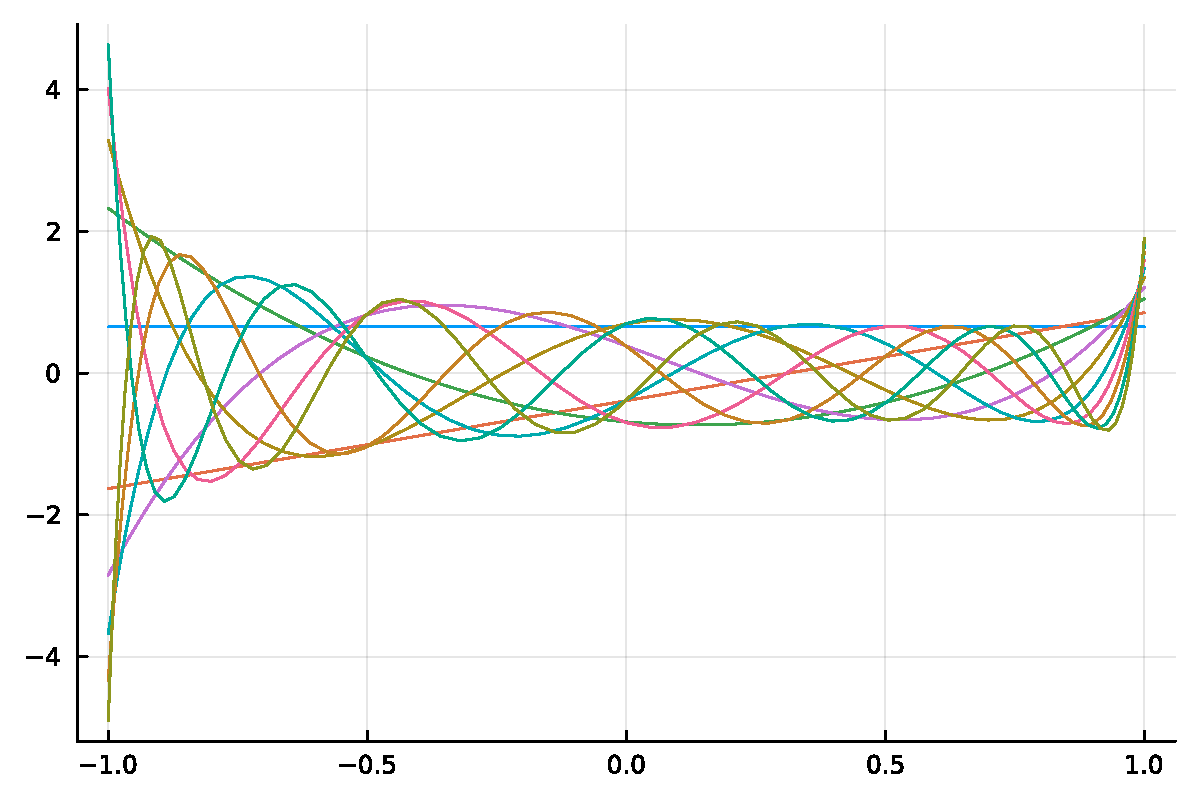
\includegraphics[width=\linewidth]{jl_dOthw0/OP_methods_7_1.pdf}

The three-term recurrence means we can simplify Gram\ensuremath{\endash}Schmidt, and calculate the recurrence coefficients at the same time:

\textbf{Proposition (Gram\ensuremath{\endash}Schmidt)} Define


\begin{align*}
p_0(x) &= 1 \\
q_0(x) &= {1 \over \| p_0\|}\\
a_n &= \langle x q_n, q_n \rangle \\
b_{n-1} &= \langle x q_n, q_{n-1}\rangle\\
p_{n+1}(x) &= x q_n(x) -  a_n q_n(x) -  b_{n-1} q_{n-1}(x)\\
q_{n+1}(x) &= {p_{n+1}(x) \over \|p_{n+1}\|}
\end{align*}
Then $q_0(x), q_1(x), \ldots$ are orthonormal w.r.t. $w$.

\textbf{Remark} This can be made a bit more efficient by using $\|p_{n+1}\|$ to calculate $b_n$.


\begin{lstlisting}
(*@\HLJLn{x}@*) (*@\HLJLoB{=}@*) (*@\HLJLnf{Fun}@*)(*@\HLJLp{()}@*)
(*@\HLJLn{w}@*) (*@\HLJLoB{=}@*) (*@\HLJLnf{exp}@*)(*@\HLJLp{(}@*)(*@\HLJLn{x}@*)(*@\HLJLp{)}@*)
(*@\HLJLn{ip}@*) (*@\HLJLoB{=}@*) (*@\HLJLp{(}@*)(*@\HLJLn{f}@*)(*@\HLJLp{,}@*)(*@\HLJLn{g}@*)(*@\HLJLp{)}@*) (*@\HLJLoB{->}@*) (*@\HLJLnf{sum}@*)(*@\HLJLp{(}@*)(*@\HLJLn{f}@*)(*@\HLJLoB{*}@*)(*@\HLJLn{g}@*)(*@\HLJLoB{*}@*)(*@\HLJLn{w}@*)(*@\HLJLp{)}@*)
(*@\HLJLn{nrm}@*) (*@\HLJLoB{=}@*) (*@\HLJLn{f}@*)    (*@\HLJLoB{->}@*) (*@\HLJLnf{sqrt}@*)(*@\HLJLp{(}@*)(*@\HLJLnf{ip}@*)(*@\HLJLp{(}@*)(*@\HLJLn{f}@*)(*@\HLJLp{,}@*)(*@\HLJLn{f}@*)(*@\HLJLp{))}@*)
(*@\HLJLn{n}@*) (*@\HLJLoB{=}@*) (*@\HLJLni{10}@*)
(*@\HLJLn{q}@*) (*@\HLJLoB{=}@*) (*@\HLJLnf{Array}@*)(*@\HLJLp{{\{}}@*)(*@\HLJLn{Fun}@*)(*@\HLJLp{{\}}(}@*)(*@\HLJLn{undef}@*)(*@\HLJLp{,}@*) (*@\HLJLn{n}@*)(*@\HLJLp{)}@*)
(*@\HLJLn{p}@*) (*@\HLJLoB{=}@*) (*@\HLJLnf{Array}@*)(*@\HLJLp{{\{}}@*)(*@\HLJLn{Fun}@*)(*@\HLJLp{{\}}(}@*)(*@\HLJLn{undef}@*)(*@\HLJLp{,}@*) (*@\HLJLn{n}@*)(*@\HLJLp{)}@*)
(*@\HLJLn{a}@*) (*@\HLJLoB{=}@*) (*@\HLJLnf{zeros}@*)(*@\HLJLp{(}@*)(*@\HLJLn{n}@*)(*@\HLJLp{)}@*)
(*@\HLJLn{b}@*) (*@\HLJLoB{=}@*) (*@\HLJLnf{zeros}@*)(*@\HLJLp{(}@*)(*@\HLJLn{n}@*)(*@\HLJLp{)}@*)
(*@\HLJLn{p}@*)(*@\HLJLp{[}@*)(*@\HLJLni{1}@*)(*@\HLJLp{]}@*) (*@\HLJLoB{=}@*) (*@\HLJLnf{Fun}@*)(*@\HLJLp{(}@*)(*@\HLJLni{1}@*)(*@\HLJLp{,}@*) (*@\HLJLoB{-}@*)(*@\HLJLni{1}@*) (*@\HLJLoB{..}@*) (*@\HLJLni{1}@*) (*@\HLJLp{)}@*)
(*@\HLJLn{q}@*)(*@\HLJLp{[}@*)(*@\HLJLni{1}@*)(*@\HLJLp{]}@*) (*@\HLJLoB{=}@*) (*@\HLJLn{p}@*)(*@\HLJLp{[}@*)(*@\HLJLni{1}@*)(*@\HLJLp{]}@*)(*@\HLJLoB{/}@*)(*@\HLJLnf{nrm}@*)(*@\HLJLp{(}@*)(*@\HLJLn{p}@*)(*@\HLJLp{[}@*)(*@\HLJLni{1}@*)(*@\HLJLp{])}@*)

(*@\HLJLn{p}@*)(*@\HLJLp{[}@*)(*@\HLJLni{2}@*)(*@\HLJLp{]}@*) (*@\HLJLoB{=}@*) (*@\HLJLn{x}@*)(*@\HLJLoB{*}@*)(*@\HLJLn{q}@*)(*@\HLJLp{[}@*)(*@\HLJLni{1}@*)(*@\HLJLp{]}@*)
(*@\HLJLn{a}@*)(*@\HLJLp{[}@*)(*@\HLJLni{1}@*)(*@\HLJLp{]}@*) (*@\HLJLoB{=}@*) (*@\HLJLnf{ip}@*)(*@\HLJLp{(}@*)(*@\HLJLn{p}@*)(*@\HLJLp{[}@*)(*@\HLJLni{2}@*)(*@\HLJLp{],}@*)(*@\HLJLn{q}@*)(*@\HLJLp{[}@*)(*@\HLJLni{1}@*)(*@\HLJLp{])}@*)
(*@\HLJLn{p}@*)(*@\HLJLp{[}@*)(*@\HLJLni{2}@*)(*@\HLJLp{]}@*) (*@\HLJLoB{-=}@*) (*@\HLJLn{a}@*)(*@\HLJLp{[}@*)(*@\HLJLni{1}@*)(*@\HLJLp{]}@*)(*@\HLJLoB{*}@*)(*@\HLJLn{q}@*)(*@\HLJLp{[}@*)(*@\HLJLni{1}@*)(*@\HLJLp{]}@*)
(*@\HLJLn{q}@*)(*@\HLJLp{[}@*)(*@\HLJLni{2}@*)(*@\HLJLp{]}@*) (*@\HLJLoB{=}@*) (*@\HLJLn{p}@*)(*@\HLJLp{[}@*)(*@\HLJLni{2}@*)(*@\HLJLp{]}@*)(*@\HLJLoB{/}@*)(*@\HLJLnf{nrm}@*)(*@\HLJLp{(}@*)(*@\HLJLn{p}@*)(*@\HLJLp{[}@*)(*@\HLJLni{2}@*)(*@\HLJLp{])}@*)

(*@\HLJLk{for}@*) (*@\HLJLn{k}@*)(*@\HLJLoB{=}@*)(*@\HLJLni{2}@*)(*@\HLJLoB{:}@*)(*@\HLJLn{n}@*)(*@\HLJLoB{-}@*)(*@\HLJLni{1}@*)
    (*@\HLJLn{p}@*)(*@\HLJLp{[}@*)(*@\HLJLn{k}@*)(*@\HLJLoB{+}@*)(*@\HLJLni{1}@*)(*@\HLJLp{]}@*) (*@\HLJLoB{=}@*) (*@\HLJLn{x}@*)(*@\HLJLoB{*}@*)(*@\HLJLn{q}@*)(*@\HLJLp{[}@*)(*@\HLJLn{k}@*)(*@\HLJLp{]}@*)
    (*@\HLJLn{b}@*)(*@\HLJLp{[}@*)(*@\HLJLn{k}@*)(*@\HLJLoB{-}@*)(*@\HLJLni{1}@*)(*@\HLJLp{]}@*) (*@\HLJLoB{=}@*)(*@\HLJLnf{ip}@*)(*@\HLJLp{(}@*)(*@\HLJLn{p}@*)(*@\HLJLp{[}@*)(*@\HLJLn{k}@*)(*@\HLJLoB{+}@*)(*@\HLJLni{1}@*)(*@\HLJLp{],}@*)(*@\HLJLn{q}@*)(*@\HLJLp{[}@*)(*@\HLJLn{k}@*)(*@\HLJLoB{-}@*)(*@\HLJLni{1}@*)(*@\HLJLp{])}@*)
    (*@\HLJLn{a}@*)(*@\HLJLp{[}@*)(*@\HLJLn{k}@*)(*@\HLJLp{]}@*) (*@\HLJLoB{=}@*) (*@\HLJLnf{ip}@*)(*@\HLJLp{(}@*)(*@\HLJLn{p}@*)(*@\HLJLp{[}@*)(*@\HLJLn{k}@*)(*@\HLJLoB{+}@*)(*@\HLJLni{1}@*)(*@\HLJLp{],}@*)(*@\HLJLn{q}@*)(*@\HLJLp{[}@*)(*@\HLJLn{k}@*)(*@\HLJLp{])}@*)
    (*@\HLJLn{p}@*)(*@\HLJLp{[}@*)(*@\HLJLn{k}@*)(*@\HLJLoB{+}@*)(*@\HLJLni{1}@*)(*@\HLJLp{]}@*) (*@\HLJLoB{=}@*) (*@\HLJLn{p}@*)(*@\HLJLp{[}@*)(*@\HLJLn{k}@*)(*@\HLJLoB{+}@*)(*@\HLJLni{1}@*)(*@\HLJLp{]}@*) (*@\HLJLoB{-}@*) (*@\HLJLn{a}@*)(*@\HLJLp{[}@*)(*@\HLJLn{k}@*)(*@\HLJLp{]}@*)(*@\HLJLn{q}@*)(*@\HLJLp{[}@*)(*@\HLJLn{k}@*)(*@\HLJLp{]}@*) (*@\HLJLoB{-}@*) (*@\HLJLn{b}@*)(*@\HLJLp{[}@*)(*@\HLJLn{k}@*)(*@\HLJLoB{-}@*)(*@\HLJLni{1}@*)(*@\HLJLp{]}@*)(*@\HLJLn{q}@*)(*@\HLJLp{[}@*)(*@\HLJLn{k}@*)(*@\HLJLoB{-}@*)(*@\HLJLni{1}@*)(*@\HLJLp{]}@*)
    (*@\HLJLn{q}@*)(*@\HLJLp{[}@*)(*@\HLJLn{k}@*)(*@\HLJLoB{+}@*)(*@\HLJLni{1}@*)(*@\HLJLp{]}@*) (*@\HLJLoB{=}@*) (*@\HLJLn{p}@*)(*@\HLJLp{[}@*)(*@\HLJLn{k}@*)(*@\HLJLoB{+}@*)(*@\HLJLni{1}@*)(*@\HLJLp{]}@*)(*@\HLJLoB{/}@*)(*@\HLJLnf{nrm}@*)(*@\HLJLp{(}@*)(*@\HLJLn{p}@*)(*@\HLJLp{[}@*)(*@\HLJLn{k}@*)(*@\HLJLoB{+}@*)(*@\HLJLni{1}@*)(*@\HLJLp{])}@*)
(*@\HLJLk{end}@*)

(*@\HLJLnf{ip}@*)(*@\HLJLp{(}@*)(*@\HLJLn{q}@*)(*@\HLJLp{[}@*)(*@\HLJLni{5}@*)(*@\HLJLp{],}@*)(*@\HLJLn{q}@*)(*@\HLJLp{[}@*)(*@\HLJLni{2}@*)(*@\HLJLp{])}@*) (*@\HLJLcs{{\#}}@*) (*@\HLJLcs{shows}@*) (*@\HLJLcs{orthogonality}@*) (*@\HLJLcs{(to}@*) (*@\HLJLcs{numerical}@*) (*@\HLJLcs{accuracy)}@*)
\end{lstlisting}

\begin{lstlisting}
8.118505867571457e-16
\end{lstlisting}


Here we see a plot of the first 10 polynomials:


\begin{lstlisting}
(*@\HLJLn{p}@*) (*@\HLJLoB{=}@*) (*@\HLJLnf{plot}@*)(*@\HLJLp{(;}@*) (*@\HLJLn{legend}@*)(*@\HLJLoB{=}@*)(*@\HLJLkc{false}@*)(*@\HLJLp{)}@*)
(*@\HLJLk{for}@*) (*@\HLJLn{k}@*)(*@\HLJLoB{=}@*)(*@\HLJLni{1}@*)(*@\HLJLoB{:}@*)(*@\HLJLni{10}@*)
    (*@\HLJLnf{plot!}@*)(*@\HLJLp{(}@*)(*@\HLJLn{q}@*)(*@\HLJLp{[}@*)(*@\HLJLn{k}@*)(*@\HLJLp{])}@*)
(*@\HLJLk{end}@*)
(*@\HLJLn{p}@*)
\end{lstlisting}

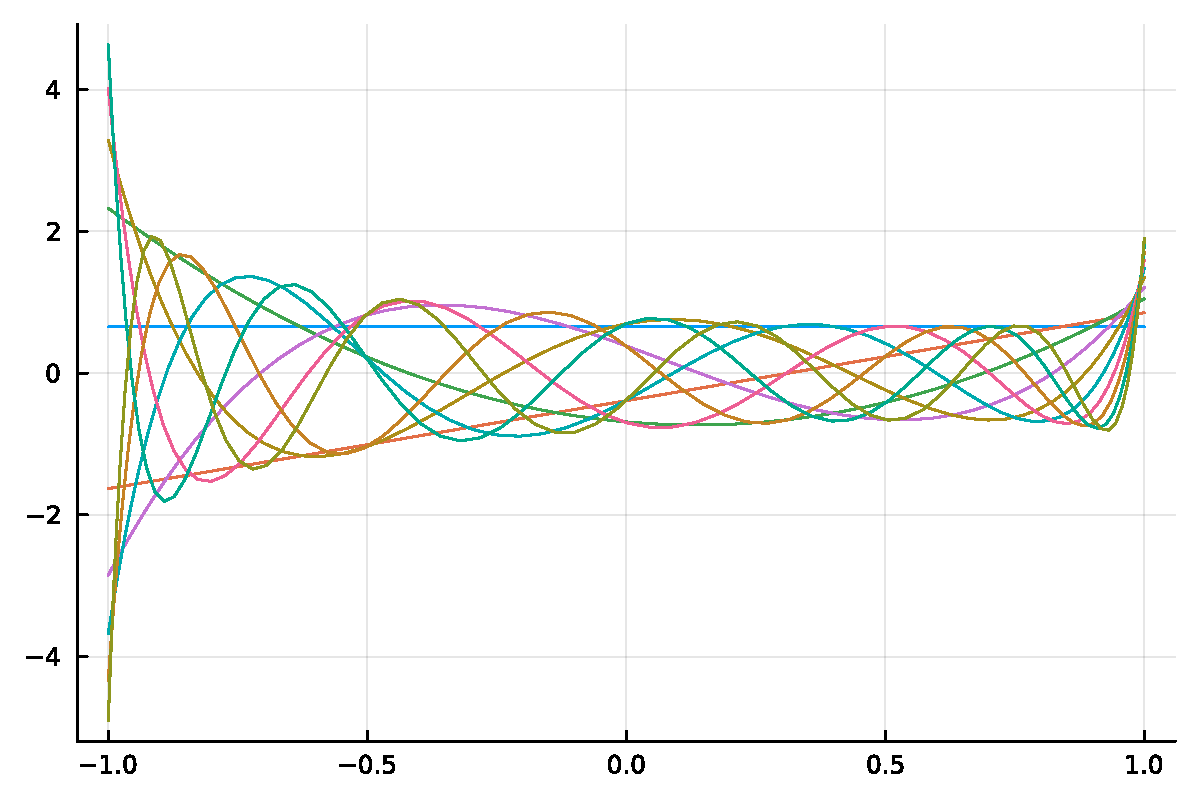
\includegraphics[width=\linewidth]{jl_dOthw0/OP_methods_9_1.pdf}

\subsection{2. Classical orthogonal polynomials}
Classical orthogonal polynomials are special families of orthogonal polynomials with a number of beautiful properties, for example

\begin{itemize}
\item[1. ] Their derivatives are also OPs


\item[2. ] They are eigenfunctions of simple differential operators

\end{itemize}
As stated above orthogonal polynomials are uniquely defined by the weight $w(x)$ and the constant $k_n$. We consider:

\begin{itemize}
\item[1. ] Chebyshev polynomials (1st kind) $T_n(x)$: $w(x) = 1/\sqrt{1-x^2}$ on $[-1,1]$.


\item[2. ] Chebyshev polynomials (2nd kind) $U_n(x)$: $\sqrt{1-x^2}$ on $[-1,1]$.


\item[3. ] Legendre polynomials $P_n(x)$: $w(x) = 1$ on $[-1,1]$.


\item[4. ] Ultrapsherical polynomials (my fav!): $C_n^{(\ensuremath{\lambda})}(x)$: $w(x) = (1-x^2)^{\ensuremath{\lambda}-1/2}$ on $[-1,1]$, $\ensuremath{\lambda} \ensuremath{\ne} 0$, $\ensuremath{\lambda} > -1/2$.


\item[5. ] Jacobi polynomials: $P_n^{(a,b)}(x)$: $w(x) = (1-x)^a (1+x)^b$ on $[-1,1]$, $a,b > -1$.


\item[6. ] Laguerre polynomials: $L_n(x)$: $w(x) = \exp(-x)$ on $[0,\ensuremath{\infty})$.


\item[7. ] Hermite polynomials $H_n(x)$: $w(x) = \exp(-x^2)$  on $(-\ensuremath{\infty},\ensuremath{\infty})$.

\end{itemize}
In the notes we will discuss properties of $T_n(x)$ and $P_n(x)$.

\subsubsection{Chebyshev}
\textbf{Definition (Chebyshev polynomials, 1st kind)} $T_n(x)$ are orthogonal with respect to $1/\sqrt{1-x^2}$ and satisfy:


\begin{align*}
T_0(x) &= 1, \\
T_n(x) &= 2^{n-1} x^n + O(x^{n-1})
\end{align*}
\textbf{Definition (Chebyshev polynomials, 2nd kind)} $U_n(x)$ are orthogonal with respect to $\sqrt{1-x^2}$.

\[
U_n(x) = 2^n x^n + O(x^{n-1})
\]
\textbf{Theorem (Chebyshev T are cos)}

\[
T_n(x) = \cos n\, {\rm acos}\, x
\]
In other words

\[
T_n(\cos(\ensuremath{\theta})) = \cos n \ensuremath{\theta}.
\]
\textbf{Proof}

We need to show that $p_n(x) := \cos n\, {\rm acos}\, x$ are

\begin{itemize}
\item[1. ] graded polynomials


\item[2. ] orthogonal w.r.t. $1/\sqrt{1-x^2}$ on $[-1,1]$, and


\item[3. ] have the right normalisation constant $k_n = 2^{n-1}$ for $n = 1,\ensuremath{\ldots}$.

\end{itemize}
Property (2) follows under a change of variables:

\[
\langle p_n, p_m \rangle = \int_{-1}^1 {p_n(x) p_m(x) \over \sqrt{1-x^2}} {\rm d} x =
\int_{-\ensuremath{\pi}}^\ensuremath{\pi} {\cos(n\ensuremath{\theta}) \cos(m\ensuremath{\theta}) \over \sqrt{1-\cos^2 \ensuremath{\theta}}} \sin \ensuremath{\theta} {\rm d} \ensuremath{\theta} =
\int_{-\ensuremath{\pi}}^\ensuremath{\pi} \cos(n\ensuremath{\theta}) \cos(m\ensuremath{\theta}) {\rm d} x = 0
\]
if $n \ensuremath{\ne} m$.

To see that they are graded we use the fact that

\[
x p_n(x) = \cos \ensuremath{\theta} \cos n \ensuremath{\theta} = {\cos(n-1)\ensuremath{\theta} + \cos(n+1)\ensuremath{\theta} \over 2} = {p_{n-1}(x) + p_{n+1}(x) \over 2}
\]
In other words $p_{n+1}(x) = 2x p_n(x) - p_{n-1}(x)$ for $n \geq 1$. Since each time we multiply by $2x$ and $p_0(x) = 1$, $p_1(x)=x$ we have

\[
p_{n+1}(x) = (2x)^n + O(x^{n-1})
\]
which completes the proof.

\[
\blacksquare
\]
Buried in the proof is the 3-term recurrence:

\textbf{Corollary}


\begin{align*}
x T_0(x) = T_1(x) \\
x T_n(x) = {T_{n-1}(x) + T_{n+1}(x) \over 2}
\end{align*}
Chebyshev polynomials are particularly powerful as their expansions are cosine series in disguise: for

\[
f(x) = \ensuremath{\sum}_{k=0}^\ensuremath{\infty} \check{f}_k T_k(x)
\]
we have

\[
f(\cos \ensuremath{\theta}) = \ensuremath{\sum}_{k=0}^\ensuremath{\infty} \check{f}_k \cos k \ensuremath{\theta}.
\]
Thus the coefficients can be recovered fast using FFT-based techniques as discussed in the problem sheet.

In the problem sheet we will also show the following:

\textbf{Theorem (Chebyshev U are sin)} For $x = \cos \ensuremath{\theta}$,

\[
U_n(x) = {\sin(n+1) \ensuremath{\theta} \over \sin \ensuremath{\theta}}
\]
which satisfy:


\begin{align*}
x U_0(x) &= U_1(x)/2 \\
x U_n(x) &= {U_{n-1}(x) \over 2} + {U_{n+1}(x) \over 2}.
\end{align*}
\subsubsection{Legendre}
\textbf{Definition (Legendre)} Legendre polynomials $P_n(x)$ are orthogonal polynomials with respect to $w(x) = 1$ on $[-1,1]$, with

\[
k_n = {1 \over 2^n} \begin{pmatrix} 2n \\ n \end{pmatrix} = 
{(2n)! \over 2^n (n!)^2}
\]
The reason for this complicated normalisation constant is both historical and that it leads to simpler formulae for recurrence relationships.

Classical orthogonal polynomials have \emph{Rodriguez formulae}, defining orthogonal polynomials as high order derivatives of simple functions. In this case we have:

\textbf{Lemma (Legendre Rodriguez formula)}

\[
P_n(x) = {1 \over (-2)^n n!}{{\rm d}^n \over {\rm d} x^n} (1-x^2)^n
\]
\textbf{Proof} We need to verify:

\begin{itemize}
\item[1. ] graded polynomials


\item[2. ] orthogonal to all lower degree polynomials on $[-1,1]$, and


\item[3. ] have the right normalisation constant $k_n = {1 \over 2^n} \begin{pmatrix} 2n \\ n \end{pmatrix}$.

\end{itemize}
(1) follows since its a degree $n$ polynomial (the $n$-th derivative of a degree $2n$ polynomial). (2) follows by integration by parts. Note that $(1-x^2)^n$ and its first $n-1$ derivatives vanish at $\ensuremath{\pm}1$. If $r_m$ is a degree $m < n$ polynomial we have:

\[
\ensuremath{\int}_{-1}^1 {{\rm d}^n \over {\rm d} x^n} (1-x^2)^n r_m(x) {\rm d}x
= -\ensuremath{\int}_{-1}^1 {{\rm d}^{n-1} \over {\rm d} x^{n-1}} (1-x^2)^n r_m'(x) {\rm d}x =
\ensuremath{\cdots} = (-)^n \ensuremath{\int}_{-1}^1 (1-x^2) r_m^{(n)}(x) {\rm d}x = 0.
\]
(3) follows since:


\begin{align*}
{{\rm d}^n \over {\rm d} x^n}[(-)^n x^{2n} + O(x^{2n-1})] &=
(-)^n 2n {{\rm d}^{n-1} \over {\rm d} x^{n-1}} x^{2n-1}+ O(x^{2n-1})] \\
&=
(-)^n 2n (2n-1) {{\rm d}^{n-2} \over {\rm d} x^{n-2}} x^{2n-2}+ O(x^{2n-2})] = \ensuremath{\cdots} \\
&= (-)^n 2n (2n-1) \ensuremath{\cdots} (n+1) x^n + O(x^{n-1}) = 
(-)^n {(2n)! \over n!} x^n + O(x^{n-1})
\end{align*}
\[
\blacksquare
\]
This allows us to determine the coefficients $k_n^{(\ensuremath{\lambda})}$ which are useful in proofs. In particular we will use $k_n^{(1)}$:

\textbf{Lemma (Legendre monomial coefficients)}


\begin{align*}
P_0(x) &= 1 \\
P_1(x) &= x \\
P_n(x) &= \underbrace{{(2n)! \over 2^n (n!)^2}}_{k_n} x^n - \underbrace{(2n-2)! \over 2^n (n-2)! (n-1)!}_{k_n^{(2)}} x^{n-2} + O(x^{n-4})
\end{align*}
(Here the $O(x^{n-4})$ is as $x \ensuremath{\rightarrow} \ensuremath{\infty}$, which implies that the term is a polynomial of degree $\ensuremath{\leq} n-4$. For $n = 2,3$ the $O(x^{n-4})$ term is therefore precisely zero.)

\textbf{Proof}

The $n=0$ and $1$ case are immediate. For the other case we expand $(1-x^2)^n$ to get:


\begin{align*}
(-)^n {{\rm d}^n \over {\rm d} x^n} (1-x^2)^n &=
{{\rm d}^n \over {\rm d} x^n} [ x^{2n} - n x^{2n-2} + O(x^{2n-4})]\\
&= (2n)\ensuremath{\cdots}(2n-n+1) x^n - n (2n-2)\ensuremath{\cdots}(2n-2-n+1) x^{n-2} + O(x^{n-4}) \\
&= {(2n)! \over n!} x^n - {n (2n-2)! \over (n-2)!} x^{n-2} + O(x^{n-4})
\end{align*}
Multiplying through by ${1 \over 2^n (n!)}$ completes the derivation.

\[
\blacksquare
\]
\textbf{Theorem (Legendre 3-term recurrence)}


\begin{align*}
xP_0(x) &= P_1(x) \\
(2n+1) xP_n(x) &= nP_{n-1}(x) + (n+1)P_{n+1}(x)
\end{align*}
\textbf{Proof}  The $n = 0$ case is immediate (since $w(x) = w(-x)$ $a_n = 0$, from PS8). For the other cases we match terms:

\[
(2n+1)xP_n(x) - n P_{n-1}(x) - (n+1)P_{n+1}(x) = [(2n+1)k_n - (n+1) k_{n+1}] x^{n+1} + [(2n+1) k_n^{(1)} -n k_{n-1} - (n+1) k_{n+1}^{(1)}] x^{n-1} + O(x^{n-3})
\]
Using the expressions for $k_n$ and $k_n^{(1)}$ above we have (leaving the manipulations as an exercise):


\begin{align*}
(2n+1)k_n - (n+1) k_{n+1} = {(2n+1)! \over 2^n (n!)^2} - (n+1) {(2n+2)! \over 2^(n+1) ((n+1)!)^2} = 0 \\
(2n+1) k_n^{(1)} -n k_{n-1}  - (n+1) k_{n+1}^{(1)} =  -(2n+1) {(2n-2)! \over 2^n (n-2)! (n-1)!} - n {(2n-2)! \over 2^{n-1} ((n-1)!)^2} + (n+1){(2n)! \over 2^{n+1} (n-1)! n!} = 0
\end{align*}
Thus

\[
(2n+1)xP_n(x) - n P_{n-1}(x) - (n+1)P_{n+1}(x) = O(x^{n-3})
\]
But as it is orthogonal to $P_k(x)$ for $0 \ensuremath{\leq} k \ensuremath{\leq} n-3$ it must be zero. $\blacksquare$

We will also investigate the properties of \emph{classical} OPs. A good reference is  \href{http://dlmf.nist.gov/18}{Digital Library of Mathematical Functions, Chapter 18}.

This lecture we discuss

\begin{itemize}
\item[1. ] Hermite, Laguerre, and Jacobi polynomials


\item[2. ] Legendre, Chebyshev, and ultraspherical polynomials


\item[3. ] Explicit construction for Chebyshev polynomials

\end{itemize}
\subsection{Definition of classical orthogonal polynomials}
Classical orthogonal polynomials are orthogonal with respect to the following three weights:

\begin{tabular}
{l | l | l | l | l}
Name & $(a,b)$ & $w(x)$ & Notation & $k_n$ \\
\hline
Hermite & $(-\infty,\infty)$ & ${\rm e}^{-x^2}$ & $H_n(x)$ & $2^n$ \\
Laguerre & $(0,\infty)$ & $x^\alpha {\rm e}^{-x}$ & $L_n^{(\alpha)}(x)$ & \href{http://dlmf.nist.gov/18.3}{Table 18.3.1} \\
Jacobi & $(-1,1)$ & $(1-x)^{\alpha} (1+x)^\beta$ & $P_n^{(\alpha,\beta)}(x)$ & \href{http://dlmf.nist.gov/18.3}{Table 18.3.1} \\
\end{tabular}
Note out of convention the parameters for Jacobi polynomials are right-to-left order.

We can actually construct these polynomials in Julia, first consider Hermite:


\begin{lstlisting}
(*@\HLJLk{using}@*) (*@\HLJLn{ApproxFun}@*)(*@\HLJLp{,}@*) (*@\HLJLn{Plots}@*)(*@\HLJLp{,}@*) (*@\HLJLn{LinearAlgebra}@*)(*@\HLJLp{,}@*) (*@\HLJLn{ComplexPhasePortrait}@*)
(*@\HLJLn{H\ensuremath{\_0}}@*) (*@\HLJLoB{=}@*) (*@\HLJLnf{Fun}@*)(*@\HLJLp{(}@*)(*@\HLJLnf{Hermite}@*)(*@\HLJLp{(),}@*) (*@\HLJLp{[}@*)(*@\HLJLni{1}@*)(*@\HLJLp{])}@*)
(*@\HLJLn{H\ensuremath{\_1}}@*) (*@\HLJLoB{=}@*) (*@\HLJLnf{Fun}@*)(*@\HLJLp{(}@*)(*@\HLJLnf{Hermite}@*)(*@\HLJLp{(),}@*) (*@\HLJLp{[}@*)(*@\HLJLni{0}@*)(*@\HLJLp{,}@*)(*@\HLJLni{1}@*)(*@\HLJLp{])}@*)
(*@\HLJLn{H\ensuremath{\_2}}@*) (*@\HLJLoB{=}@*) (*@\HLJLnf{Fun}@*)(*@\HLJLp{(}@*)(*@\HLJLnf{Hermite}@*)(*@\HLJLp{(),}@*) (*@\HLJLp{[}@*)(*@\HLJLni{0}@*)(*@\HLJLp{,}@*)(*@\HLJLni{0}@*)(*@\HLJLp{,}@*)(*@\HLJLni{1}@*)(*@\HLJLp{])}@*)
(*@\HLJLn{H\ensuremath{\_3}}@*) (*@\HLJLoB{=}@*) (*@\HLJLnf{Fun}@*)(*@\HLJLp{(}@*)(*@\HLJLnf{Hermite}@*)(*@\HLJLp{(),}@*) (*@\HLJLp{[}@*)(*@\HLJLni{0}@*)(*@\HLJLp{,}@*)(*@\HLJLni{0}@*)(*@\HLJLp{,}@*)(*@\HLJLni{0}@*)(*@\HLJLp{,}@*)(*@\HLJLni{1}@*)(*@\HLJLp{])}@*)
(*@\HLJLn{H\ensuremath{\_4}}@*) (*@\HLJLoB{=}@*) (*@\HLJLnf{Fun}@*)(*@\HLJLp{(}@*)(*@\HLJLnf{Hermite}@*)(*@\HLJLp{(),}@*) (*@\HLJLp{[}@*)(*@\HLJLni{0}@*)(*@\HLJLp{,}@*)(*@\HLJLni{0}@*)(*@\HLJLp{,}@*)(*@\HLJLni{0}@*)(*@\HLJLp{,}@*)(*@\HLJLni{0}@*)(*@\HLJLp{,}@*)(*@\HLJLni{1}@*)(*@\HLJLp{])}@*)
(*@\HLJLn{H\ensuremath{\_5}}@*) (*@\HLJLoB{=}@*) (*@\HLJLnf{Fun}@*)(*@\HLJLp{(}@*)(*@\HLJLnf{Hermite}@*)(*@\HLJLp{(),}@*) (*@\HLJLp{[}@*)(*@\HLJLni{0}@*)(*@\HLJLp{,}@*)(*@\HLJLni{0}@*)(*@\HLJLp{,}@*)(*@\HLJLni{0}@*)(*@\HLJLp{,}@*)(*@\HLJLni{0}@*)(*@\HLJLp{,}@*)(*@\HLJLni{0}@*)(*@\HLJLp{,}@*)(*@\HLJLni{1}@*)(*@\HLJLp{])}@*)

(*@\HLJLn{xx}@*) (*@\HLJLoB{=}@*) (*@\HLJLoB{-}@*)(*@\HLJLni{4}@*)(*@\HLJLoB{:}@*)(*@\HLJLnfB{0.01}@*)(*@\HLJLoB{:}@*)(*@\HLJLni{4}@*)
(*@\HLJLnf{plot}@*)(*@\HLJLp{(}@*)(*@\HLJLn{xx}@*)(*@\HLJLp{,}@*) (*@\HLJLn{H\ensuremath{\_0}}@*)(*@\HLJLoB{.}@*)(*@\HLJLp{(}@*)(*@\HLJLn{xx}@*)(*@\HLJLp{);}@*) (*@\HLJLn{label}@*)(*@\HLJLoB{=}@*)(*@\HLJLs{"{}H{\_}0"{}}@*)(*@\HLJLp{,}@*) (*@\HLJLn{ylims}@*)(*@\HLJLoB{=}@*)(*@\HLJLp{(}@*)(*@\HLJLoB{-}@*)(*@\HLJLni{400}@*)(*@\HLJLp{,}@*)(*@\HLJLni{400}@*)(*@\HLJLp{))}@*)
(*@\HLJLnf{plot!}@*)(*@\HLJLp{(}@*)(*@\HLJLn{xx}@*)(*@\HLJLp{,}@*) (*@\HLJLn{H\ensuremath{\_1}}@*)(*@\HLJLoB{.}@*)(*@\HLJLp{(}@*)(*@\HLJLn{xx}@*)(*@\HLJLp{);}@*) (*@\HLJLn{label}@*)(*@\HLJLoB{=}@*)(*@\HLJLs{"{}H{\_}1"{}}@*)(*@\HLJLp{,}@*) (*@\HLJLn{ylims}@*)(*@\HLJLoB{=}@*)(*@\HLJLp{(}@*)(*@\HLJLoB{-}@*)(*@\HLJLni{400}@*)(*@\HLJLp{,}@*)(*@\HLJLni{400}@*)(*@\HLJLp{))}@*)
(*@\HLJLnf{plot!}@*)(*@\HLJLp{(}@*)(*@\HLJLn{xx}@*)(*@\HLJLp{,}@*) (*@\HLJLn{H\ensuremath{\_2}}@*)(*@\HLJLoB{.}@*)(*@\HLJLp{(}@*)(*@\HLJLn{xx}@*)(*@\HLJLp{);}@*) (*@\HLJLn{label}@*)(*@\HLJLoB{=}@*)(*@\HLJLs{"{}H{\_}2"{}}@*)(*@\HLJLp{,}@*) (*@\HLJLn{ylims}@*)(*@\HLJLoB{=}@*)(*@\HLJLp{(}@*)(*@\HLJLoB{-}@*)(*@\HLJLni{400}@*)(*@\HLJLp{,}@*)(*@\HLJLni{400}@*)(*@\HLJLp{))}@*)
(*@\HLJLnf{plot!}@*)(*@\HLJLp{(}@*)(*@\HLJLn{xx}@*)(*@\HLJLp{,}@*) (*@\HLJLn{H\ensuremath{\_3}}@*)(*@\HLJLoB{.}@*)(*@\HLJLp{(}@*)(*@\HLJLn{xx}@*)(*@\HLJLp{);}@*) (*@\HLJLn{label}@*)(*@\HLJLoB{=}@*)(*@\HLJLs{"{}H{\_}3"{}}@*)(*@\HLJLp{,}@*) (*@\HLJLn{ylims}@*)(*@\HLJLoB{=}@*)(*@\HLJLp{(}@*)(*@\HLJLoB{-}@*)(*@\HLJLni{400}@*)(*@\HLJLp{,}@*)(*@\HLJLni{400}@*)(*@\HLJLp{))}@*)
(*@\HLJLnf{plot!}@*)(*@\HLJLp{(}@*)(*@\HLJLn{xx}@*)(*@\HLJLp{,}@*) (*@\HLJLn{H\ensuremath{\_4}}@*)(*@\HLJLoB{.}@*)(*@\HLJLp{(}@*)(*@\HLJLn{xx}@*)(*@\HLJLp{);}@*) (*@\HLJLn{label}@*)(*@\HLJLoB{=}@*)(*@\HLJLs{"{}H{\_}4"{}}@*)(*@\HLJLp{,}@*) (*@\HLJLn{ylims}@*)(*@\HLJLoB{=}@*)(*@\HLJLp{(}@*)(*@\HLJLoB{-}@*)(*@\HLJLni{400}@*)(*@\HLJLp{,}@*)(*@\HLJLni{400}@*)(*@\HLJLp{))}@*)
(*@\HLJLnf{plot!}@*)(*@\HLJLp{(}@*)(*@\HLJLn{xx}@*)(*@\HLJLp{,}@*) (*@\HLJLn{H\ensuremath{\_5}}@*)(*@\HLJLoB{.}@*)(*@\HLJLp{(}@*)(*@\HLJLn{xx}@*)(*@\HLJLp{);}@*) (*@\HLJLn{label}@*)(*@\HLJLoB{=}@*)(*@\HLJLs{"{}H{\_}5"{}}@*)(*@\HLJLp{)}@*)
\end{lstlisting}

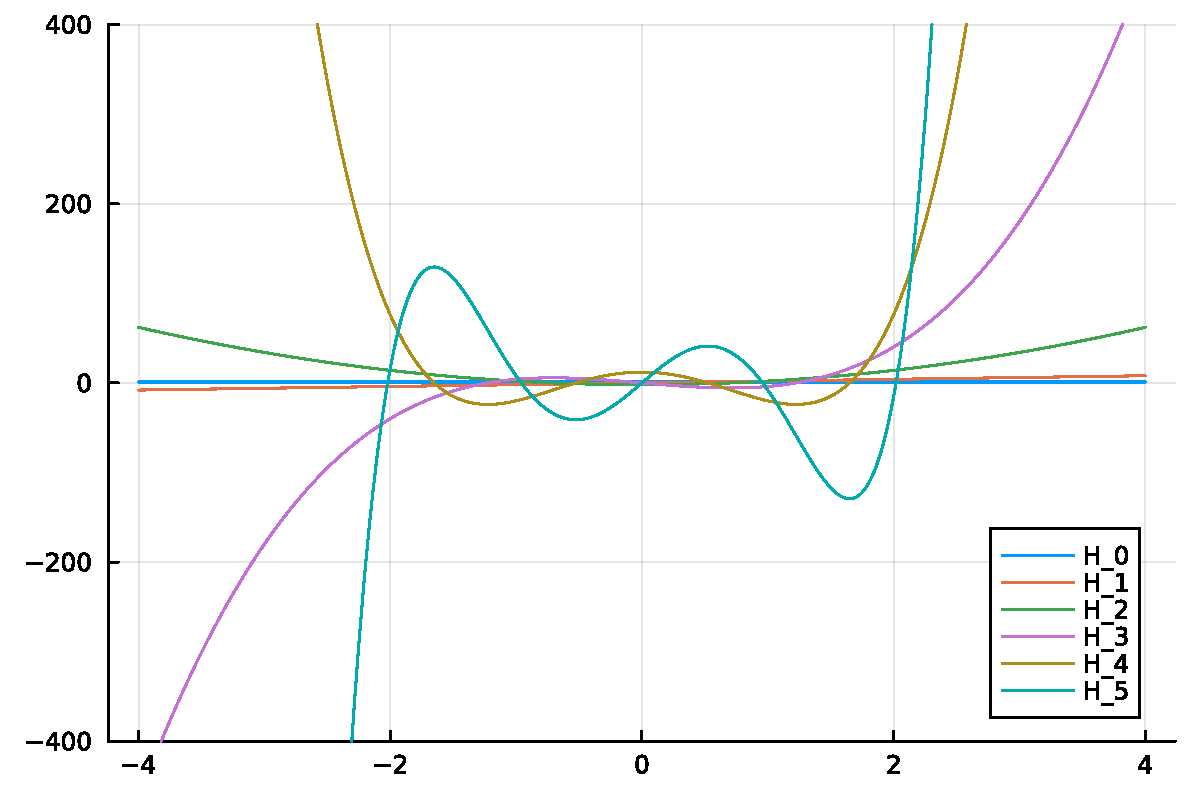
\includegraphics[width=\linewidth]{jl_dOthw0/OP_methods_10_1.pdf}

We verify their orthogonality:


\begin{lstlisting}
(*@\HLJLn{w}@*) (*@\HLJLoB{=}@*) (*@\HLJLnf{Fun}@*)(*@\HLJLp{(}@*)(*@\HLJLnf{GaussWeight}@*)(*@\HLJLp{(),}@*) (*@\HLJLp{[}@*)(*@\HLJLnfB{1.0}@*)(*@\HLJLp{])}@*)

(*@\HLJLnd{@show}@*) (*@\HLJLnf{sum}@*)(*@\HLJLp{(}@*)(*@\HLJLn{H\ensuremath{\_2}}@*)(*@\HLJLoB{*}@*)(*@\HLJLn{H\ensuremath{\_5}}@*)(*@\HLJLoB{*}@*)(*@\HLJLn{w}@*)(*@\HLJLp{)}@*)  (*@\HLJLcs{{\#}}@*) (*@\HLJLcs{means}@*) (*@\HLJLcs{integrate}@*)
(*@\HLJLnd{@show}@*) (*@\HLJLnf{sum}@*)(*@\HLJLp{(}@*)(*@\HLJLn{H\ensuremath{\_5}}@*)(*@\HLJLoB{*}@*)(*@\HLJLn{H\ensuremath{\_5}}@*)(*@\HLJLoB{*}@*)(*@\HLJLn{w}@*)(*@\HLJLp{);}@*)
\end{lstlisting}

\begin{lstlisting}
sum(H(*@\ensuremath{\_2}@*) * H(*@\ensuremath{\_5}@*) * w) = 0.0
sum(H(*@\ensuremath{\_5}@*) * H(*@\ensuremath{\_5}@*) * w) = 6806.222787477181
\end{lstlisting}


Now Jacobi:


\begin{lstlisting}
(*@\HLJLn{\ensuremath{\alpha}}@*)(*@\HLJLp{,}@*)(*@\HLJLn{\ensuremath{\beta}}@*) (*@\HLJLoB{=}@*) (*@\HLJLnfB{0.1}@*)(*@\HLJLp{,}@*)(*@\HLJLnfB{0.2}@*)
(*@\HLJLn{P\ensuremath{\_0}}@*) (*@\HLJLoB{=}@*) (*@\HLJLnf{Fun}@*)(*@\HLJLp{(}@*)(*@\HLJLnf{Jacobi}@*)(*@\HLJLp{(}@*)(*@\HLJLn{\ensuremath{\beta}}@*)(*@\HLJLp{,}@*)(*@\HLJLn{\ensuremath{\alpha}}@*)(*@\HLJLp{),}@*) (*@\HLJLp{[}@*)(*@\HLJLni{1}@*)(*@\HLJLp{])}@*)
(*@\HLJLn{P\ensuremath{\_1}}@*) (*@\HLJLoB{=}@*) (*@\HLJLnf{Fun}@*)(*@\HLJLp{(}@*)(*@\HLJLnf{Jacobi}@*)(*@\HLJLp{(}@*)(*@\HLJLn{\ensuremath{\beta}}@*)(*@\HLJLp{,}@*)(*@\HLJLn{\ensuremath{\alpha}}@*)(*@\HLJLp{),}@*) (*@\HLJLp{[}@*)(*@\HLJLni{0}@*)(*@\HLJLp{,}@*)(*@\HLJLni{1}@*)(*@\HLJLp{])}@*)
(*@\HLJLn{P\ensuremath{\_2}}@*) (*@\HLJLoB{=}@*) (*@\HLJLnf{Fun}@*)(*@\HLJLp{(}@*)(*@\HLJLnf{Jacobi}@*)(*@\HLJLp{(}@*)(*@\HLJLn{\ensuremath{\beta}}@*)(*@\HLJLp{,}@*)(*@\HLJLn{\ensuremath{\alpha}}@*)(*@\HLJLp{),}@*) (*@\HLJLp{[}@*)(*@\HLJLni{0}@*)(*@\HLJLp{,}@*)(*@\HLJLni{0}@*)(*@\HLJLp{,}@*)(*@\HLJLni{1}@*)(*@\HLJLp{])}@*)
(*@\HLJLn{P\ensuremath{\_3}}@*) (*@\HLJLoB{=}@*) (*@\HLJLnf{Fun}@*)(*@\HLJLp{(}@*)(*@\HLJLnf{Jacobi}@*)(*@\HLJLp{(}@*)(*@\HLJLn{\ensuremath{\beta}}@*)(*@\HLJLp{,}@*)(*@\HLJLn{\ensuremath{\alpha}}@*)(*@\HLJLp{),}@*) (*@\HLJLp{[}@*)(*@\HLJLni{0}@*)(*@\HLJLp{,}@*)(*@\HLJLni{0}@*)(*@\HLJLp{,}@*)(*@\HLJLni{0}@*)(*@\HLJLp{,}@*)(*@\HLJLni{1}@*)(*@\HLJLp{])}@*)
(*@\HLJLn{P\ensuremath{\_4}}@*) (*@\HLJLoB{=}@*) (*@\HLJLnf{Fun}@*)(*@\HLJLp{(}@*)(*@\HLJLnf{Jacobi}@*)(*@\HLJLp{(}@*)(*@\HLJLn{\ensuremath{\beta}}@*)(*@\HLJLp{,}@*)(*@\HLJLn{\ensuremath{\alpha}}@*)(*@\HLJLp{),}@*) (*@\HLJLp{[}@*)(*@\HLJLni{0}@*)(*@\HLJLp{,}@*)(*@\HLJLni{0}@*)(*@\HLJLp{,}@*)(*@\HLJLni{0}@*)(*@\HLJLp{,}@*)(*@\HLJLni{0}@*)(*@\HLJLp{,}@*)(*@\HLJLni{1}@*)(*@\HLJLp{])}@*)
(*@\HLJLn{P\ensuremath{\_5}}@*) (*@\HLJLoB{=}@*) (*@\HLJLnf{Fun}@*)(*@\HLJLp{(}@*)(*@\HLJLnf{Jacobi}@*)(*@\HLJLp{(}@*)(*@\HLJLn{\ensuremath{\beta}}@*)(*@\HLJLp{,}@*)(*@\HLJLn{\ensuremath{\alpha}}@*)(*@\HLJLp{),}@*) (*@\HLJLp{[}@*)(*@\HLJLni{0}@*)(*@\HLJLp{,}@*)(*@\HLJLni{0}@*)(*@\HLJLp{,}@*)(*@\HLJLni{0}@*)(*@\HLJLp{,}@*)(*@\HLJLni{0}@*)(*@\HLJLp{,}@*)(*@\HLJLni{0}@*)(*@\HLJLp{,}@*)(*@\HLJLni{1}@*)(*@\HLJLp{])}@*)

(*@\HLJLn{xx}@*) (*@\HLJLoB{=}@*) (*@\HLJLoB{-}@*)(*@\HLJLni{1}@*)(*@\HLJLoB{:}@*)(*@\HLJLnfB{0.01}@*)(*@\HLJLoB{:}@*)(*@\HLJLni{1}@*)
(*@\HLJLnf{plot}@*)(*@\HLJLp{(}@*) (*@\HLJLn{xx}@*)(*@\HLJLp{,}@*) (*@\HLJLn{P\ensuremath{\_0}}@*)(*@\HLJLoB{.}@*)(*@\HLJLp{(}@*)(*@\HLJLn{xx}@*)(*@\HLJLp{);}@*) (*@\HLJLn{label}@*)(*@\HLJLoB{=}@*)(*@\HLJLs{"{}P{\_}0{\textasciicircum}(}@*)(*@\HLJLsi{{\$}\ensuremath{\alpha}}@*)(*@\HLJLs{,}@*)(*@\HLJLsi{{\$}\ensuremath{\beta}}@*)(*@\HLJLs{)"{}}@*)(*@\HLJLp{,}@*) (*@\HLJLn{ylims}@*)(*@\HLJLoB{=}@*)(*@\HLJLp{(}@*)(*@\HLJLoB{-}@*)(*@\HLJLni{2}@*)(*@\HLJLp{,}@*)(*@\HLJLni{2}@*)(*@\HLJLp{))}@*)
(*@\HLJLnf{plot!}@*)(*@\HLJLp{(}@*)(*@\HLJLn{xx}@*)(*@\HLJLp{,}@*) (*@\HLJLn{P\ensuremath{\_1}}@*)(*@\HLJLoB{.}@*)(*@\HLJLp{(}@*)(*@\HLJLn{xx}@*)(*@\HLJLp{);}@*) (*@\HLJLn{label}@*)(*@\HLJLoB{=}@*)(*@\HLJLs{"{}P{\_}1{\textasciicircum}(}@*)(*@\HLJLsi{{\$}\ensuremath{\alpha}}@*)(*@\HLJLs{,}@*)(*@\HLJLsi{{\$}\ensuremath{\beta}}@*)(*@\HLJLs{)"{}}@*)(*@\HLJLp{)}@*)
(*@\HLJLnf{plot!}@*)(*@\HLJLp{(}@*)(*@\HLJLn{xx}@*)(*@\HLJLp{,}@*) (*@\HLJLn{P\ensuremath{\_2}}@*)(*@\HLJLoB{.}@*)(*@\HLJLp{(}@*)(*@\HLJLn{xx}@*)(*@\HLJLp{);}@*) (*@\HLJLn{label}@*)(*@\HLJLoB{=}@*)(*@\HLJLs{"{}P{\_}2{\textasciicircum}(}@*)(*@\HLJLsi{{\$}\ensuremath{\alpha}}@*)(*@\HLJLs{,}@*)(*@\HLJLsi{{\$}\ensuremath{\beta}}@*)(*@\HLJLs{)"{}}@*)(*@\HLJLp{)}@*)
(*@\HLJLnf{plot!}@*)(*@\HLJLp{(}@*)(*@\HLJLn{xx}@*)(*@\HLJLp{,}@*) (*@\HLJLn{P\ensuremath{\_3}}@*)(*@\HLJLoB{.}@*)(*@\HLJLp{(}@*)(*@\HLJLn{xx}@*)(*@\HLJLp{);}@*) (*@\HLJLn{label}@*)(*@\HLJLoB{=}@*)(*@\HLJLs{"{}P{\_}3{\textasciicircum}(}@*)(*@\HLJLsi{{\$}\ensuremath{\alpha}}@*)(*@\HLJLs{,}@*)(*@\HLJLsi{{\$}\ensuremath{\beta}}@*)(*@\HLJLs{)"{}}@*)(*@\HLJLp{)}@*)
(*@\HLJLnf{plot!}@*)(*@\HLJLp{(}@*)(*@\HLJLn{xx}@*)(*@\HLJLp{,}@*) (*@\HLJLn{P\ensuremath{\_4}}@*)(*@\HLJLoB{.}@*)(*@\HLJLp{(}@*)(*@\HLJLn{xx}@*)(*@\HLJLp{);}@*) (*@\HLJLn{label}@*)(*@\HLJLoB{=}@*)(*@\HLJLs{"{}P{\_}4{\textasciicircum}(}@*)(*@\HLJLsi{{\$}\ensuremath{\alpha}}@*)(*@\HLJLs{,}@*)(*@\HLJLsi{{\$}\ensuremath{\beta}}@*)(*@\HLJLs{)"{}}@*)(*@\HLJLp{)}@*)
(*@\HLJLnf{plot!}@*)(*@\HLJLp{(}@*)(*@\HLJLn{xx}@*)(*@\HLJLp{,}@*) (*@\HLJLn{P\ensuremath{\_5}}@*)(*@\HLJLoB{.}@*)(*@\HLJLp{(}@*)(*@\HLJLn{xx}@*)(*@\HLJLp{);}@*) (*@\HLJLn{label}@*)(*@\HLJLoB{=}@*)(*@\HLJLs{"{}P{\_}5{\textasciicircum}(}@*)(*@\HLJLsi{{\$}\ensuremath{\alpha}}@*)(*@\HLJLs{,}@*)(*@\HLJLsi{{\$}\ensuremath{\beta}}@*)(*@\HLJLs{)"{}}@*)(*@\HLJLp{)}@*)
\end{lstlisting}

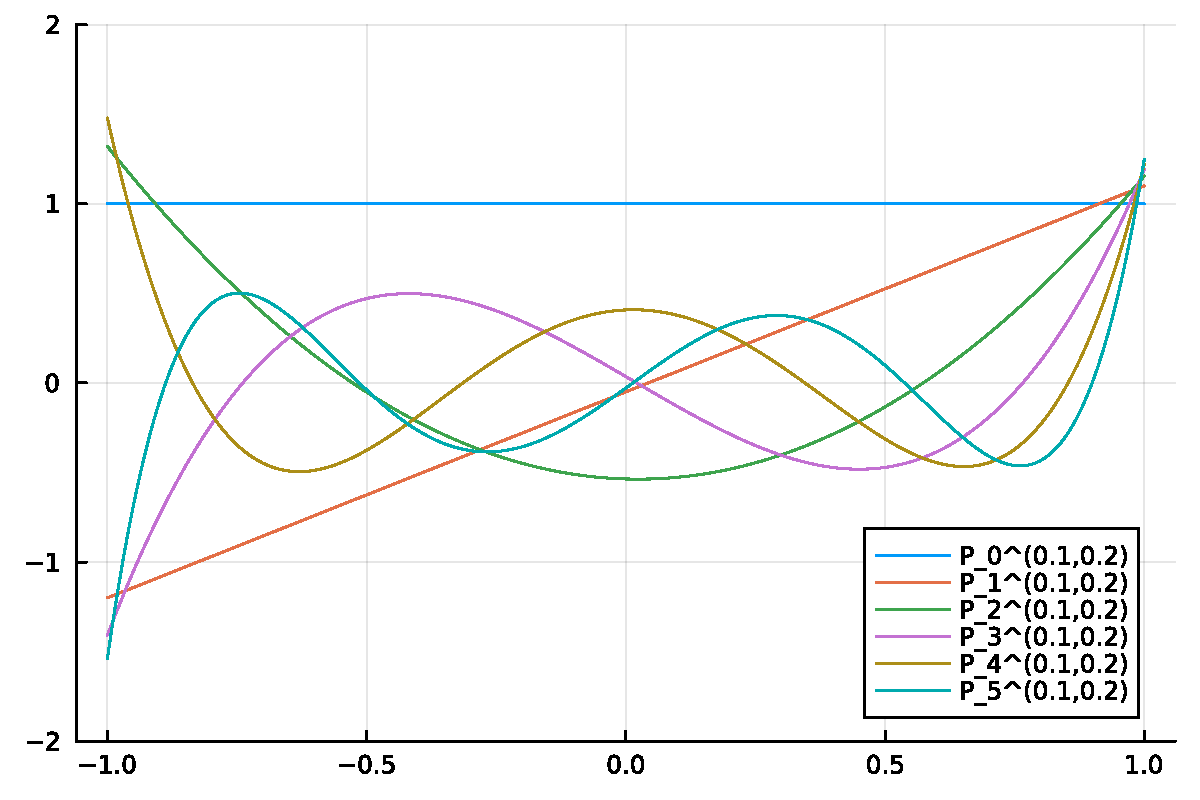
\includegraphics[width=\linewidth]{jl_dOthw0/OP_methods_12_1.pdf}

\begin{lstlisting}
(*@\HLJLn{w}@*) (*@\HLJLoB{=}@*) (*@\HLJLnf{Fun}@*)(*@\HLJLp{(}@*)(*@\HLJLnf{JacobiWeight}@*)(*@\HLJLp{(}@*)(*@\HLJLn{\ensuremath{\beta}}@*)(*@\HLJLp{,}@*)(*@\HLJLn{\ensuremath{\alpha}}@*)(*@\HLJLp{),}@*) (*@\HLJLp{[}@*)(*@\HLJLnfB{1.0}@*)(*@\HLJLp{])}@*)
(*@\HLJLnd{@show}@*) (*@\HLJLnf{sum}@*)(*@\HLJLp{(}@*)(*@\HLJLn{P\ensuremath{\_2}}@*)(*@\HLJLoB{*}@*)(*@\HLJLn{P\ensuremath{\_5}}@*)(*@\HLJLoB{*}@*)(*@\HLJLn{w}@*)(*@\HLJLp{)}@*)  (*@\HLJLcs{{\#}}@*) (*@\HLJLcs{means}@*) (*@\HLJLcs{integrate}@*)
(*@\HLJLnd{@show}@*) (*@\HLJLnf{sum}@*)(*@\HLJLp{(}@*)(*@\HLJLn{P\ensuremath{\_5}}@*)(*@\HLJLoB{*}@*)(*@\HLJLn{P\ensuremath{\_5}}@*)(*@\HLJLoB{*}@*)(*@\HLJLn{w}@*)(*@\HLJLp{);}@*)
\end{lstlisting}

\begin{lstlisting}
sum(P(*@\ensuremath{\_2}@*) * P(*@\ensuremath{\_5}@*) * w) = 1.0328132900334873e-17
sum(P(*@\ensuremath{\_5}@*) * P(*@\ensuremath{\_5}@*) * w) = 0.21713358248393153
\end{lstlisting}


\subsection{Legendre, Chebyshev, and ultraspherical polynomials}
There are special families of Jacobi weights with their own name.

\begin{tabular}
{l | l | l | l | l}
Name & Jacobi parameters & $w(x)$ & Notation & $k_n$ \\
\hline
Jacobi & $\alpha,\beta$ & $(1-x)^{\alpha} (1+x)^\beta$ & $P_n^{(\alpha,\beta)}(x)$ & \href{http://dlmf.nist.gov/18.3}{Table 18.3.1} \\
Legendre & $0,0$ & $1$ & $P_n(x)$ & $2^n(1/2)_n/n!$ \\
Chebyshev (1st) & $-{1 \over 2},-{1 \over 2}$ & $1 \over \sqrt{1-x^2}$ & $T_n(x)$ & $1 (n=0), 2^{n-1} (n \neq 0)$ \\
Chebyshev (2nd) & ${1 \over 2},{1 \over 2}$ & $\sqrt{1-x^2}$ & $U_n(x)$ & $2^n$ \\
Ultraspherical & $\lambda-{1 \over 2},\lambda-{1 \over 2}$ & $(1-x^2)^{\lambda - 1/2}, \lambda \neq 0$ & $C_n^{(\lambda)}(x)$ & $2^n(\lambda)_n/n!$ \\
\end{tabular}
Note that other than Legendre, these polynomials have a different normalization than $P_n^{(\alpha,\beta)}$:


\begin{lstlisting}
(*@\HLJLn{T\ensuremath{\_2}}@*) (*@\HLJLoB{=}@*) (*@\HLJLnf{Fun}@*)(*@\HLJLp{(}@*)(*@\HLJLnf{Chebyshev}@*)(*@\HLJLp{(),}@*) (*@\HLJLp{[}@*)(*@\HLJLnfB{0.0}@*)(*@\HLJLp{,}@*)(*@\HLJLni{0}@*)(*@\HLJLp{,}@*)(*@\HLJLni{1}@*)(*@\HLJLp{])}@*)
(*@\HLJLn{P\ensuremath{\_2}}@*) (*@\HLJLoB{=}@*) (*@\HLJLnf{Fun}@*)(*@\HLJLp{(}@*)(*@\HLJLnf{Jacobi}@*)(*@\HLJLp{(}@*)(*@\HLJLoB{-}@*)(*@\HLJLni{1}@*)(*@\HLJLoB{/}@*)(*@\HLJLni{2}@*)(*@\HLJLp{,}@*)(*@\HLJLoB{-}@*)(*@\HLJLni{1}@*)(*@\HLJLoB{/}@*)(*@\HLJLni{2}@*)(*@\HLJLp{),}@*) (*@\HLJLp{[}@*)(*@\HLJLnfB{0.0}@*)(*@\HLJLp{,}@*)(*@\HLJLni{0}@*)(*@\HLJLp{,}@*)(*@\HLJLni{1}@*)(*@\HLJLp{])}@*)
(*@\HLJLnf{plot}@*)(*@\HLJLp{(}@*)(*@\HLJLn{T\ensuremath{\_2}}@*)(*@\HLJLp{;}@*) (*@\HLJLn{label}@*)(*@\HLJLoB{=}@*)(*@\HLJLs{"{}T{\_}2"{}}@*)(*@\HLJLp{,}@*) (*@\HLJLn{title}@*)(*@\HLJLoB{=}@*)(*@\HLJLs{"{}T{\_}2}@*) (*@\HLJLs{is}@*) (*@\HLJLs{C*P{\_}2}@*) (*@\HLJLs{for}@*) (*@\HLJLs{some}@*) (*@\HLJLs{C"{}}@*)(*@\HLJLp{)}@*)
(*@\HLJLnf{plot!}@*)(*@\HLJLp{(}@*)(*@\HLJLn{P\ensuremath{\_2}}@*)(*@\HLJLp{;}@*) (*@\HLJLn{label}@*)(*@\HLJLoB{=}@*)(*@\HLJLs{"{}P{\_}2"{}}@*)(*@\HLJLp{)}@*)
\end{lstlisting}

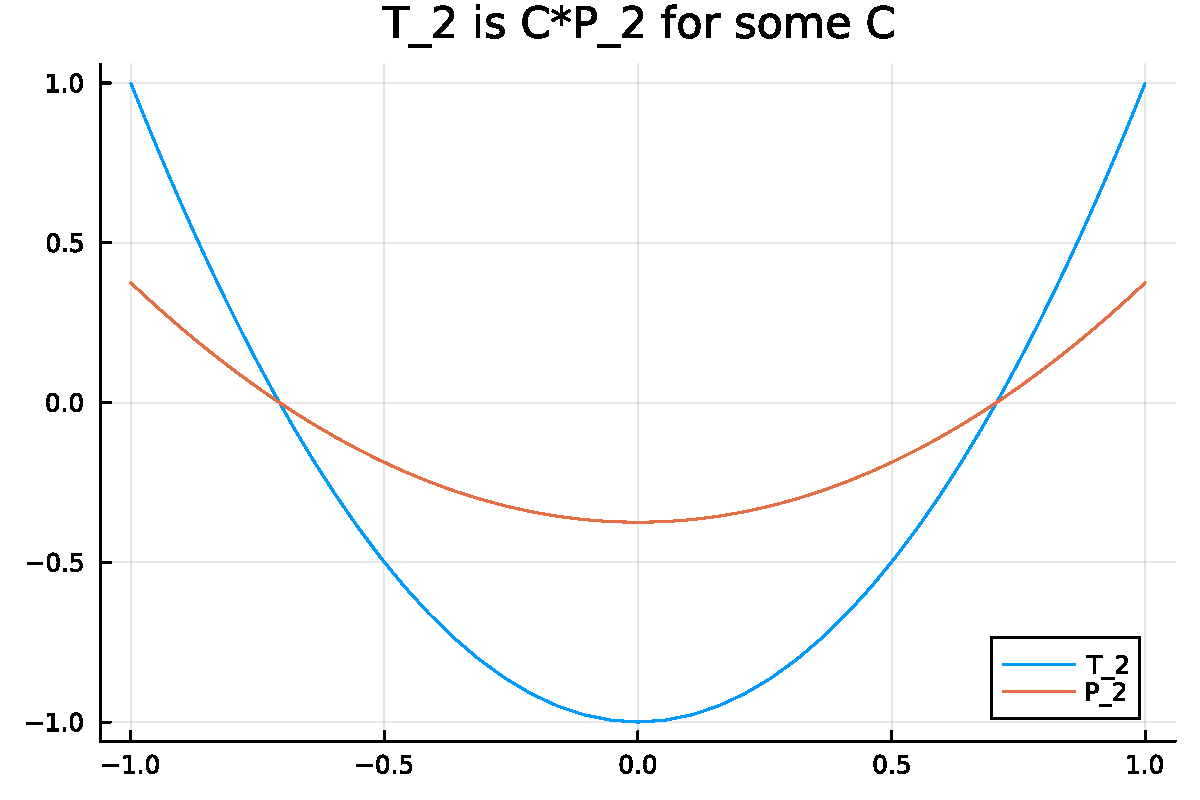
\includegraphics[width=\linewidth]{jl_dOthw0/OP_methods_14_1.pdf}

But because they are orthogonal w.r.t. the same weight, they must be a constant multiple of each-other, as discussed last lecture.

\subsubsection{Explicit construction of Chebyshev polynomials (first kind and second kind)}
Chebyshev polynomials are pretty much the only OPs with \emph{simple} closed form expressions.

\textbf{Proposition (Chebyshev first kind formula)} $T_n(x) = \cos n\, {\rm acos} x$ or in other words,

\[
T_n(\cos \theta) = \cos n \theta
\]
\textbf{Proof} We first show that they are orthogonal w.r.t. $1/\sqrt{1-x^2}$. Too easy: do $x = \cos \theta$, ${\rm d}x = -\sin \theta {\rm d}\theta$ to get (for $n \neq m$)


\begin{align*}
    \int_{-1}^1 {\cos n\, {\rm acos}x \cos m \, {\rm acos}x  {\rm d}x \over \sqrt{1-x^2}} &= -\int_\pi^0  \cos n \theta \cos m \theta {\rm d} \theta 
    =  \int_0^\pi  {{\rm e}^{{\rm i} (-n-m)\theta} + {\rm e}^{{\rm i} (n-m)\theta} + {\rm e}^{{\rm i} (m-n)\theta} + {\rm e}^{{\rm i} (n+m)\theta}    \over 4} {\rm d} \theta =0
\end{align*}
We then need to show it has the right highest order term $k_n$. Note that $k_0 = k_1 = 1$.  Using $z = {\rm e}^{{\rm i} \theta}$ we see that $\cos n \theta$ has a simple recurrence for $n=2,3,\ldots$:

\[
\cos n \theta = {z^n + z^{-n} \over 2} = 2 {z + z^{-1} \over 2} {z^{n-1} + z^{1-n} \over 2}- {z^{n-2} + z^{2-n} \over 2} =
2 \cos \theta \cos (n-1)\theta - \cos(n-2)\theta
\]
thus

\[
\cos n\, {\rm acos}x = 2 x \cos(n-1) \, {\rm acos}x - \cos(n-2)\, {\rm acos}x
\]
It follows that

\[
k_n = 2  k_{n-1} = 2^{n-1} k_1 = 2^{n-1}
\]
By uniqueness we have $T_n(x) = \cos n\, {\rm acos}x$.

\[
\blacksquare
\]
\textbf{Proposition (Chebyshev second kind formula)} $U_n(x) = {\sin (n+1) \, {\rm acos} x \over \sin \, {\rm acos} x}$ or in other words,

\[
U_n(\cos \theta) = {\sin (n+1) \theta \over \sin \theta}
\]
\emph{Example} For the case of Chebyshev polynomials, we have

\[
J = \begin{pmatrix}
0 & 1 \cr
{1\over 2} & 0 & {1\over 2}\cr
& {1\over 2} & 0 & {1\over 2} \cr
&& {1\over 2} & 0 & \ddots \cr
&&&\ddots & \ddots
\end{pmatrix}
\]
Therefore, the Chebyshev coefficients of $x f(x)$ are given by

\[
J^\top \mathbf{f} = \begin{pmatrix}
0 & {1\over 2} \cr
1 & 0 & {1\over 2} \cr
& {1\over 2} & 0 & {1\over 2} \cr
&& {1\over 2} & 0 & \ddots \cr
&&&\ddots & \ddots
\end{pmatrix} \begin{pmatrix} f_0\\ f_1\\f_2\\f_3\\\vdots\end{pmatrix}
\]
\subsubsection{Demonstration}
In the case where $f$ is a degree $n-1$  polynomial, we can represent $J^\top$ as an $n+1 \times n$ matrix (this makes sense as $x f(x)$ is one more degree than $f$):


\begin{lstlisting}
(*@\HLJLn{f}@*) (*@\HLJLoB{=}@*) (*@\HLJLnf{Fun}@*)(*@\HLJLp{(}@*)(*@\HLJLn{exp}@*)(*@\HLJLp{,}@*) (*@\HLJLnf{Chebyshev}@*)(*@\HLJLp{())}@*)
(*@\HLJLn{n}@*) (*@\HLJLoB{=}@*) (*@\HLJLnf{ncoefficients}@*)(*@\HLJLp{(}@*)(*@\HLJLn{f}@*)(*@\HLJLp{)}@*) (*@\HLJLcs{{\#}}@*) (*@\HLJLcs{number}@*) (*@\HLJLcs{of}@*) (*@\HLJLcs{coefficients}@*)
(*@\HLJLnd{@show}@*) (*@\HLJLn{n}@*)
(*@\HLJLn{J}@*) (*@\HLJLoB{=}@*) (*@\HLJLnf{zeros}@*)(*@\HLJLp{(}@*)(*@\HLJLn{n}@*)(*@\HLJLp{,}@*)(*@\HLJLn{n}@*)(*@\HLJLoB{+}@*)(*@\HLJLni{1}@*)(*@\HLJLp{)}@*)
(*@\HLJLn{J}@*)(*@\HLJLp{[}@*)(*@\HLJLni{1}@*)(*@\HLJLp{,}@*)(*@\HLJLni{2}@*)(*@\HLJLp{]}@*) (*@\HLJLoB{=}@*) (*@\HLJLni{1}@*)
(*@\HLJLk{for}@*) (*@\HLJLn{k}@*)(*@\HLJLoB{=}@*)(*@\HLJLni{2}@*)(*@\HLJLoB{:}@*)(*@\HLJLn{n}@*)
    (*@\HLJLn{J}@*)(*@\HLJLp{[}@*)(*@\HLJLn{k}@*)(*@\HLJLp{,}@*)(*@\HLJLn{k}@*)(*@\HLJLoB{-}@*)(*@\HLJLni{1}@*)(*@\HLJLp{]}@*) (*@\HLJLoB{=}@*) (*@\HLJLn{J}@*)(*@\HLJLp{[}@*)(*@\HLJLn{k}@*)(*@\HLJLp{,}@*)(*@\HLJLn{k}@*)(*@\HLJLoB{+}@*)(*@\HLJLni{1}@*)(*@\HLJLp{]}@*) (*@\HLJLoB{=}@*) (*@\HLJLni{1}@*)(*@\HLJLoB{/}@*)(*@\HLJLni{2}@*)
(*@\HLJLk{end}@*)
(*@\HLJLn{J}@*)(*@\HLJLoB{{\textquotesingle}}@*)
\end{lstlisting}

\begin{lstlisting}
n = 14
15(*@\ensuremath{\times}@*)14 adjoint(::Matrix(*@{{\{}}@*)Float64(*@{{\}}}@*)) with eltype Float64:
 0.0  0.5  0.0  0.0  0.0  0.0  0.0  0.0  0.0  0.0  0.0  0.0  0.0  0.0
 1.0  0.0  0.5  0.0  0.0  0.0  0.0  0.0  0.0  0.0  0.0  0.0  0.0  0.0
 0.0  0.5  0.0  0.5  0.0  0.0  0.0  0.0  0.0  0.0  0.0  0.0  0.0  0.0
 0.0  0.0  0.5  0.0  0.5  0.0  0.0  0.0  0.0  0.0  0.0  0.0  0.0  0.0
 0.0  0.0  0.0  0.5  0.0  0.5  0.0  0.0  0.0  0.0  0.0  0.0  0.0  0.0
 0.0  0.0  0.0  0.0  0.5  0.0  0.5  0.0  0.0  0.0  0.0  0.0  0.0  0.0
 0.0  0.0  0.0  0.0  0.0  0.5  0.0  0.5  0.0  0.0  0.0  0.0  0.0  0.0
 0.0  0.0  0.0  0.0  0.0  0.0  0.5  0.0  0.5  0.0  0.0  0.0  0.0  0.0
 0.0  0.0  0.0  0.0  0.0  0.0  0.0  0.5  0.0  0.5  0.0  0.0  0.0  0.0
 0.0  0.0  0.0  0.0  0.0  0.0  0.0  0.0  0.5  0.0  0.5  0.0  0.0  0.0
 0.0  0.0  0.0  0.0  0.0  0.0  0.0  0.0  0.0  0.5  0.0  0.5  0.0  0.0
 0.0  0.0  0.0  0.0  0.0  0.0  0.0  0.0  0.0  0.0  0.5  0.0  0.5  0.0
 0.0  0.0  0.0  0.0  0.0  0.0  0.0  0.0  0.0  0.0  0.0  0.5  0.0  0.5
 0.0  0.0  0.0  0.0  0.0  0.0  0.0  0.0  0.0  0.0  0.0  0.0  0.5  0.0
 0.0  0.0  0.0  0.0  0.0  0.0  0.0  0.0  0.0  0.0  0.0  0.0  0.0  0.5
\end{lstlisting}


\begin{lstlisting}
(*@\HLJLn{cfs}@*) (*@\HLJLoB{=}@*) (*@\HLJLn{J}@*)(*@\HLJLoB{{\textquotesingle}*}@*)(*@\HLJLn{f}@*)(*@\HLJLoB{.}@*)(*@\HLJLn{coefficients}@*) (*@\HLJLcs{{\#}}@*) (*@\HLJLcs{coefficients}@*) (*@\HLJLcs{of}@*) (*@\HLJLcs{x*f}@*)
(*@\HLJLn{xf}@*) (*@\HLJLoB{=}@*) (*@\HLJLnf{Fun}@*)(*@\HLJLp{(}@*)(*@\HLJLnf{Chebyshev}@*)(*@\HLJLp{(),}@*) (*@\HLJLn{cfs}@*)(*@\HLJLp{)}@*)

(*@\HLJLnf{xf}@*)(*@\HLJLp{(}@*)(*@\HLJLnfB{0.1}@*)(*@\HLJLp{)}@*) (*@\HLJLoB{-}@*) (*@\HLJLnfB{0.1}@*)(*@\HLJLoB{*}@*)(*@\HLJLnf{f}@*)(*@\HLJLp{(}@*)(*@\HLJLnfB{0.1}@*)(*@\HLJLp{)}@*)
\end{lstlisting}

\begin{lstlisting}
-6.938893903907228e-17
\end{lstlisting}


We can construct $T_0(x),\ldots,T_{n-1}(x)$ via


\begin{align*}
    T_0(x) &= 1\\
    T_1(x) &= x T_0(x) \\
    T_{k+1}(x) &= 2x  T_k(x) -  T_{k-1}(x), \qquad 1 \leq k \leq n-2
\end{align*}
Believe it or not, this is much faster than using $\cos k\, {\rm acos} x$:


\begin{lstlisting}
(*@\HLJLk{function}@*) (*@\HLJLnf{recurrence{\_}Chebyshev}@*)(*@\HLJLp{(}@*)(*@\HLJLn{n}@*)(*@\HLJLp{,}@*)(*@\HLJLn{x}@*)(*@\HLJLp{)}@*)
    (*@\HLJLn{T}@*) (*@\HLJLoB{=}@*) (*@\HLJLnf{zeros}@*)(*@\HLJLp{(}@*)(*@\HLJLn{n}@*)(*@\HLJLp{)}@*)
    (*@\HLJLn{T}@*)(*@\HLJLp{[}@*)(*@\HLJLni{1}@*)(*@\HLJLp{]}@*) (*@\HLJLoB{=}@*) (*@\HLJLnfB{1.0}@*)
    (*@\HLJLn{T}@*)(*@\HLJLp{[}@*)(*@\HLJLni{2}@*)(*@\HLJLp{]}@*) (*@\HLJLoB{=}@*) (*@\HLJLn{x}@*)(*@\HLJLoB{*}@*)(*@\HLJLn{T}@*)(*@\HLJLp{[}@*)(*@\HLJLni{1}@*)(*@\HLJLp{]}@*)
    (*@\HLJLk{for}@*) (*@\HLJLn{k}@*) (*@\HLJLoB{=}@*) (*@\HLJLni{2}@*)(*@\HLJLoB{:}@*)(*@\HLJLn{n}@*)(*@\HLJLoB{-}@*)(*@\HLJLni{1}@*)
        (*@\HLJLn{T}@*)(*@\HLJLp{[}@*)(*@\HLJLn{k}@*)(*@\HLJLoB{+}@*)(*@\HLJLni{1}@*)(*@\HLJLp{]}@*) (*@\HLJLoB{=}@*) (*@\HLJLni{2}@*)(*@\HLJLn{x}@*)(*@\HLJLoB{*}@*)(*@\HLJLn{T}@*)(*@\HLJLp{[}@*)(*@\HLJLn{k}@*)(*@\HLJLp{]}@*) (*@\HLJLoB{-}@*) (*@\HLJLn{T}@*)(*@\HLJLp{[}@*)(*@\HLJLn{k}@*)(*@\HLJLoB{-}@*)(*@\HLJLni{1}@*)(*@\HLJLp{]}@*)
    (*@\HLJLk{end}@*)
    (*@\HLJLn{T}@*)
(*@\HLJLk{end}@*)

(*@\HLJLnf{trig{\_}Chebyshev}@*)(*@\HLJLp{(}@*)(*@\HLJLn{n}@*)(*@\HLJLp{,}@*)(*@\HLJLn{x}@*)(*@\HLJLp{)}@*) (*@\HLJLoB{=}@*) (*@\HLJLp{[}@*)(*@\HLJLnf{cos}@*)(*@\HLJLp{(}@*)(*@\HLJLn{k}@*)(*@\HLJLoB{*}@*)(*@\HLJLnf{acos}@*)(*@\HLJLp{(}@*)(*@\HLJLn{x}@*)(*@\HLJLp{))}@*) (*@\HLJLk{for}@*) (*@\HLJLn{k}@*)(*@\HLJLoB{=}@*)(*@\HLJLni{0}@*)(*@\HLJLoB{:}@*)(*@\HLJLn{n}@*)(*@\HLJLoB{-}@*)(*@\HLJLni{1}@*)(*@\HLJLp{]}@*)

(*@\HLJLn{n}@*) (*@\HLJLoB{=}@*) (*@\HLJLni{10}@*)
(*@\HLJLnf{recurrence{\_}Chebyshev}@*)(*@\HLJLp{(}@*)(*@\HLJLn{n}@*)(*@\HLJLp{,}@*) (*@\HLJLnfB{0.1}@*)(*@\HLJLp{)}@*) (*@\HLJLoB{-}@*) (*@\HLJLnf{trig{\_}Chebyshev}@*)(*@\HLJLp{(}@*)(*@\HLJLn{n}@*)(*@\HLJLp{,}@*)(*@\HLJLnfB{0.1}@*)(*@\HLJLp{)}@*) (*@\HLJLoB{|>}@*)(*@\HLJLn{norm}@*)
\end{lstlisting}

\begin{lstlisting}
1.1102230246251565e-16
\end{lstlisting}


\begin{lstlisting}
(*@\HLJLn{n}@*) (*@\HLJLoB{=}@*) (*@\HLJLni{10000}@*)
(*@\HLJLnd{@time}@*) (*@\HLJLnf{recurrence{\_}Chebyshev}@*)(*@\HLJLp{(}@*)(*@\HLJLn{n}@*)(*@\HLJLp{,}@*) (*@\HLJLnfB{0.1}@*)(*@\HLJLp{)}@*)
(*@\HLJLnd{@time}@*) (*@\HLJLnf{trig{\_}Chebyshev}@*)(*@\HLJLp{(}@*)(*@\HLJLn{n}@*)(*@\HLJLp{,}@*)(*@\HLJLnfB{0.1}@*)(*@\HLJLp{);}@*)
\end{lstlisting}

\begin{lstlisting}
0.000041 seconds (2 allocations: 78.172 KiB)
  0.000339 seconds (2 allocations: 78.172 KiB)
\end{lstlisting}


We can also demonstrate Clenshaw's algorithm for evaluating polynomials. To evaluate an expansion in Chebyshev polynomials,

\[
\sum_{k = 0}^{n-1}f_kT_k(x)
\]
we want to solve the system

\[
\underbrace{\begin{pmatrix}
1 & -x & {1\over 2} \\
& 1 & -x & {1\over 2}  \\
& & {1\over 2} & -x & \ddots  \\
& &     & {1\over 2} & \ddots & {1\over 2} \\
&&&&\ddots & -x \\
&&&&& {1\over 2}
\end{pmatrix}}_{L_x^\top} \begin{pmatrix} \gamma_0 \\\vdots\\ \gamma_{n-1} \end{pmatrix}
\]
via


\begin{align*}
\gamma_{n-1} &= 2f_{n-1} \\
\gamma_{n-2} &= 2f_{n-2} + 2x \gamma_{n-1} \\
\gamma_{n-3} &= 2 f_{n-3} + 2x \gamma_{n-2} - \gamma_{n-1} \\
& \vdots \\
\gamma_1 &= f_1 + x \gamma_2 - {1\over 2} \gamma_3 \\
\gamma_0 &= f_0 + x \gamma_1 - {1\over 2} \gamma_2
\end{align*}
then $f(x) = \gamma_0$.


\begin{lstlisting}
(*@\HLJLk{function}@*) (*@\HLJLnf{clenshaw{\_}Chebyshev}@*)(*@\HLJLp{(}@*)(*@\HLJLn{f}@*)(*@\HLJLp{,}@*)(*@\HLJLn{x}@*)(*@\HLJLp{)}@*)
    (*@\HLJLn{n}@*) (*@\HLJLoB{=}@*) (*@\HLJLnf{length}@*)(*@\HLJLp{(}@*)(*@\HLJLn{f}@*)(*@\HLJLp{)}@*)
    (*@\HLJLn{\ensuremath{\gamma}}@*) (*@\HLJLoB{=}@*) (*@\HLJLnf{zeros}@*)(*@\HLJLp{(}@*)(*@\HLJLn{n}@*)(*@\HLJLp{)}@*)
    (*@\HLJLn{\ensuremath{\gamma}}@*)(*@\HLJLp{[}@*)(*@\HLJLn{n}@*)(*@\HLJLp{]}@*) (*@\HLJLoB{=}@*) (*@\HLJLni{2}@*)(*@\HLJLn{f}@*)(*@\HLJLp{[}@*)(*@\HLJLn{n}@*)(*@\HLJLp{]}@*)
    (*@\HLJLn{\ensuremath{\gamma}}@*)(*@\HLJLp{[}@*)(*@\HLJLn{n}@*)(*@\HLJLoB{-}@*)(*@\HLJLni{1}@*)(*@\HLJLp{]}@*) (*@\HLJLoB{=}@*) (*@\HLJLni{2}@*)(*@\HLJLn{f}@*)(*@\HLJLp{[}@*)(*@\HLJLn{n}@*)(*@\HLJLoB{-}@*)(*@\HLJLni{1}@*)(*@\HLJLp{]}@*) (*@\HLJLoB{+}@*)(*@\HLJLni{2}@*)(*@\HLJLn{x}@*)(*@\HLJLoB{*}@*)(*@\HLJLn{f}@*)(*@\HLJLp{[}@*)(*@\HLJLn{n}@*)(*@\HLJLp{]}@*)
    (*@\HLJLk{for}@*) (*@\HLJLn{k}@*) (*@\HLJLoB{=}@*) (*@\HLJLn{n}@*)(*@\HLJLoB{-}@*)(*@\HLJLni{2}@*)(*@\HLJLoB{:-}@*)(*@\HLJLni{1}@*)(*@\HLJLoB{:}@*)(*@\HLJLni{1}@*)
        (*@\HLJLn{\ensuremath{\gamma}}@*)(*@\HLJLp{[}@*)(*@\HLJLn{k}@*)(*@\HLJLp{]}@*) (*@\HLJLoB{=}@*) (*@\HLJLni{2}@*)(*@\HLJLn{f}@*)(*@\HLJLp{[}@*)(*@\HLJLn{k}@*)(*@\HLJLp{]}@*) (*@\HLJLoB{+}@*) (*@\HLJLni{2}@*)(*@\HLJLn{x}@*)(*@\HLJLoB{*}@*)(*@\HLJLn{\ensuremath{\gamma}}@*)(*@\HLJLp{[}@*)(*@\HLJLn{k}@*)(*@\HLJLoB{+}@*)(*@\HLJLni{1}@*)(*@\HLJLp{]}@*) (*@\HLJLoB{-}@*) (*@\HLJLn{\ensuremath{\gamma}}@*)(*@\HLJLp{[}@*)(*@\HLJLn{k}@*)(*@\HLJLoB{+}@*)(*@\HLJLni{2}@*)(*@\HLJLp{]}@*)
    (*@\HLJLk{end}@*)
    (*@\HLJLn{\ensuremath{\gamma}}@*)(*@\HLJLp{[}@*)(*@\HLJLni{2}@*)(*@\HLJLp{]}@*) (*@\HLJLoB{=}@*) (*@\HLJLn{f}@*)(*@\HLJLp{[}@*)(*@\HLJLni{2}@*)(*@\HLJLp{]}@*) (*@\HLJLoB{+}@*) (*@\HLJLn{x}@*)(*@\HLJLoB{*}@*)(*@\HLJLn{\ensuremath{\gamma}}@*)(*@\HLJLp{[}@*)(*@\HLJLni{3}@*)(*@\HLJLp{]}@*) (*@\HLJLoB{-}@*) (*@\HLJLn{\ensuremath{\gamma}}@*)(*@\HLJLp{[}@*)(*@\HLJLni{4}@*)(*@\HLJLp{]}@*)(*@\HLJLoB{/}@*)(*@\HLJLni{2}@*)
    (*@\HLJLn{\ensuremath{\gamma}}@*)(*@\HLJLp{[}@*)(*@\HLJLni{1}@*)(*@\HLJLp{]}@*) (*@\HLJLoB{=}@*) (*@\HLJLn{f}@*)(*@\HLJLp{[}@*)(*@\HLJLni{1}@*)(*@\HLJLp{]}@*) (*@\HLJLoB{+}@*) (*@\HLJLn{x}@*)(*@\HLJLoB{*}@*)(*@\HLJLn{\ensuremath{\gamma}}@*)(*@\HLJLp{[}@*)(*@\HLJLni{2}@*)(*@\HLJLp{]}@*) (*@\HLJLoB{-}@*) (*@\HLJLn{\ensuremath{\gamma}}@*)(*@\HLJLp{[}@*)(*@\HLJLni{3}@*)(*@\HLJLp{]}@*)(*@\HLJLoB{/}@*)(*@\HLJLni{2}@*)
    (*@\HLJLn{\ensuremath{\gamma}}@*)(*@\HLJLp{[}@*)(*@\HLJLni{1}@*)(*@\HLJLp{]}@*)
(*@\HLJLk{end}@*)

(*@\HLJLn{f}@*) (*@\HLJLoB{=}@*) (*@\HLJLnf{Fun}@*)(*@\HLJLp{(}@*)(*@\HLJLn{exp}@*)(*@\HLJLp{,}@*) (*@\HLJLnf{Chebyshev}@*)(*@\HLJLp{())}@*)
(*@\HLJLnf{clenshaw{\_}Chebyshev}@*)(*@\HLJLp{(}@*)(*@\HLJLn{f}@*)(*@\HLJLoB{.}@*)(*@\HLJLn{coefficients}@*)(*@\HLJLp{,}@*) (*@\HLJLnfB{0.1}@*)(*@\HLJLp{)}@*) (*@\HLJLoB{-}@*) (*@\HLJLnf{exp}@*)(*@\HLJLp{(}@*)(*@\HLJLnfB{0.1}@*)(*@\HLJLp{)}@*)
\end{lstlisting}

\begin{lstlisting}
-1.3322676295501878e-15
\end{lstlisting}


With some high performance computing tweaks, this can be made more accurate. This is the algorithm used for evaluating functions in ApproxFun:


\begin{lstlisting}
(*@\HLJLnf{f}@*)(*@\HLJLp{(}@*)(*@\HLJLnfB{0.1}@*)(*@\HLJLp{)}@*) (*@\HLJLoB{-}@*) (*@\HLJLnf{exp}@*)(*@\HLJLp{(}@*)(*@\HLJLnfB{0.1}@*)(*@\HLJLp{)}@*)
\end{lstlisting}

\begin{lstlisting}
0.0
\end{lstlisting}


\section{Interpolation and Gaussian quadrature}
\emph{Polynomial interpolation} is the process of finding a polynomial that equals data at a precise set of points. \emph{Quadrature} is the act of approximating an integral by a weighted sum:

\[
\int_a^b f(x) w(x) {\rm d}x \ensuremath{\approx} \sum_{j=1}^n w_j f(x_j).
\]
In these notes we see that the two concepts are intrinsically linked:  interpolation leads naturally to quadrature rules. Moreover, by using a set of points $x_j$ linked to orthogonal polynomials we get significantly more accurate rules, and in fact can use quadrature to compute expansions in orthogonal polynomials that interpolate. That is, we can mirror the link between the Trapezium rule, Fourier series, and interpolation but now for polynomials.

\begin{itemize}
\item[1. ] Polynomial Interpolation: we describe how to interpolate a function by a polynomial.


\item[2. ] Truncated Jacobi matrices: we see that truncated Jacobi matrices are diagonalisable

\end{itemize}
in terms of orthogonal polynomials and their zeros. 

\begin{itemize}
\item[2. ] Interpolatory quadrature rule: polynomial interpolation leads naturally to ways to integrate

\end{itemize}
functions, but onely realisable in the simplest cases.

\begin{itemize}
\item[3. ] Gaussian quadrature: Using roots of orthogonal polynomials and truncated Jacobi matrices 

\end{itemize}
leads naturally to an efficiently computable interpolatory quadrature rule. The \emph{miracle} is its exact for twice as many polynomials as expected.

\subsection{1. Polynomial Interpolation}
We already saw a special case of polynomial interpolation, where we saw that the polynomial

\[
f(z) \ensuremath{\approx} \ensuremath{\sum}_{k=0}^{n-1} \hat{f}_k^n z^k
\]
equaled $f$ at evenly spaced points on the unit circle: ${\rm e}^{{\rm i} 2\ensuremath{\pi} j/n}$.  But here we consider the following:

\textbf{Definition (interpolatory polynomial)} Given $n$ distinct points $x_1,\ensuremath{\ldots},x_n \ensuremath{\in} \ensuremath{\bbR}$  and $n$ \emph{samples} $f_1,\ensuremath{\ldots},f_n \ensuremath{\in} \ensuremath{\bbR}$, a degree $n-1$ \emph{interpolatory polynomial} $p(x)$ satisfies

\[
p(x_j) = f_j
\]
The easiest way to solve this problem is to invert the Vandermonde system:

\textbf{Definition (Vandermonde)} The \emph{Vandermonde matrix} associated with $n$ distinct points $x_1,\ensuremath{\ldots},x_n \ensuremath{\in} \ensuremath{\bbR}$ is the matrix

\[
V := \begin{bmatrix} 1 & x_1 & \ensuremath{\cdots} & x_1^{n-1} \\
                    \ensuremath{\vdots} & \ensuremath{\vdots} & \ensuremath{\ddots} & \ensuremath{\vdots} \\
                    1 & x_n & \ensuremath{\cdots} & x_n^{n-1}
                    \end{bmatrix}
\]
\textbf{Proposition (interpolatory polynomial uniqueness)}  The interpolatory polynomial is unique, and the Vandermonde matrix is invertible.

\textbf{Proof} Suppose $p$ and $\tilde{p}$ are both interpolatory polynomials. Then $p(x) - \tilde{p}(x)$ vanishes at $n$ distinct points $x_j$. By the fundamental theorem of algebra it must be zero, i.e., $p = \tilde{p}$.

For the second part, if $V \mathbf{c} = 0$ for $\mathbf{c} \ensuremath{\in} \ensuremath{\bbR}$ then for $q(x) = c_1 + \ensuremath{\cdots} + c_n x^{n-1}$ we have

\[
q(x_j) = \mathbf{e}_j^\ensuremath{\top} V \mathbf{c} = 0
\]
hence $q$ vanishes at $n$ distinct points and is therefore 0, i.e., $\mathbf{c} = 0$. $\blacksquare$

Thus a quick-and-dirty way to to do interpolation is to invert the Vandermonde matrix (which we saw in the least squares setting with more samples then coefficients):


\begin{lstlisting}
(*@\HLJLk{using}@*) (*@\HLJLn{Plots}@*)(*@\HLJLp{,}@*) (*@\HLJLn{LinearAlgebra}@*)
(*@\HLJLn{f}@*) (*@\HLJLoB{=}@*) (*@\HLJLn{x}@*) (*@\HLJLoB{->}@*) (*@\HLJLnf{cos}@*)(*@\HLJLp{(}@*)(*@\HLJLni{10}@*)(*@\HLJLn{x}@*)(*@\HLJLp{)}@*)
(*@\HLJLn{n}@*) (*@\HLJLoB{=}@*) (*@\HLJLni{5}@*)

(*@\HLJLn{x}@*) (*@\HLJLoB{=}@*) (*@\HLJLnf{range}@*)(*@\HLJLp{(}@*)(*@\HLJLni{0}@*)(*@\HLJLp{,}@*) (*@\HLJLni{1}@*)(*@\HLJLp{;}@*) (*@\HLJLn{length}@*)(*@\HLJLoB{=}@*)(*@\HLJLn{n}@*)(*@\HLJLp{)}@*)(*@\HLJLcs{{\#}}@*) (*@\HLJLcs{evenly}@*) (*@\HLJLcs{spaced}@*) (*@\HLJLcs{points}@*) (*@\HLJLcs{(BAD}@*) (*@\HLJLcs{for}@*) (*@\HLJLcs{interpolation)}@*)
(*@\HLJLn{V}@*) (*@\HLJLoB{=}@*) (*@\HLJLn{x}@*) (*@\HLJLoB{.{\textasciicircum}}@*) (*@\HLJLp{(}@*)(*@\HLJLni{0}@*)(*@\HLJLoB{:}@*)(*@\HLJLn{n}@*)(*@\HLJLoB{-}@*)(*@\HLJLni{1}@*)(*@\HLJLp{)}@*)(*@\HLJLoB{{\textquotesingle}}@*) (*@\HLJLcs{{\#}}@*) (*@\HLJLcs{Vandermonde}@*) (*@\HLJLcs{matrix}@*)
(*@\HLJLn{c}@*) (*@\HLJLoB{=}@*) (*@\HLJLn{V}@*) (*@\HLJLoB{{\textbackslash}}@*) (*@\HLJLn{f}@*)(*@\HLJLoB{.}@*)(*@\HLJLp{(}@*)(*@\HLJLn{x}@*)(*@\HLJLp{)}@*) (*@\HLJLcs{{\#}}@*) (*@\HLJLcs{coefficients}@*) (*@\HLJLcs{of}@*) (*@\HLJLcs{interpolatory}@*) (*@\HLJLcs{polynomial}@*)
(*@\HLJLn{p}@*) (*@\HLJLoB{=}@*) (*@\HLJLn{x}@*) (*@\HLJLoB{->}@*) (*@\HLJLnf{dot}@*)(*@\HLJLp{(}@*)(*@\HLJLn{c}@*)(*@\HLJLp{,}@*) (*@\HLJLn{x}@*) (*@\HLJLoB{.{\textasciicircum}}@*) (*@\HLJLp{(}@*)(*@\HLJLni{0}@*)(*@\HLJLoB{:}@*)(*@\HLJLn{n}@*)(*@\HLJLoB{-}@*)(*@\HLJLni{1}@*)(*@\HLJLp{))}@*)

(*@\HLJLn{g}@*) (*@\HLJLoB{=}@*) (*@\HLJLnf{range}@*)(*@\HLJLp{(}@*)(*@\HLJLni{0}@*)(*@\HLJLp{,}@*)(*@\HLJLni{1}@*)(*@\HLJLp{;}@*) (*@\HLJLn{length}@*)(*@\HLJLoB{=}@*)(*@\HLJLni{1000}@*)(*@\HLJLp{)}@*) (*@\HLJLcs{{\#}}@*) (*@\HLJLcs{plotting}@*) (*@\HLJLcs{grid}@*)
(*@\HLJLnf{plot}@*)(*@\HLJLp{(}@*)(*@\HLJLn{g}@*)(*@\HLJLp{,}@*) (*@\HLJLn{f}@*)(*@\HLJLoB{.}@*)(*@\HLJLp{(}@*)(*@\HLJLn{g}@*)(*@\HLJLp{);}@*) (*@\HLJLn{label}@*)(*@\HLJLoB{=}@*)(*@\HLJLs{"{}function"{}}@*)(*@\HLJLp{)}@*)
(*@\HLJLnf{plot!}@*)(*@\HLJLp{(}@*)(*@\HLJLn{g}@*)(*@\HLJLp{,}@*) (*@\HLJLn{p}@*)(*@\HLJLoB{.}@*)(*@\HLJLp{(}@*)(*@\HLJLn{g}@*)(*@\HLJLp{);}@*) (*@\HLJLn{label}@*)(*@\HLJLoB{=}@*)(*@\HLJLs{"{}interpolation"{}}@*)(*@\HLJLp{)}@*)
(*@\HLJLnf{scatter!}@*)(*@\HLJLp{(}@*)(*@\HLJLn{x}@*)(*@\HLJLp{,}@*) (*@\HLJLn{f}@*)(*@\HLJLoB{.}@*)(*@\HLJLp{(}@*)(*@\HLJLn{x}@*)(*@\HLJLp{);}@*) (*@\HLJLn{label}@*)(*@\HLJLoB{=}@*)(*@\HLJLs{"{}samples"{}}@*)(*@\HLJLp{)}@*)
\end{lstlisting}

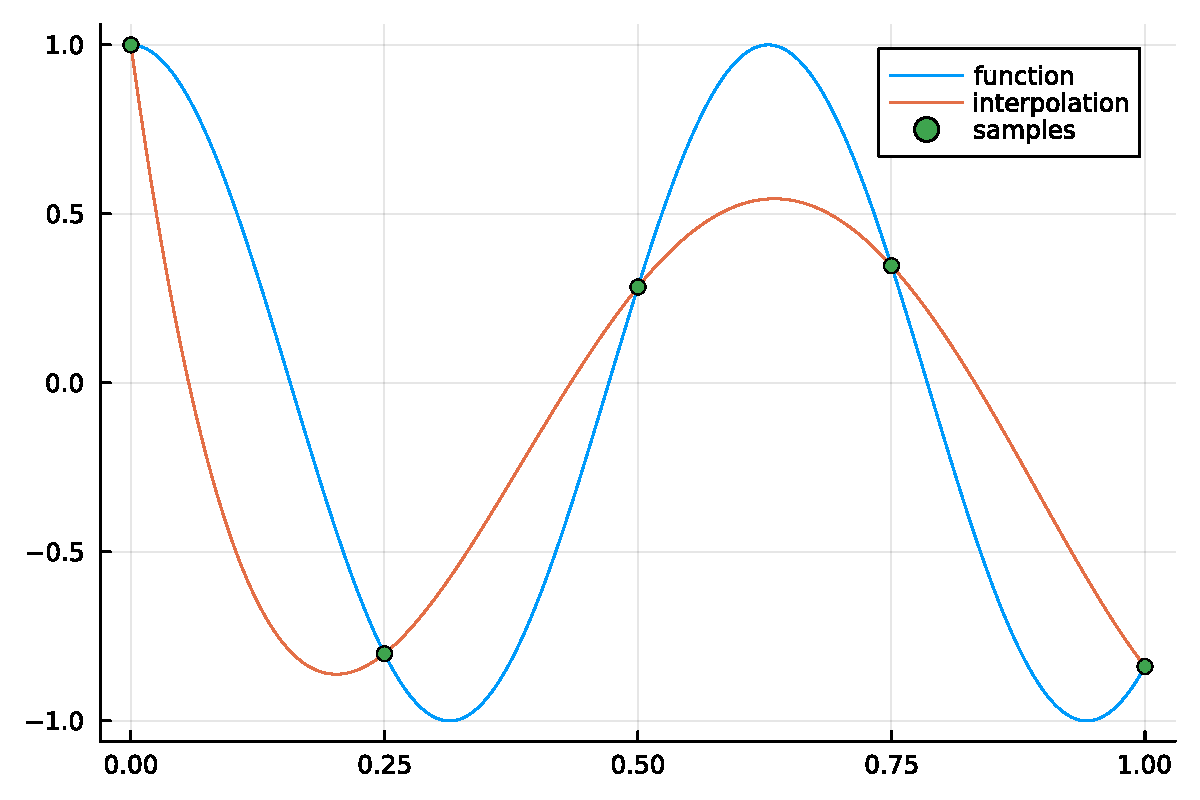
\includegraphics[width=\linewidth]{jl_dOthw0/OP_methods_21_1.pdf}

But it turns out we can also construct the interpolatory polynomial directly. We will use the following with equal $1$ at one grid point and are zero at the others:

\textbf{Definition (Lagrange basis polynomial)} The \emph{Lagrange basis polynomial} is defined as

\[
\ensuremath{\ell}_k(x) := \ensuremath{\prod}_{j \ensuremath{\ne} k} {x-x_j \over x_k - x_j} =  {(x-x_1) \ensuremath{\cdots}(x-x_{k-1})(x-x_{k+1}) \ensuremath{\cdots} (x-x_n) \over (x_k - x_1) \ensuremath{\cdots} (x_k - x_{k-1}) (x_k - x_{k+1}) \ensuremath{\cdots} (x_k - x_n)}
\]
Plugging in the grid points verifies the following:

\textbf{Proposition (delta interpolation)}

\[
\ensuremath{\ell}_k(x_j) = \ensuremath{\delta}_{kj}
\]
We can use these to construct the interpolatory polynomial:

\textbf{Theorem (Lagrange interpolation)} The unique  polynomial of degree at most $n-1$ that interpolates $f$ at $n$ distinct points $x_j$ is:

\[
p(x) = f(x_1) \ensuremath{\ell}_1(x) + \ensuremath{\cdots} + f(x_n) \ensuremath{\ell}_n(x)
\]
\textbf{Proof} Note that

\[
p(x_j) = \ensuremath{\sum}_{j=1}^n f(x_j) \ensuremath{\ell}_k(x_j) = f(x_j)
\]
so we just need to show it is unique. Suppose $p\ensuremath{\tilde}(x)$ is a  polynomial of degree at most $n-1$ that also interpolates $f$. Then $p\ensuremath{\tilde} - p$ vanishes at $n$ distinct points. Thus by the fundamental theorem of algebra it must be zero.

\[
\blacksquare
\]
\textbf{Example} We can interpolate $\exp(x)$ at the points $0,1,2$:


\begin{align*}
p(x) &= \ensuremath{\ell}_1(x) + {\rm e} \ensuremath{\ell}_2(x) + {\rm e}^2 \ensuremath{\ell}_3(x) =
{(x - 1) (x-2) \over (-1)(-2)} + {\rm e} {x (x-2) \over (-1)} +
{\rm e}^2 {x (x-1) \over 2} \\
&= (1/2 - {\rm e} +{\rm e}^2/2)x^2 + (-3/2 + 2 {\rm e}  - {\rm e}^2 /2) x + 1
\end{align*}
\textbf{Remark} Interpolating at evenly spaced points is a really \textbf{bad} idea: interpolation is inheritely ill-conditioned.  The problem sheet asks you to explore this experimentally.

\subsection{2. Roots of orthogonal polynomials and truncated Jacobi matrices}
We now consider roots (zeros) of orthogonal polynomials $p_n(x)$. This is important as we shall see they are useful for interpolation and quadrature. For interpolation to be well-defined we first need to guarantee that the roots are distinct.

\textbf{Lemma} An orthogonal polynomial $p_n(x)$ has exactly $n$ distinct roots.

\textbf{Proof}

Suppose $x_1, \ensuremath{\ldots},x_j$ are the roots where $p_n(x)$ changes sign, that is,

\[
p_n(x) = c_k (x-x_k)^{2p+1} + O((x-x_k)^{2p+2})
\]
for $c_k \ensuremath{\ne} 0$ and $k = 1,\ensuremath{\ldots},j$ and $p \ensuremath{\in} \mathbb{N}$, as $x \ensuremath{\rightarrow} x_k$. Then

\[
p_n(x) (x-x_1) \ensuremath{\cdots}(x-x_j)
\]
does not change signs: it behaves like $c_k (x-x_k)^{2p+2} + O(x-x_k)^{2p+3}$ as $x \ensuremath{\rightarrow} x_k$. In other words:

\[
\ensuremath{\langle}p_n,(x-x_1) \ensuremath{\cdots}(x-x_j) \ensuremath{\rangle} = \int_a^b p_n(x) (x-x_1) \ensuremath{\cdots}(x-x_j) w(x) {\rm d} x \ensuremath{\ne} 0.
\]
where $w(x)$ is the weight of orthogonality. This is only possible if $j = n$ as $p_n(x)$ is orthogonal w.r.t. all lower degree polynomials.

\[
\blacksquare
\]
\textbf{Definition (truncated Jacobi matrix)} Given a symmetric Jacobi matrix $X$, (or the weight $w(x)$ whose orthonormal polynomials are associated with $X$)  the \emph{truncated Jacobi matrix} is

\[
X_n := \begin{bmatrix} a_0 & b_0 \\
                         b_0 & \ensuremath{\ddots} & \ensuremath{\ddots} \\
                         & \ensuremath{\ddots} & a_{n-2} & b_{n-2} \\
                         && b_{n-2} & a_{n-1} \end{bmatrix} \ensuremath{\in} \ensuremath{\bbR}^{n \ensuremath{\times} n}
\]
\textbf{Lemma (zeros)} The zeros $x_1, \ensuremath{\ldots},x_n$ of an orthonormal polynomial $q_n(x)$ are the eigenvalues of the truncated Jacobi matrix $X_n$. More precisely,

\[
X_n Q_n = Q_n \begin{bmatrix} x_1 \\ & \ensuremath{\ddots} \\ && x_n \end{bmatrix}
\]
for the orthogonal matrix

\[
Q_n = \begin{bmatrix}
q_0(x_1) & \ensuremath{\cdots} & q_0(x_n) \\
\ensuremath{\vdots}  & \ensuremath{\cdots} & \ensuremath{\vdots}  \\
q_{n-1}(x_1) & \ensuremath{\cdots} & q_{n-1}(x_n)
\end{bmatrix} \begin{bmatrix} \ensuremath{\alpha}_1^{-1} \\ & \ensuremath{\ddots} \\ && \ensuremath{\alpha}_n^{-1} \end{bmatrix}
\]
where $\ensuremath{\alpha}_j = \sqrt{q_0(x_j)^2 + \ensuremath{\cdots} + q_{n-1}(x_j)^2}$.

\textbf{Proof}

We construct the eigenvector (noting $b_{n-1} q_n(x_j) = 0$):

\[
X_n \begin{bmatrix} q_0(x_j) \\ \ensuremath{\vdots} \\ q_{n-1}(x_j) \end{bmatrix} =
\begin{bmatrix} a_0 q_0(x_j) + b_0 q_1(x_j) \\
 b_0 q_0(x_j) + a_1 q_1(x_j) + b_1 q_2(x_j) \\
\ensuremath{\vdots} \\
b_{n-3} q_{n-3}(x_j) + a_{n-2} q_{n-2}(x_j) + b_{n-2} q_{n-1}(x_j) \\
b_{n-2} q_{n-2}(x_j) + a_{n-1} q_{n-1}(x_j) + b_{n-1} q_n(x_j)
\end{bmatrix} = x_j \begin{bmatrix} q_0(x_j) \\
 q_1(x_j) \\
\ensuremath{\vdots} \\
q_{n-1}(x_j)
\end{bmatrix}
\]
The result follows from normalising the eigenvectors. Since $X_n$ is symmetric the eigenvector matrix is orthogonal. $\blacksquare$

\textbf{Example (Chebyshev roots)} Consider $T_n(x) = \cos n {\rm acos}\, x$. The roots  are $x_j = \cos \ensuremath{\theta}_j$ where $\ensuremath{\theta}_j = (j-1/2)\ensuremath{\pi}/n$ for $j = 1,\ensuremath{\ldots},n$ are the roots of $\cos n \ensuremath{\theta}$ that are inside $[0,\ensuremath{\pi}]$. 

Consider the $n = 3$ case where we have

\[
x_1,x_2,x_3 = \cos(\ensuremath{\pi}/6),\cos(\ensuremath{\pi}/2),\cos(5\ensuremath{\pi}/6) = \sqrt{3}/2,0,-\sqrt{3/2}
\]
We also have from the 3-term recurrence:


\begin{align*}
T_0(x) = 1 \\
T_1(x) = x \\
T_2(x) = 2x T_1(x) - T_0(x) = 2x^2-1 \\
T_3(x) = 2x T_2(x) - T_1(x) = 4x^2-3x
\end{align*}
We orthonormalise by rescaling


\begin{align*}
q_0(x) &= 1/\sqrt{\ensuremath{\pi}} \\
q_k(x) &= T_k(x) \sqrt{2}/\sqrt{\ensuremath{\pi}}
\end{align*}
so that the Jacobi matrix is symmetric:

\[
x [q_0(x)|q_1(x)|\ensuremath{\cdots}] = [q_0(x)|q_1(x)|\ensuremath{\cdots}] \underbrace{\begin{bmatrix} 0 & 1/\sqrt{2} \\
                            1/\sqrt{2} & 0 & 1/2 \\
                            &1/2 & 0 & 1/2 \\
                             &   & 1/2 & 0 & \ensuremath{\ddots} \\
                              &  && \ensuremath{\ddots} & \ensuremath{\ddots}
\end{bmatrix}}_X
\]
We can then confirm that we have constructed an eigenvector/eigenvalue of the $3 \ensuremath{\times} 3$ truncation of the Jacobi matrix, e.g. at $x_2 = 0$:

\[
\begin{bmatrix} 
0 & 1/\sqrt{2} \\
1/\sqrt{2} & 0 & 1/2 \\
    & 1/2 & 0\end{bmatrix} \begin{bmatrix} q_0(0) \\ q_1(0) \\ q_2(0) 
    \end{bmatrix} = {1 \over \sqrt \ensuremath{\pi}} \begin{bmatrix} 
0 & 1/\sqrt{2} \\
1/\sqrt{2} & 0 & 1/2 \\
    & 1/2 & 0\end{bmatrix} \begin{bmatrix} 1 \\ 0 \\ -{1 \over \sqrt{2}}
    \end{bmatrix} =\begin{bmatrix} 0 \\ 0 \\ 0
    \end{bmatrix}
\]
\subsection{3. Interpolatory quadrature rules}
\textbf{Definition (interpolatory quadrature rule)} Given a set of points $\mathbf{x} = [x_1,\ensuremath{\ldots},x_n]$ the interpolatory quadrature rule is:

\[
\ensuremath{\Sigma}_n^{w,\mathbf{x}}[f] := \ensuremath{\sum}_{j=1}^n w_j f(x_j)
\]
where

\[
w_j := \ensuremath{\int}_a^b \ensuremath{\ell}_j(x) w(x) {\rm d} x
\]
\textbf{Proposition (interpolatory quadrature is exact for polynomials)}  Interpolatory quadrature is exact for all degree $n-1$ polynomials $p$:

\[
\ensuremath{\int}_a^b p(x) w(x) {\rm d}x = \ensuremath{\Sigma}_n^{w,\mathbf{x}}[f]
\]
\textbf{Proof} The result follows since, by uniqueness of interpolatory polynomial:

\[
p(x) = \ensuremath{\sum}_{j=1}^n p(x_j) \ensuremath{\ell}_j(x)
\]
\[
\blacksquare
\]
\textbf{Example (arbitrary points)} Find the interpolatory quadrature rule for $w(x) = 1$ on $[0,1]$ with  points $[x_1,x_2,x_3] = [0,1/4,1]$? We have:


\begin{align*}
w_1 = \int_0^1 w(x) \ensuremath{\ell}_1(x) {\rm d}x  = \int_0^1 {(x-1/4)(x-1) \over (-1/4)(-1)}{\rm d}x = -1/6 \\
w_2 = \int_0^1 w(x) \ensuremath{\ell}_2(x) {\rm d}x  = \int_0^1 {x(x-1) \over (1/4)(-3/4)}{\rm d}x = 8/9 \\
w_3 = \int_0^1 w(x) \ensuremath{\ell}_3(x) {\rm d}x  = \int_0^1 {x(x-1/4) \over 3/4}{\rm d}x = 5/18
\end{align*}
That is we have

\[
\ensuremath{\Sigma}_n^{w,\mathbf{x}}[f]  = -{f(0) \over 6} + {8f(1/4) \over 9} + {5 f(1) \over 18}
\]
This is indeed exact for polynomials up to degree $2$ (and no more):

\[
\ensuremath{\Sigma}_n^{w,\mathbf{x}}[1] = 1, \ensuremath{\Sigma}_n^{w,\mathbf{x}}[x] = 1/2, \ensuremath{\Sigma}_n^{w,\mathbf{x}}[x^2] = 1/3, \ensuremath{\Sigma}_n^{w,\mathbf{x}}[x^3] = 7/24 \ensuremath{\ne} 1/4.
\]
\textbf{Example (Chebyshev roots)} Find the interpolatory quadrature rule for $w(x) = 1/\sqrt{1-x^2}$ on $[-1,1]$ with points equal to the roots of $T_3(x)$. This is a special case of Gaussian quadrature which we will approach in another way below. We use:

\[
\int_{-1}^1 w(x) {\rm d}x = \ensuremath{\pi}, \int_{-1}^1 xw(x) {\rm d}x = 0, \int_{-1}^1 x^2 w(x) {\rm d}x = {\ensuremath{\pi}/2}
\]
Recall from before that $x_1,x_2,x_3 = \sqrt{3}/2,0,-\sqrt{3}/2$. Thus we have:


\begin{align*}
w_1 = \int_{-1}^1 w(x) \ensuremath{\ell}_1(x) {\rm d}x = \int_{-1}^1 {x(x+\sqrt{3}/2) \over (\sqrt{3}/2) \sqrt{3} \sqrt{1-x^2}}{\rm d}x = {\ensuremath{\pi} \over 3} \\
w_2 = \int_{-1}^1 w(x) \ensuremath{\ell}_2(x) {\rm d}x = \int_{-1}^1 {(x-\sqrt{3}/2)(x+\sqrt{3}/2) \over (-3/4)\sqrt{1-x^2}}{\rm d}x = {\ensuremath{\pi} \over 3} \\
w_3 = \int_{-1}^1 w(x) \ensuremath{\ell}_3(x) {\rm d}x = \int_{-1}^1 {(x-\sqrt{3}/2) x \over (-\sqrt{3})(-\sqrt{3}/2) \sqrt{1-x^2}}{\rm d}x = {\ensuremath{\pi} \over 3}
\end{align*}
(It's not a coincidence that they are all the same but this will differ for roots of other OPs.)  That is we have

\[
\ensuremath{\Sigma}_n^{w,\mathbf{x}}[f]  = {\ensuremath{\pi} \over 3}(f(\sqrt{3}/2) + f(0) + f(-\sqrt{3}/2)
\]
This is indeed exact for polynomials up to degree $n-1=2$, but it goes all the way up to $2n-1 = 5$:


\begin{align*}
\ensuremath{\Sigma}_n^{w,\mathbf{x}}[1] &= \ensuremath{\pi}, \ensuremath{\Sigma}_n^{w,\mathbf{x}}[x] = 0, \ensuremath{\Sigma}_n^{w,\mathbf{x}}[x^2] = {\ensuremath{\pi} \over 2}, \\
\ensuremath{\Sigma}_n^{w,\mathbf{x}}[x^3] &= 0, \ensuremath{\Sigma}_n^{w,\mathbf{x}}[x^4] &= {3 \ensuremath{\pi} \over 8}, \ensuremath{\Sigma}_n^{w,\mathbf{x}}[x^5] = 0 \\
\ensuremath{\Sigma}_n^{w,\mathbf{x}}[x^6] &= {9 \ensuremath{\pi} \over 32} \ensuremath{\ne} {5 \ensuremath{\pi} \over 16}
\end{align*}
We shall explain this miracle next.

\subsection{4. Gaussian quadrature}
Gaussian quadrature is the interpolatory quadrature rule corresponding to the grid $x_j$ defined as the roots of the orthonormal polynomial $q_n(x)$. We shall see that it is exact for polynomials up to degree $2n-1$, i.e., double the degree of other interpolatory quadrature rules from other grids.

\textbf{Definition (Gauss quadrature)} Given a weight $w(x)$, the Gauss quadrature rule is:

\[
\ensuremath{\int}_a^b f(x)w(x) {\rm d}x \ensuremath{\approx} \underbrace{\ensuremath{\sum}_{j=1}^n w_j f(x_j)}_{\ensuremath{\Sigma}_n^w[f]}
\]
where $x_1,\ensuremath{\ldots},x_n$ are the roots of the orthonormal polynomials $q_n(x)$ and 

\[
w_j := {1 \over \ensuremath{\alpha}_j^2} = {1 \over q_0(x_j)^2 + \ensuremath{\cdots} + q_{n-1}(x_j)^2}.
\]
Equivalentally, $x_1,\ensuremath{\ldots},x_n$ are the eigenvalues of $X_n$ and

\[
w_j = \ensuremath{\int}_a^b w(x) {\rm d}x Q_n[1,j]^2.
\]
(Note we have $\ensuremath{\int}_a^b w(x) {\rm d} x q_0(x)^2 = 1$.)

In analogy to how Fourier series are orthogonal with respect to Trapezium rule, Orthogonal polynomials are orthogonal with respect to Gaussian quadrature:

\textbf{Lemma (Discrete orthogonality)} For $0 \ensuremath{\leq} \ensuremath{\ell},m \ensuremath{\leq} n-1$, the orthonormal polynomials $q_n(x)$ satisfy

\[
\ensuremath{\Sigma}_n^w[q_\ensuremath{\ell} q_m] = \ensuremath{\delta}_{\ensuremath{\ell}m}
\]
\textbf{Proof}

\[
\ensuremath{\Sigma}_n^w[q_\ensuremath{\ell} q_m] = \ensuremath{\sum}_{j=1}^n {q_\ensuremath{\ell}(x_j) q_m(x_j) \over \ensuremath{\alpha}_j^2}
= \left[q_\ensuremath{\ell}(x_1)/ \ensuremath{\alpha}_1 | \ensuremath{\cdots} | {q_\ensuremath{\ell}(x_n)/ \ensuremath{\alpha}_n}\right] 
\begin{bmatrix}
q_m(x_1)/\ensuremath{\alpha}_1 \\
\ensuremath{\vdots} \\
q_m(x_n)/\ensuremath{\alpha}_n \end{bmatrix} = \mathbf{e}_\ensuremath{\ell} Q_n Q_n^\ensuremath{\top} \mathbf{e}_m = \ensuremath{\delta}_{\ensuremath{\ell}m}
\]
\[
\blacksquare
\]
Just as approximating Fourier coefficients using Trapezium rule gives a way of interpolating at the grid, so does Gaussian quadrature:

\textbf{Theorem (interpolation via quadrature)} For the orthonormal polynomials $q_n(x)$,

\[
f_n(x) = \ensuremath{\sum}_{k=0}^{n-1} c_k^n q_k(x)\hbox{ for } c_k^n := \ensuremath{\Sigma}_n^w[f q_k]
\]
interpolates $f(x)$ at the Gaussian quadrature points $x_1,\ensuremath{\ldots},x_n$.

\textbf{Proof}

Consider the Vandermonde-like matrix:

\[
\tilde{V} := \begin{bmatrix} q_0(x_1) & \ensuremath{\cdots} & q_{n-1}(x_1) \\
                \ensuremath{\vdots} & \ensuremath{\ddots} & \ensuremath{\vdots} \\
                q_0(x_n) & \ensuremath{\cdots} & q_{n-1}(x_n) \end{bmatrix}
\]
and define

\[
Q_n^w := \tilde{V}^{\top} \begin{bmatrix} w_1 \\ &\ensuremath{\ddots} \\&& w_n \end{bmatrix} = \begin{bmatrix} q_0(x_1)w_1 & \ensuremath{\cdots} &  q_0(x_n) w_n \\
                \ensuremath{\vdots} & \ensuremath{\ddots} & \ensuremath{\vdots} \\
                w_1q_{n-1}(x_1) & \ensuremath{\cdots} & q_{n-1}(x_n)w_n \end{bmatrix}
\]
so that

\[
\begin{bmatrix}
c_0^n \\
\ensuremath{\vdots} \\
c_{n-1}^n \end{bmatrix} = Q_n^w \begin{bmatrix} f(x_1) \\ \ensuremath{\vdots} \\ f(x_n) \end{bmatrix}.
\]
Note that if $p(x) = [q_0(x) | \ensuremath{\cdots} | q_{n-1}(x)] \mathbf{c}$ then

\[
\begin{bmatrix}
p(x_1) \\
\ensuremath{\vdots} \\
p(x_n)
\end{bmatrix} = \tilde{V} \mathbf{c}
\]
But we see that (similar to the Fourier case)

\[
Q_n^w \tilde{V} = \begin{bmatrix} \ensuremath{\Sigma}_n^w[q_0 q_0] & \ensuremath{\cdots} & \ensuremath{\Sigma}_n^w[q_0 q_{n-1}]\\
                \ensuremath{\vdots} & \ensuremath{\ddots} & \ensuremath{\vdots} \\
                \ensuremath{\Sigma}_n^w[q_{n-1} q_0] & \ensuremath{\cdots} & \ensuremath{\Sigma}_n^w[q_{n-1} q_{n-1}]
                \end{bmatrix} = I_n
\]
\[
\blacksquare
\]
\textbf{Corollary} Gaussian quadrature is an interpolatory quadrature rule with the interpolation points equal to the roots of $q_n$:

\[
\ensuremath{\Sigma}_n^w[f] = \ensuremath{\Sigma}_n^{w,\mathbf{x}}[f]
\]
\textbf{Proof} We want to show its the same as integrating the interpolatory polynomial:

\[
\int_a^b f_n(x) w(x) {\rm d}x = {1 \over q_0(x)} \sum_{k=0}^{n-1} c_k^n \int_a^b q_k(x) q_0(x) w(x) {\rm d}x
= {c_0^n \over q_0} = \ensuremath{\Sigma}_n^w[f].
\]
\[
\blacksquare
\]
A consequence of being an interpolatory quadrature rule is that it is exact for all polynomials of degree $n-1$. The \emph{miracle} of Gaussian quadrature is it is exact for twice as many!

\textbf{Theorem (Exactness of Gauss quadrature)} If $p(x)$ is a degree $2n-1$ polynomial then Gauss quadrature is exact:

\[
\ensuremath{\int}_a^b p(x)w(x) {\rm d}x = \ensuremath{\Sigma}_n^w[p].
\]
\textbf{Proof} Using polynomial division algorithm (e.g. by matching terms) we can write

\[
p(x) = q_n(x) s(x) + r(x)
\]
where $s$ and $r$ are degree $n-1$ and $q_n(x)$ is the degree $n$ orthonormal polynomial. Then we have:


\begin{align*}
\ensuremath{\Sigma}_n^w[p] &= \underbrace{\ensuremath{\Sigma}_n^w[q_n s]}_{\hbox{$0$ since evaluating $q_n$ at zeros}} + \ensuremath{\Sigma}_n^w[r] = \ensuremath{\int}_a^b r(x) w(x) {\rm d}x
= \underbrace{\ensuremath{\int}_a^b q_n(x)s(x) w(x) {\rm d}x}_{\hbox{$0$ since $s$ is degree $<n$}}  + \ensuremath{\int}_a^b r(x) w(x) {\rm d}x \\
&= \ensuremath{\int}_a^b p(x)w(x) {\rm d}x.
\end{align*}
\[
\blacksquare
\]
\textbf{Example (Chebyshev expansions)}  Consider the construction of Gaussian quadrature for $n = 3$. To determine the weights we need:

\[
w_j^{-1} = \ensuremath{\alpha}_j^2 = q_0(x_j)^2 + q_1(x_j)^2 + q_2(x_j)^2 = 
{1 \over \ensuremath{\pi}} + {2 \over \ensuremath{\pi}} x_j^2 + {2 \over \ensuremath{\pi}} (2x_j^2-1)^2
\]
We can check each case and deduce that $w_j = \ensuremath{\pi}/3$. Thus we recover the interpolatory quadrature rule. Further, we can construct the transform


\begin{align*}
Q_3^w &= \begin{bmatrix}
w_1 q_0(x_1) & w_2 q_0(x_2) & w_3 q_0(x_3) \\
w_1 q_1(x_1) & w_2 q_1(x_2) & w_3 q_1(x_3) \\
w_1 q_3(x_1) & w_2 q_3(x_2) & w_3 q_3(x_3) 
\end{bmatrix}\\
&= {\ensuremath{\pi} \over 3} \begin{bmatrix} 1/\sqrt{\ensuremath{\pi}} & 1/\sqrt{\ensuremath{\pi}} & 1/\sqrt{\ensuremath{\pi}} \\
                                x_1\sqrt{2/\ensuremath{\pi}} & x_2\sqrt{2/\ensuremath{\pi}} & x_3\sqrt{2/\ensuremath{\pi}} \\
                                (2x_1^2-1)\sqrt{2/\ensuremath{\pi}} &(2x_2^2-1)\sqrt{2/\ensuremath{\pi}} & (2x_3^2-1)\sqrt{2/\ensuremath{\pi}}
                                \end{bmatrix} \\
                                &= 
                                {\sqrt{\ensuremath{\pi}} \over 3} \begin{bmatrix} 1 & 1 & 1 \\
                                \sqrt{6}/2 & 0 & -\sqrt{6}/2 \\
                                1/\sqrt{2} &-\sqrt{2} & 1/\sqrt{2}
                                \end{bmatrix}
\end{align*}
We can use this to expand a polynomial, e.g. $x^2$:

\[
Q_3^2 \begin{bmatrix}
x_1^2 \\
x_2^2 \\
x_3^2 
\end{bmatrix} = {\sqrt{\ensuremath{\pi}} \over 3} 
\begin{bmatrix} 1 & 1 & 1 \\
\sqrt{6}/2 & 0 & -\sqrt{6}/2 \\
1/\sqrt{2} &-\sqrt{2} & 1/\sqrt{2}
\end{bmatrix} 
\begin{bmatrix} 3/4 \\ 0 \\ 3/4 \end{bmatrix} =
\begin{bmatrix}
{\sqrt{\ensuremath{\pi}} / 2} \\
0 \\
{\sqrt{\ensuremath{\pi}} / (2\sqrt{2})}
\end{bmatrix}
\]
In other words:

\[
x^2 = {\sqrt \ensuremath{\pi} \over 2} q_0(x) + {\sqrt \ensuremath{\pi} \over 2\sqrt 2} q_2(x) = {1 \over 2} T_0(x) + {1 \over 2} T_2(x)
\]
which can be easily confirmed.

\subsection{Approximation with Chebyshev polynomials}
Previously, we used the formula, derived via trigonometric manipulations,

\[
T_1(x) = x T_0(x), \qquad
T_{n+1}(x) = 2x T_n(x) - T_{n-1}(x)
\]
Rearranging, this becomes

\[
 x T_0(x) = T_1(x), \qquad
x T_n(x)  =  {T_{n-1}(x) \over 2} + {T_{n+1}(x) \over 2}
\]
This tells us that we have the three-term recurrence with $a_n = 0$, $b_0 = 1$, $c_n = b_n = {1 \over 2}$ for $n > 0$.

This can be extended to function approximation. Provided the sum converges absolutely and uniformly in $x$, we can write

\[
f(x) = \sum_{k=0}^\infty f_k T_k(x).
\]
In practice, we can approximate smooth functions by a finite truncation:

\[
f(x) \approx \sum_{k=0}^{n-1} f_k T_k(x)
\]
Here we see that ${\rm e}^x$ can be approximated by a Chebyshev approximation using 14 coefficients and is accurate to 16 digits:


\begin{lstlisting}
(*@\HLJLn{f}@*) (*@\HLJLoB{=}@*) (*@\HLJLnf{Fun}@*)(*@\HLJLp{(}@*)(*@\HLJLn{x}@*) (*@\HLJLoB{->}@*) (*@\HLJLnf{exp}@*)(*@\HLJLp{(}@*)(*@\HLJLn{x}@*)(*@\HLJLp{),}@*) (*@\HLJLnf{Chebyshev}@*)(*@\HLJLp{())}@*)
(*@\HLJLnf{scatter}@*)(*@\HLJLp{(}@*)(*@\HLJLni{0}@*)(*@\HLJLoB{:}@*)(*@\HLJLnf{ncoefficients}@*)(*@\HLJLp{(}@*)(*@\HLJLn{f}@*)(*@\HLJLp{)}@*)(*@\HLJLoB{-}@*)(*@\HLJLni{1}@*)(*@\HLJLp{,}@*)(*@\HLJLn{abs}@*)(*@\HLJLoB{.}@*)(*@\HLJLp{(}@*)(*@\HLJLn{f}@*)(*@\HLJLoB{.}@*)(*@\HLJLn{coefficients}@*)(*@\HLJLp{);}@*)(*@\HLJLn{yscale}@*)(*@\HLJLoB{=:}@*)(*@\HLJLn{log10}@*)(*@\HLJLp{,}@*)(*@\HLJLn{label}@*)(*@\HLJLoB{=}@*)(*@\HLJLs{"{}Chebyshev}@*) (*@\HLJLs{coefficients,}@*) (*@\HLJLs{f\ensuremath{\_k}"{}}@*)(*@\HLJLp{,}@*)(*@\HLJLn{xlabel}@*)(*@\HLJLoB{=}@*)(*@\HLJLs{"{}k"{}}@*)(*@\HLJLp{)}@*)
\end{lstlisting}

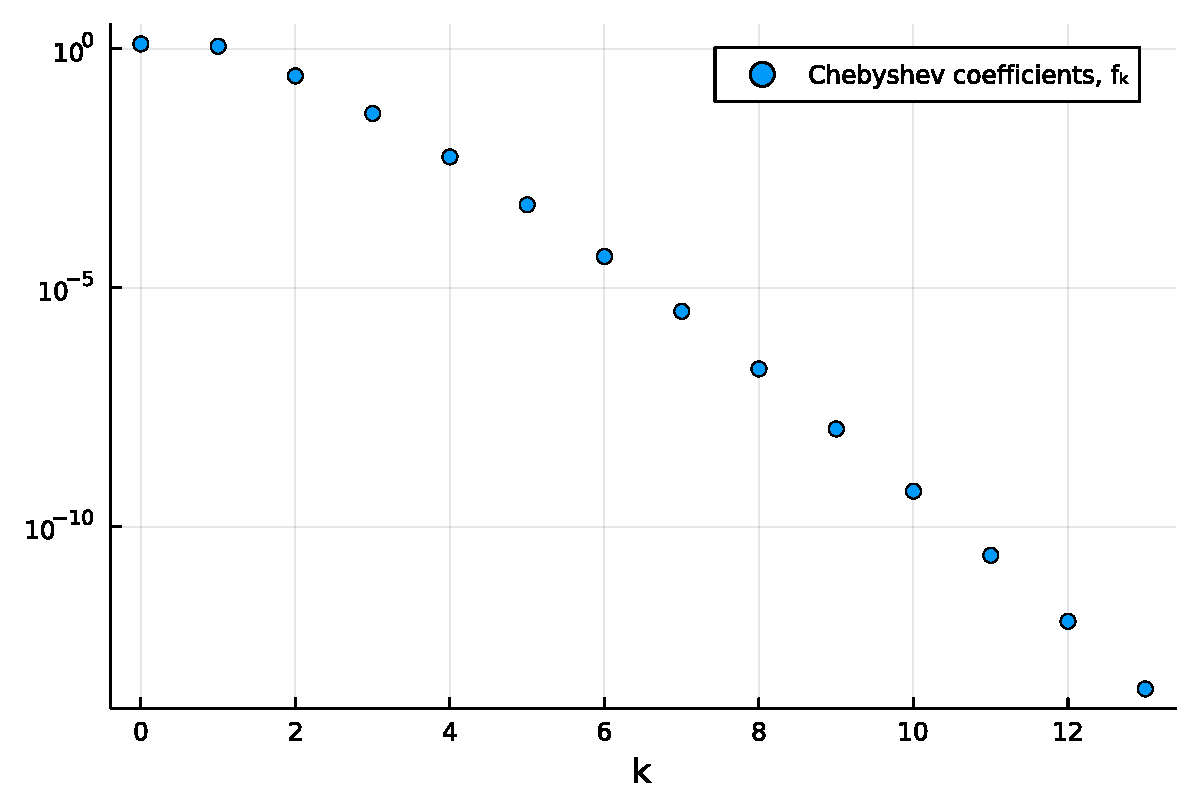
\includegraphics[width=\linewidth]{jl_dOthw0/OP_methods_22_1.pdf}

\begin{lstlisting}
(*@\HLJLnd{@show}@*) (*@\HLJLnf{ncoefficients}@*)(*@\HLJLp{(}@*)(*@\HLJLn{f}@*)(*@\HLJLp{)}@*)
(*@\HLJLnd{@show}@*) (*@\HLJLnf{f}@*)(*@\HLJLp{(}@*)(*@\HLJLnfB{0.1}@*)(*@\HLJLp{)}@*) (*@\HLJLcs{{\#}}@*) (*@\HLJLcs{equivalent}@*) (*@\HLJLcs{to}@*) (*@\HLJLcs{f.coefficients{\textquotesingle}*[cos(k*acos(x))}@*) (*@\HLJLcs{for}@*) (*@\HLJLcs{k=0:ncoefficients(f)-1]}@*)
(*@\HLJLnd{@show}@*) (*@\HLJLnf{exp}@*)(*@\HLJLp{(}@*)(*@\HLJLnfB{0.1}@*)(*@\HLJLp{);}@*)
\end{lstlisting}

\begin{lstlisting}
ncoefficients(f) = 14
f(0.1) = 1.1051709180756477
exp(0.1) = 1.1051709180756477
\end{lstlisting}


The accuracy of this approximation is typically dictated by the smoothness of $f$: the more times we can differentiate, the faster it converges. For analytic functions, it's dictated by the domain of analyticity, just like Laurent/Fourier series. In the case above, ${\rm e}^x$ is entire hence we get faster than exponential convergence.

Chebyshev expansions work even when Taylor series do not. For example, the following function has poles at $\pm {{\rm i} \over 5}$, which means the radius of convergence for the Taylor series is $|x| < {1 \over 5}$, but Chebyshev polynomials continue to work on $[-1,1]$:


\begin{lstlisting}
(*@\HLJLn{f}@*) (*@\HLJLoB{=}@*) (*@\HLJLnf{Fun}@*)(*@\HLJLp{(}@*) (*@\HLJLn{x}@*) (*@\HLJLoB{->}@*) (*@\HLJLni{1}@*)(*@\HLJLoB{/}@*)(*@\HLJLp{(}@*)(*@\HLJLni{25}@*)(*@\HLJLn{x}@*)(*@\HLJLoB{{\textasciicircum}}@*)(*@\HLJLni{2}@*) (*@\HLJLoB{+}@*) (*@\HLJLni{1}@*)(*@\HLJLp{),}@*) (*@\HLJLnf{Chebyshev}@*)(*@\HLJLp{())}@*)
(*@\HLJLnd{@show}@*) (*@\HLJLnf{ncoefficients}@*)(*@\HLJLp{(}@*)(*@\HLJLn{f}@*)(*@\HLJLp{)}@*)
(*@\HLJLnf{plot}@*)(*@\HLJLp{(}@*)(*@\HLJLn{f}@*)(*@\HLJLp{;}@*)(*@\HLJLn{label}@*)(*@\HLJLoB{=}@*)(*@\HLJLkc{false}@*)(*@\HLJLp{)}@*)
\end{lstlisting}

\begin{lstlisting}
ncoefficients(f) = 189
\end{lstlisting}

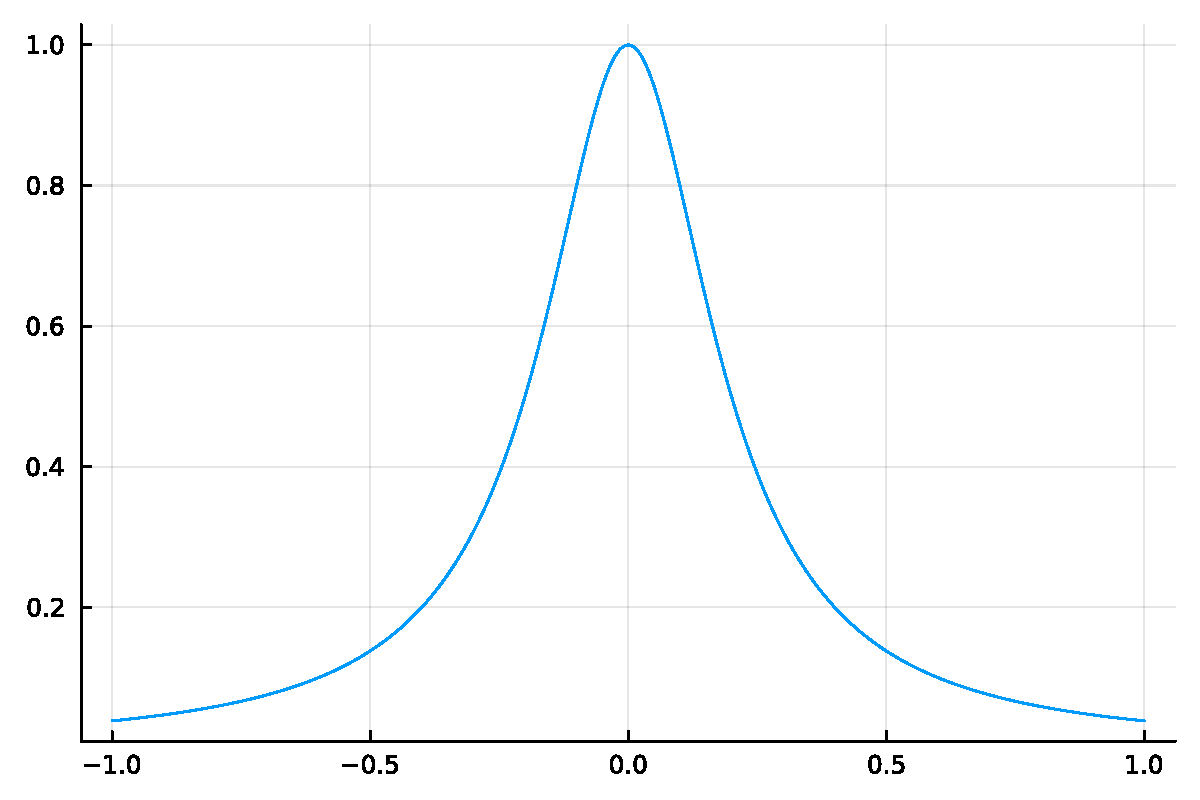
\includegraphics[width=\linewidth]{jl_dOthw0/OP_methods_24_1.pdf}

This can be explained for Chebyshev expansion by noting that it is the cosine expansion / Fourier expansion of an even function:

\[
f(x) = \sum_{k=0}^\infty f_k T_k(x) \Leftrightarrow f(\cos \theta) = \sum_{k=0}^\infty f_k \cos k \theta
\]
\subsubsection{Exponential decay of Fourier coefficients of periodic, analytic functions revisited}
Before we get to the decay of Chebyshev coefficients, we revisit the proof of the exponential decay of \emph{Fourier} coefficients in Lecture 6. Suppose $f(\theta)$ is $2\pi$-periodic and analytic on $\theta \in [-\pi, \pi)$, then

\[
    f(\theta) = \sum_{k=-\infty}^\infty \hat f_k {\rm e}^{{\rm i} k \theta}
\]
where

\[
\hat f_k = {1\over 2 \pi} \int_{-\pi}^\pi f(\theta){\rm e}^{-{\rm i} k \theta} {\rm d} \theta.
\]
Recall in Lecture 6 we set $z = {\rm e}^{{\rm i} \theta}$ in which case the Fourier series of $f$ becomes a Laurent series of a function $g(z)$:

\[
f(\theta) = \sum_{k=-\infty}^\infty \hat f_k {\rm e}^{{\rm i} k \theta} = \sum_{k=-\infty}^\infty g_k z^k =: g(z),
\]
with $g_k = \hat f_k$. We proved that if $g(z)$ is analytic on the closed annulus $A_{r,R} = \lbrace z : r \leq \vert z \vert \leq R \rbrace$, $0 < r <1$, $R > 1$ then for all $k \in \mathbb{Z}$, $|g_k | \leq M\min\left\{{1 \over R^k} , {1 \over r^k}\right\}$ where $M = \sup_{z \in  A_{r,R}} |g(z)|$. This result implies the exponential decay of the Fourier coefficients of $f$.

An annulus in the $z$-plane corresponds to a strip of width $2\pi$ in the (complex) $\theta$-plane under the transformation $z = {\rm e}^{{\rm i} \theta}$, $\Re \theta \in [-\pi, \pi)$:


\begin{align*}
& z \in A_{r,R} = \lbrace z : r \leq \vert z \vert \leq R \rbrace \qquad \underbrace{\Longleftrightarrow}_{z = {\rm e}^{{\rm i} \theta}} \\
& \theta \in  S_{r,R} =   \lbrace \theta : -\pi \leq \Re  \theta < \pi,  -\log(R) \leq \Im \theta \leq \log(1/r) \rbrace.
\end{align*}
Suppose $f(\theta)$ is real-valued on $[-\pi, \pi)$, then $\overline{f(\theta)} = f(\overline{\theta})$. Hence if the closest singularity to the real $\theta$-axis is at $\theta = \theta_x + {\rm i} \theta_y$, with $\theta_x \in [-\pi, \pi)$ and $\theta_y > 0$, then $f$ also has a singularity at  $\theta_x - {\rm i} \theta_y$. Thus $f$ is analytic in the strip

\[
S_{r,R} = \theta \in    \lbrace \theta : -\pi \leq \Re  \theta < \pi,  -\log(R) \leq \Im \theta \leq \log(1/r) \rbrace
\]
with

\[
{1 \over r} = R < {\rm e}^{\theta_y}
\]
and the Fourier coefficients are bounded by

\[
|f_k | = |g_k |  \leq M\min\left\{{1 \over R^k} , {1 \over r^k}\right\} = M r^{|k|} = M R^{-|k|}, \qquad k \in \mathbb{Z},
\]
where $M = \sup_{z \in  A_{r,R}} |g(z)| = \sup_{\theta \in  S_{r,R}} |f(\theta)|$. The larger the strip of analyticity, the larger we can make $R$ and the faster the Fourier coefficients of $f$ decay as $\vert k \vert \to \infty$ (hence the faster the truncated Fourier expansion $\sum_{k=-n}^{n}\hat f_k {\rm e}^{{\rm i} k \theta}$ of $f$ converges to $f$ as $n \to \infty$).

\emph{Example (see also Lecture 6)} The function

\[
 f(\theta) = {1 \over 2 - \cos\theta},
\]
has poles at $\theta = \pm {\rm i} \log (2 + \sqrt{3})$; it is analytic in the strip $S_{r,R}$ with $R = 1/r < 2 + \sqrt{3}$ and the maximum of $\vert f(\theta) \vert$ on $S_{r,R}$ is

\[
M = {2 \over 4 - R^{-1} + R},
\]
hence

\[
|f_k| =     |g_k| \leq {2 \over 4 - R -R^{-1}} R^{-\vert k \vert}, \qquad k \in \mathbb{Z},
\]
for all $R < 2 + \sqrt{3}$.


\begin{lstlisting}
(*@\HLJLcs{{\#}}@*) (*@\HLJLcs{This}@*) (*@\HLJLcs{works}@*) (*@\HLJLcs{in}@*) (*@\HLJLcs{Julia}@*) (*@\HLJLcs{1.7.2,}@*) (*@\HLJLcs{just}@*) (*@\HLJLcs{use}@*) (*@\HLJLcs{the}@*) (*@\HLJLcs{FFT}@*)
(*@\HLJLcs{{\#}g}@*) (*@\HLJLcs{=Fun(\ensuremath{\theta}}@*) (*@\HLJLcs{->}@*) (*@\HLJLcs{1/(2-cos(\ensuremath{\theta})),}@*) (*@\HLJLcs{Laurent(-\ensuremath{\pi}}@*) (*@\HLJLcs{..}@*) (*@\HLJLcs{\ensuremath{\pi}))}@*)
(*@\HLJLcs{{\#}g\ensuremath{\_+}}@*) (*@\HLJLcs{=}@*) (*@\HLJLcs{g.coefficients[1:2:end]}@*)
(*@\HLJLcs{{\#}scatter(abs.(g\ensuremath{\_+});}@*) (*@\HLJLcs{yscale=:log10,}@*) (*@\HLJLcs{label="{}|g{\_}k|"{},}@*) (*@\HLJLcs{legend=:bottomleft,xlabel="{}k"{})}@*)
(*@\HLJLcs{{\#}R}@*) (*@\HLJLcs{=}@*) (*@\HLJLcs{1.1}@*)
(*@\HLJLcs{{\#}scatter!(2/(4-R-inv(R))*R.{\textasciicircum}(-(0:length(g\ensuremath{\_+}))),}@*) (*@\HLJLcs{label}@*) (*@\HLJLcs{=}@*) (*@\HLJLcs{"{}R}@*) (*@\HLJLcs{=}@*) (*@\HLJLcs{{\$}R"{})}@*)
(*@\HLJLcs{{\#}R}@*) (*@\HLJLcs{=}@*) (*@\HLJLcs{3.5}@*)
(*@\HLJLcs{{\#}scatter!(2/(4-R-inv(R))*R.{\textasciicircum}(-(0:length(g\ensuremath{\_+}))),}@*) (*@\HLJLcs{label}@*) (*@\HLJLcs{=}@*) (*@\HLJLcs{"{}R}@*) (*@\HLJLcs{=}@*) (*@\HLJLcs{{\$}R"{})}@*)
(*@\HLJLcs{{\#}R}@*) (*@\HLJLcs{=}@*) (*@\HLJLcs{2+sqrt(3)-0.1}@*)
(*@\HLJLcs{{\#}scatter!(2/(4-R-inv(R))*R.{\textasciicircum}(-(0:length(g\ensuremath{\_+}))),}@*) (*@\HLJLcs{label}@*) (*@\HLJLcs{=}@*) (*@\HLJLcs{"{}R}@*) (*@\HLJLcs{=}@*) (*@\HLJLcs{{\$}R"{})}@*)
\end{lstlisting}


\subsubsection{Exponential decay of Chebyshev coefficients of analytic functions}
Suppose $f(x)$ is analytic on $[-1, 1]$, then


\begin{align*}
f(x) & = \sum_{k = 0}^{\infty} f_k T_k(x) \\
     & =\sum_{k = 0}^{\infty} f_k \cos k\theta \qquad (x = \cos\theta) \\
     & = \sum_{k = 0}^{\infty} {f_k \over 2}\left( z^k + z^{-k}\right)  \qquad (z = {\rm e}^{{\rm i} \theta}) \\
     & =: \sum_{k = -\infty}^{\infty} g_k z^{k} =: g(z) \qquad (g_0 = f_0, g_{k} = g_{-k} = f_k/2, k\geq 0)
\end{align*}
Now we can use the bound on the Laurent coefficients of $g(z)$ to bound the Chebyshev coefficients of $f(x)$. First we need to establish what is the image in the (complex) $x$-plane of an annulus in the $z$-plane under the transformation $2x = z + z^{-1}$, which is known as the Joukowsky map.

Let $\rho > 1$ and

\[
A_{1,\rho} =  \lbrace z : 1 \leq \vert z \vert \leq \rho \rbrace, \qquad  A_{\rho^{-1},1} =  \lbrace z : \rho^{-1} \leq \vert z \vert \leq 1 \rbrace.
\]
The Joukowsky transformation maps $A_{1,\rho}$ and $A_{\rho^{-1},1}$ to the following ellipse (known as a Bernstein ellipse) in the $x$-plane:

\[
E_{\rho} = \left\lbrace x : {(\Re x)^2 \over \alpha^2} + {({\rm i}m x)^2 \over \beta^2} \leq 1, \alpha = {1 \over 2}\left( \rho + \rho^{-1} \right),   \beta = {1 \over 2}\left( \rho - \rho^{-1} \right) \right\rbrace.
\]
We conclude that if $f(x)$ is analytic on $E_{\rho}$ (or $g(z)$ is analytic on $A_{\rho^{-1},\rho}$) and $M = \sup_{x \in  E_{\rho}} |f(x)| = \sup_{z \in  A_{\rho^{-1},\rho}} |g(z)|$, then

\[
\vert f_k \vert = 2 \vert g_k \vert \leq 2M\rho^{-k}, \qquad k \geq 1.
\]
The larger the Bernstein ellipse on which $f(x)$ is analytic, the faster the decay of the Chebyshev coefficients as $k \to \infty$ (and hence the faster the convergence of the Chebyshev expansion of $f$).

A truncated Chebyshev expansion with $n$ terms of a function $f(x)$ that is analytic on $E_{\rho}$ converges at essentially the same exponential rate as the bound on the Chebyshev coefficients as $n \to \infty$:


\begin{align*}
\left \vert f(x) -   \sum_{k = 0}^{n-1}f_kT_k(x) \right\vert & = \left \vert  \sum_{k = n}^{\infty}f_kT_k(x) \right\vert \leq \sum_{k = n}^{\infty}\vert f_k \vert \leq 2M \sum_{k = n}^{\infty} \rho^{-k}\\
& = 2M \frac{\rho^{-n}}{1 - \rho^{-1}}
\end{align*}
\emph{Example}  In the case of $f(x) = {1 \over 25 x^2 + 1}$, setting $2x = z + z^{-1}$, we find that

\[
f(x) = f\left( {z+z^{-1} \over 2 } \right) = g(z) = {4 z^2 \over 25 + 54 z^2 + 25 z^4}.
\]
In the complex $x$-plane, $f(x)$ has poles at $\pm {\rm i}/5$ and is analytic on $E_{\rho}$ with $\beta = (\rho - \rho^{-1})/2 < 1/5$, hence $\rho < { 1 + \sqrt{26} \over 5 }$. In the $z$-plane, $g(z)$ has poles at $\pm {\rm i} { 1 \pm \sqrt{26} \over 5 } \approx \pm 0.8198040{\rm i},\pm1.2198{\rm i}$ and is analytic on the annulus $\rho^{-1} \leq \vert z \vert \leq \rho$.


\begin{lstlisting}
(*@\HLJLn{\ensuremath{\rho}}@*) (*@\HLJLoB{=}@*) (*@\HLJLp{(}@*)(*@\HLJLni{1}@*) (*@\HLJLoB{+}@*) (*@\HLJLnf{sqrt}@*)(*@\HLJLp{(}@*)(*@\HLJLni{26}@*)(*@\HLJLp{))}@*)(*@\HLJLoB{/}@*)(*@\HLJLni{5}@*)(*@\HLJLoB{-}@*)(*@\HLJLnfB{0.05}@*)(*@\HLJLp{;}@*)
(*@\HLJLn{\ensuremath{\alpha}}@*) (*@\HLJLoB{=}@*) (*@\HLJLp{(}@*)(*@\HLJLn{\ensuremath{\rho}}@*) (*@\HLJLoB{+}@*) (*@\HLJLni{1}@*)(*@\HLJLoB{/}@*)(*@\HLJLn{\ensuremath{\rho}}@*)(*@\HLJLp{)}@*)(*@\HLJLoB{/}@*)(*@\HLJLni{2}@*)
(*@\HLJLn{\ensuremath{\beta}}@*) (*@\HLJLoB{=}@*) (*@\HLJLp{(}@*)(*@\HLJLn{\ensuremath{\rho}}@*) (*@\HLJLoB{-}@*) (*@\HLJLni{1}@*)(*@\HLJLoB{/}@*)(*@\HLJLn{\ensuremath{\rho}}@*)(*@\HLJLp{)}@*)(*@\HLJLoB{/}@*)(*@\HLJLni{2}@*)
(*@\HLJLn{\ensuremath{\theta}}@*) (*@\HLJLoB{=}@*) (*@\HLJLoB{-}@*)(*@\HLJLn{\ensuremath{\pi}}@*)(*@\HLJLoB{:}@*)(*@\HLJLnfB{0.01}@*)(*@\HLJLoB{:}@*)(*@\HLJLn{\ensuremath{\pi}}@*)
(*@\HLJLn{f}@*) (*@\HLJLoB{=}@*) (*@\HLJLn{x}@*) (*@\HLJLoB{->}@*) (*@\HLJLni{1}@*)(*@\HLJLoB{/}@*)(*@\HLJLp{(}@*)(*@\HLJLni{25}@*)(*@\HLJLn{x}@*)(*@\HLJLoB{{\textasciicircum}}@*)(*@\HLJLni{2}@*) (*@\HLJLoB{+}@*) (*@\HLJLni{1}@*)(*@\HLJLp{)}@*)
(*@\HLJLnf{phaseplot}@*)(*@\HLJLp{(}@*)(*@\HLJLoB{-}@*)(*@\HLJLnfB{2..2}@*)(*@\HLJLp{,}@*) (*@\HLJLoB{-}@*)(*@\HLJLnfB{2..2}@*)(*@\HLJLp{,}@*) (*@\HLJLn{z}@*) (*@\HLJLoB{->}@*) (*@\HLJLnf{f}@*)(*@\HLJLp{(}@*)(*@\HLJLn{z}@*)(*@\HLJLp{))}@*)
(*@\HLJLnf{plot!}@*)(*@\HLJLp{(}@*)(*@\HLJLn{\ensuremath{\alpha}}@*)(*@\HLJLoB{*}@*)(*@\HLJLn{cos}@*)(*@\HLJLoB{.}@*)(*@\HLJLp{(}@*)(*@\HLJLn{\ensuremath{\theta}}@*)(*@\HLJLp{),}@*)(*@\HLJLn{\ensuremath{\beta}}@*)(*@\HLJLoB{*}@*)(*@\HLJLn{sin}@*)(*@\HLJLoB{.}@*)(*@\HLJLp{(}@*)(*@\HLJLn{\ensuremath{\theta}}@*)(*@\HLJLp{);}@*)(*@\HLJLn{linecolor}@*)(*@\HLJLoB{=}@*)(*@\HLJLs{"{}black"{}}@*)(*@\HLJLp{,}@*)(*@\HLJLn{label}@*)(*@\HLJLoB{=}@*)(*@\HLJLs{"{}Bernstein}@*) (*@\HLJLs{ellipse"{}}@*)(*@\HLJLp{)}@*)
\end{lstlisting}

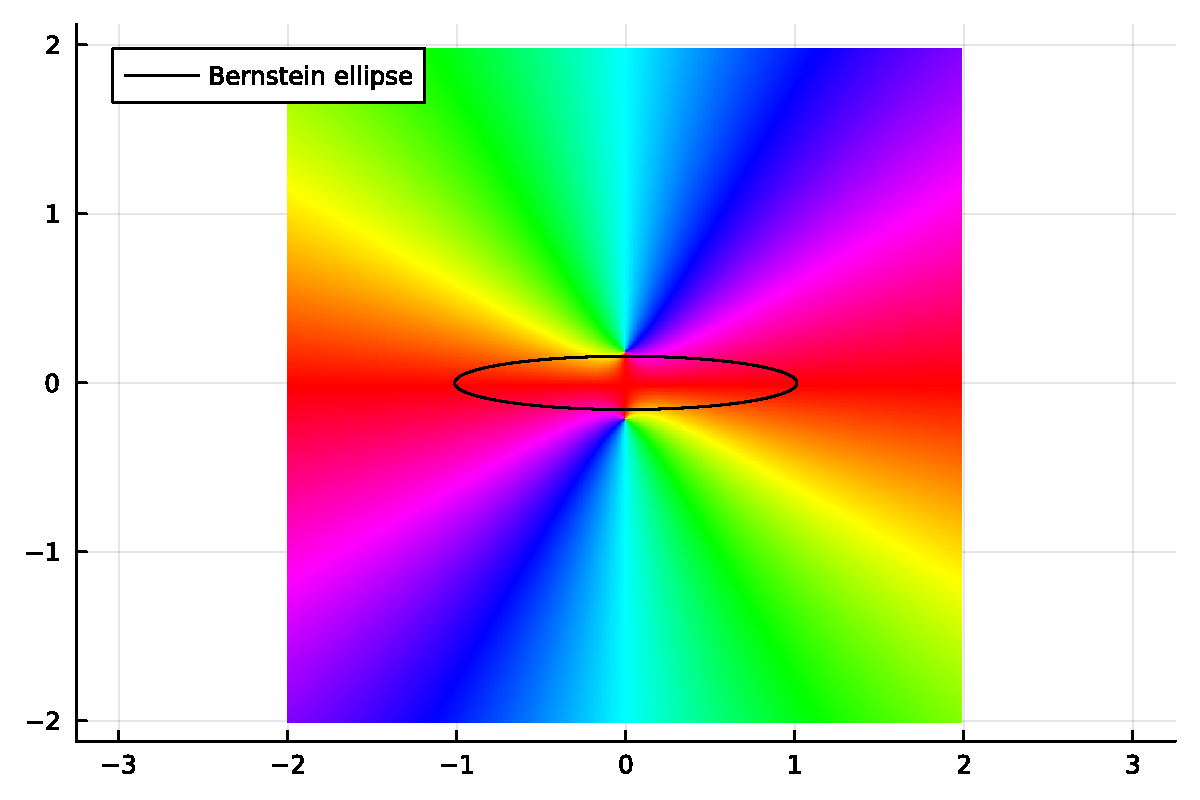
\includegraphics[width=\linewidth]{jl_dOthw0/OP_methods_26_1.pdf}

\begin{lstlisting}
(*@\HLJLnf{phaseplot}@*)(*@\HLJLp{(}@*)(*@\HLJLoB{-}@*)(*@\HLJLnfB{3..3}@*)(*@\HLJLp{,}@*) (*@\HLJLoB{-}@*)(*@\HLJLnfB{3..3}@*)(*@\HLJLp{,}@*) (*@\HLJLn{z}@*) (*@\HLJLoB{->}@*) (*@\HLJLnf{f}@*)(*@\HLJLp{((}@*)(*@\HLJLn{z}@*)(*@\HLJLoB{+}@*)(*@\HLJLni{1}@*)(*@\HLJLoB{/}@*)(*@\HLJLn{z}@*)(*@\HLJLp{)}@*)(*@\HLJLoB{/}@*)(*@\HLJLni{2}@*)(*@\HLJLp{))}@*)
(*@\HLJLnf{plot!}@*)(*@\HLJLp{(}@*)(*@\HLJLn{\ensuremath{\rho}}@*)(*@\HLJLoB{*}@*)(*@\HLJLn{cos}@*)(*@\HLJLoB{.}@*)(*@\HLJLp{(}@*)(*@\HLJLn{\ensuremath{\theta}}@*)(*@\HLJLp{),}@*)(*@\HLJLn{\ensuremath{\rho}}@*)(*@\HLJLoB{*}@*)(*@\HLJLn{sin}@*)(*@\HLJLoB{.}@*)(*@\HLJLp{(}@*)(*@\HLJLn{\ensuremath{\theta}}@*)(*@\HLJLp{),}@*)(*@\HLJLn{linecolor}@*)(*@\HLJLoB{=}@*)(*@\HLJLs{"{}black"{}}@*)(*@\HLJLp{,}@*)(*@\HLJLn{label}@*)(*@\HLJLoB{=}@*)(*@\HLJLs{"{}|z|}@*) (*@\HLJLs{=}@*) (*@\HLJLs{\ensuremath{\rho}"{}}@*)(*@\HLJLp{)}@*)
(*@\HLJLnf{plot!}@*)(*@\HLJLp{(}@*)(*@\HLJLn{cos}@*)(*@\HLJLoB{.}@*)(*@\HLJLp{(}@*)(*@\HLJLn{\ensuremath{\theta}}@*)(*@\HLJLp{)}@*)(*@\HLJLoB{/}@*)(*@\HLJLn{\ensuremath{\rho}}@*)(*@\HLJLp{,}@*)(*@\HLJLn{sin}@*)(*@\HLJLoB{.}@*)(*@\HLJLp{(}@*)(*@\HLJLn{\ensuremath{\theta}}@*)(*@\HLJLp{)}@*)(*@\HLJLoB{/}@*)(*@\HLJLn{\ensuremath{\rho}}@*)(*@\HLJLp{,}@*)(*@\HLJLn{linecolor}@*)(*@\HLJLoB{=}@*)(*@\HLJLs{"{}black"{}}@*)(*@\HLJLp{,}@*)(*@\HLJLn{label}@*)(*@\HLJLoB{=}@*)(*@\HLJLs{"{}|z|}@*) (*@\HLJLs{=}@*) (*@\HLJLs{1/\ensuremath{\rho}"{}}@*)(*@\HLJLp{)}@*)
\end{lstlisting}

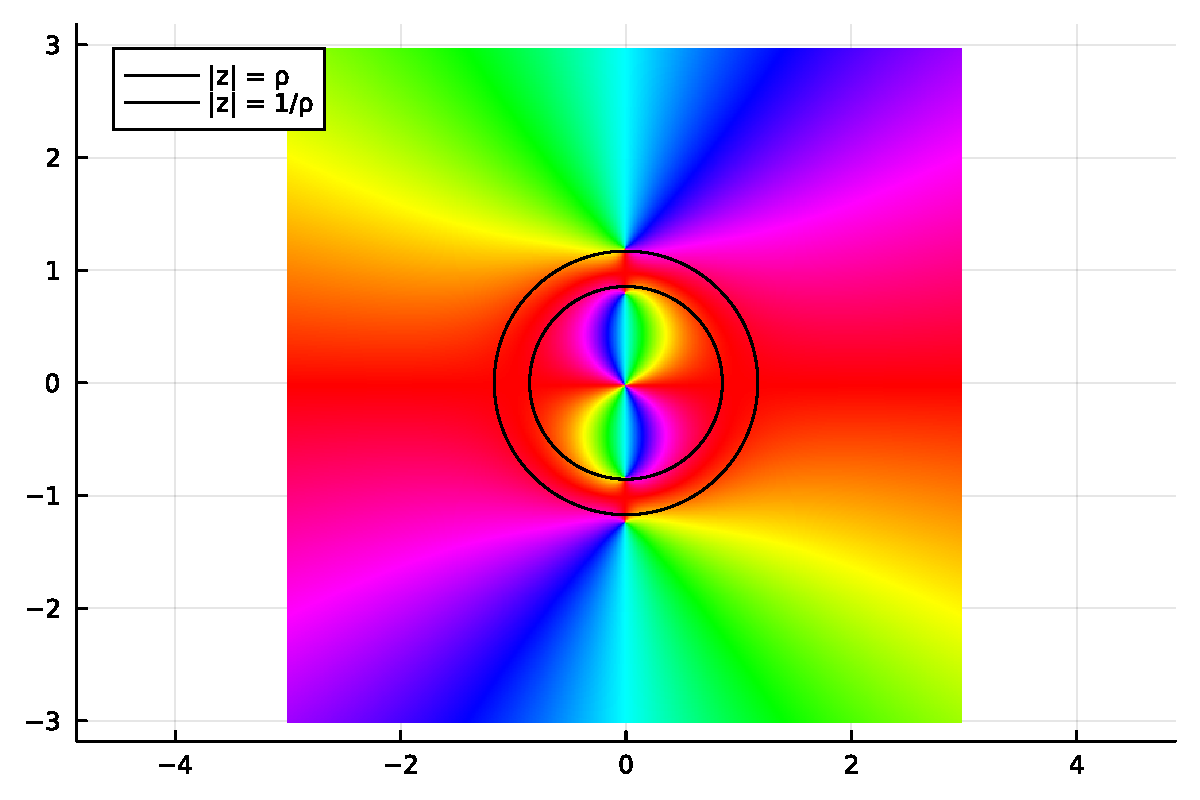
\includegraphics[width=\linewidth]{jl_dOthw0/OP_methods_27_1.pdf}

For $\beta = (\rho - \rho^{-1})/2 < 1/5$, we have

\[
M =  \sup_{x \in  E_{\rho}} |f(x)| = {1 \over 1 - 25 \beta^2}
\]
hence for $k \geq 1$,

\[
\vert f_k \vert \leq {2 \over   1 - 25 \beta^2} \rho^{-k}, \qquad 1 < \rho <  { 1 + \sqrt{26} \over 5 }.
\]
Therefore we predict a rate of decay of about $1.2198^{-k}$:


\begin{lstlisting}
(*@\HLJLnf{bound}@*)(*@\HLJLp{(}@*)(*@\HLJLn{\ensuremath{\beta}}@*)(*@\HLJLp{,}@*)(*@\HLJLn{k}@*)(*@\HLJLp{)}@*) (*@\HLJLoB{=}@*) (*@\HLJLni{2}@*)(*@\HLJLoB{/}@*)(*@\HLJLp{(}@*)(*@\HLJLni{1}@*)(*@\HLJLoB{-}@*)(*@\HLJLni{25}@*)(*@\HLJLoB{*}@*)(*@\HLJLn{\ensuremath{\beta}}@*)(*@\HLJLoB{{\textasciicircum}}@*)(*@\HLJLni{2}@*)(*@\HLJLp{)}@*)(*@\HLJLoB{*}@*)(*@\HLJLp{(}@*)(*@\HLJLn{\ensuremath{\beta}}@*) (*@\HLJLoB{+}@*) (*@\HLJLnf{sqrt}@*)(*@\HLJLp{(}@*)(*@\HLJLn{\ensuremath{\beta}}@*)(*@\HLJLoB{{\textasciicircum}}@*)(*@\HLJLni{2}@*) (*@\HLJLoB{+}@*) (*@\HLJLni{1}@*)(*@\HLJLp{))}@*)(*@\HLJLoB{{\textasciicircum}}@*)(*@\HLJLp{(}@*)(*@\HLJLoB{-}@*)(*@\HLJLn{k}@*)(*@\HLJLp{)}@*)
(*@\HLJLn{f}@*) (*@\HLJLoB{=}@*) (*@\HLJLnf{Fun}@*)(*@\HLJLp{(}@*) (*@\HLJLn{x}@*) (*@\HLJLoB{->}@*) (*@\HLJLni{1}@*)(*@\HLJLoB{/}@*)(*@\HLJLp{(}@*)(*@\HLJLni{25}@*)(*@\HLJLn{x}@*)(*@\HLJLoB{{\textasciicircum}}@*)(*@\HLJLni{2}@*) (*@\HLJLoB{+}@*) (*@\HLJLni{1}@*)(*@\HLJLp{),}@*) (*@\HLJLnf{Chebyshev}@*)(*@\HLJLp{())}@*)
(*@\HLJLnf{scatter}@*)(*@\HLJLp{(}@*)(*@\HLJLn{abs}@*)(*@\HLJLoB{.}@*)(*@\HLJLp{(}@*)(*@\HLJLn{f}@*)(*@\HLJLoB{.}@*)(*@\HLJLn{coefficients}@*)(*@\HLJLp{)}@*) (*@\HLJLoB{.+}@*) (*@\HLJLnf{eps}@*)(*@\HLJLp{();}@*) (*@\HLJLn{yscale}@*)(*@\HLJLoB{=:}@*)(*@\HLJLn{log10}@*)(*@\HLJLp{,}@*) (*@\HLJLn{label}@*)(*@\HLJLoB{=}@*)(*@\HLJLs{"{}Chebyshev}@*) (*@\HLJLs{coefficients"{}}@*)(*@\HLJLp{)}@*)
(*@\HLJLnf{plot!}@*)(*@\HLJLp{(}@*)(*@\HLJLni{1}@*)(*@\HLJLoB{:}@*)(*@\HLJLnf{ncoefficients}@*)(*@\HLJLp{(}@*)(*@\HLJLn{f}@*)(*@\HLJLp{),}@*) (*@\HLJLn{bound}@*)(*@\HLJLoB{.}@*)(*@\HLJLp{(}@*)(*@\HLJLni{1}@*)(*@\HLJLoB{/}@*)(*@\HLJLni{5}@*)(*@\HLJLoB{-}@*)(*@\HLJLnfB{0.001}@*)(*@\HLJLp{,}@*)(*@\HLJLni{1}@*)(*@\HLJLoB{:}@*)(*@\HLJLnf{ncoefficients}@*)(*@\HLJLp{(}@*)(*@\HLJLn{f}@*)(*@\HLJLp{));}@*) (*@\HLJLn{label}@*)(*@\HLJLoB{=}@*)(*@\HLJLs{"{}upper}@*) (*@\HLJLs{bound"{}}@*)(*@\HLJLp{)}@*)
(*@\HLJLcs{{\#}}@*) (*@\HLJLcs{Also}@*) (*@\HLJLcs{calculate}@*) (*@\HLJLcs{the}@*) (*@\HLJLcs{error}@*) (*@\HLJLcs{of}@*) (*@\HLJLcs{truncated}@*) (*@\HLJLcs{Chebyshev}@*) (*@\HLJLcs{expansions}@*) (*@\HLJLcs{with}@*) (*@\HLJLcs{n}@*) (*@\HLJLcs{terms}@*) (*@\HLJLcs{for}@*) (*@\HLJLcs{n}@*) (*@\HLJLcs{=}@*) (*@\HLJLcs{1,}@*) (*@\HLJLcs{2,}@*) (*@\HLJLcs{...}@*)
(*@\HLJLn{xx}@*) (*@\HLJLoB{=}@*) (*@\HLJLoB{-}@*)(*@\HLJLni{1}@*)(*@\HLJLoB{:}@*)(*@\HLJLnfB{0.001}@*)(*@\HLJLoB{:}@*)(*@\HLJLni{1}@*) (*@\HLJLcs{{\#}}@*) (*@\HLJLcs{a}@*) (*@\HLJLcs{fine}@*) (*@\HLJLcs{grid}@*) (*@\HLJLcs{on}@*) (*@\HLJLcs{which}@*) (*@\HLJLcs{to}@*) (*@\HLJLcs{evaluate}@*)
(*@\HLJLn{Errv}@*) (*@\HLJLoB{=}@*) (*@\HLJLp{[(}@*)(*@\HLJLnf{maximum}@*)(*@\HLJLp{(}@*)(*@\HLJLn{abs}@*)(*@\HLJLoB{.}@*)(*@\HLJLp{(}@*)(*@\HLJLn{f}@*)(*@\HLJLoB{.}@*)(*@\HLJLp{(}@*)(*@\HLJLn{xx}@*)(*@\HLJLp{)}@*)(*@\HLJLoB{-}@*)(*@\HLJLnf{Fun}@*)(*@\HLJLp{(}@*)(*@\HLJLn{f}@*)(*@\HLJLp{,}@*)(*@\HLJLnf{Chebyshev}@*)(*@\HLJLp{(),}@*)(*@\HLJLn{n}@*)(*@\HLJLp{)}@*)(*@\HLJLoB{.}@*)(*@\HLJLp{(}@*)(*@\HLJLn{xx}@*)(*@\HLJLp{))))}@*) (*@\HLJLk{for}@*) (*@\HLJLn{n}@*) (*@\HLJLoB{=}@*) (*@\HLJLni{1}@*)(*@\HLJLoB{:}@*)(*@\HLJLnf{ncoefficients}@*)(*@\HLJLp{(}@*)(*@\HLJLn{f}@*)(*@\HLJLp{)]}@*)
(*@\HLJLnf{scatter!}@*)(*@\HLJLp{(}@*)(*@\HLJLni{1}@*)(*@\HLJLoB{:}@*)(*@\HLJLnf{ncoefficients}@*)(*@\HLJLp{(}@*)(*@\HLJLn{f}@*)(*@\HLJLp{),}@*)(*@\HLJLn{Errv}@*)(*@\HLJLoB{.+}@*)(*@\HLJLnf{eps}@*)(*@\HLJLp{();}@*)(*@\HLJLn{label}@*)(*@\HLJLoB{=}@*)(*@\HLJLs{"{}truncated}@*) (*@\HLJLs{expansion}@*) (*@\HLJLs{error"{}}@*)(*@\HLJLp{)}@*)
(*@\HLJLnf{plot!}@*)(*@\HLJLp{(}@*) (*@\HLJLnfB{1.2198}@*)(*@\HLJLoB{.{\textasciicircum}}@*)(*@\HLJLp{(}@*)(*@\HLJLoB{-}@*)(*@\HLJLp{(}@*)(*@\HLJLni{0}@*)(*@\HLJLoB{:}@*)(*@\HLJLnf{ncoefficients}@*)(*@\HLJLp{(}@*)(*@\HLJLn{f}@*)(*@\HLJLp{)));}@*) (*@\HLJLn{label}@*)(*@\HLJLoB{=}@*)(*@\HLJLs{"{}\ensuremath{\rho}{\textasciicircum}(-k)"{}}@*)(*@\HLJLp{)}@*)
\end{lstlisting}

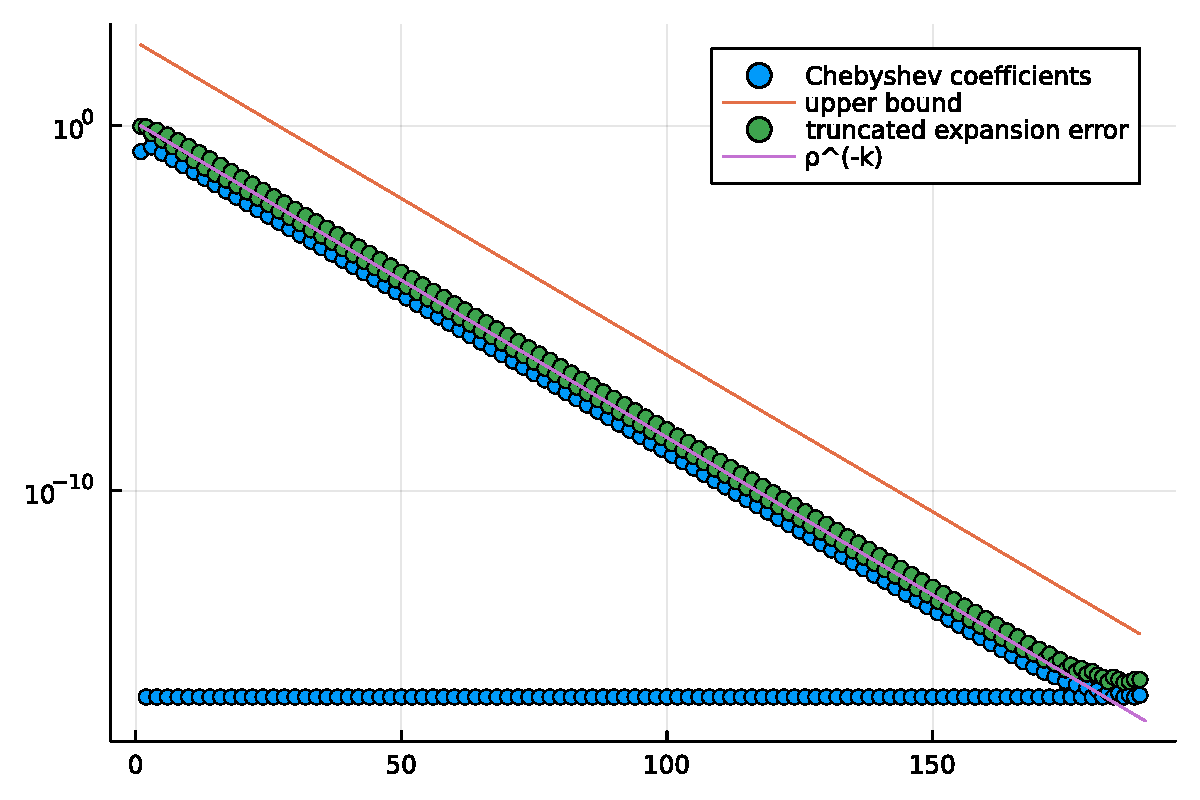
\includegraphics[width=\linewidth]{jl_dOthw0/OP_methods_28_1.pdf}

\textbf{Applied Complex Analysis (2021)}

\section{Lecture 20: Orthogonal polynomials and differential equations}
This lecture we do the following:

\begin{itemize}
\item[1. ] Recurrence relationships for Chebyshev and ultraspherical polynomials

\begin{itemize}
\item Conversion


\item Three-term recurrence and Jacobi operators

\end{itemize}

\item[2. ] Application: solving differential equations

\begin{itemize}
\item First order constant coefficients differential equations


\item Second order constant coefficient differential equations with boundary conditions


\item Non-constant coefficients

\end{itemize}

\item[3. ] Differential equations satisfied by orthogonal polynomials

\end{itemize}
That is, we introduce recurrences related to ultraspherical polynomials. This allows us to represent general linear differential equations as almost-banded systems.

\subsection{Recurrence relationships for Chebyshev and ultraspherical polynomials}
We have discussed general properties, but now we want to discuss some classical orthogonal polynomials, beginning with Chebyshev (first kind) $T_n(x)$, which is orthogonal w.r.t. $1\over \sqrt{1-x^2}$ and ultraspherical $C_n^{(\lambda)}(x)$, which is orthogonal w.r.t. $(1-x^2)^{\lambda - {1\over 2}}$ for $\lambda \rangle 0$. Note that Chebyshev (second kind) satisfies $U_n(x) = C_n^{(1)}(x)$.

For Chebyshev, recall we have the normalization constant (here we use a superscript $T_n(x) = k_n^{\rm T} x^n + O(x^{n-1})$)

\[
k_0^{\rm T} = 1, k_n^{\rm T} = 2^{n-1}
\]
For Ultraspherical $C_n^{(\lambda)}$, this is

\[
k_n^{(\lambda)} = {2^n (\lambda)_n \over n!} = {2^n \lambda (\lambda+1) (\lambda+2) \cdots (\lambda+n-1)  \over n!}
\]
where $(\lambda)_n$ is the Pochhammer symbol. Note for $U_n(x) = C_n^{(1)}(x)$ this simplifies to $k_n^{\rm U} = k_n^{(1)} = 2^n$.

We have  already found the recurrence for Chebyshev:

\[
x T_n(x) = {T_{n-1}(x) \over 2} +  {T_{n+1}(x) \over 2}
\]
We will show that we can use this to find the recurrence for \emph{all} ultraspherical polynomials. But first we need some special recurrences.

\textbf{Remark} Jacobi, Laguerre, and Hermite all have similar relationships, which will be discussed further in the problem sheet.

\subsubsection{Derivatives}
It turns out that the derivative of $T_n(x)$ is precisely a multiple of  $U_{n-1}(x)$, and similarly the derivative of $C_n^{(\lambda)}$ is a multiple of $C_{n-1}^{(\lambda+1)}$.

\textbf{Proposition (Chebyshev derivative)}

\[
T_n'(x) = n U_{n-1}(x)
\]
\textbf{Proof} We first show that $T_n'(x)$ is orthogonal w.r.t. $\sqrt{1-x^2}$ to all  polynomials of degree $m < n-1$, denoted $f_m$, using integration by parts:


\begin{align*}
\langle T_n',f_m\rangle_{\rm U} &= \int_{-1}^1 T_n'(x) f_m(x) \sqrt{1-x^2} {\rm d}x 
= -\int_{-1}^1 T_n(x) (f_m'(x)(1-x^2) - xf_m) {1  \over \sqrt{1-x^2}} {\rm d}x  
= - \langle T_n, f_m'(1-x^2) - x f_m \rangle_{\rm T}  = 0
\end{align*}
since $f_m'(1-x^2) - x f_m $ is degree $m-1 +2 = m+1 < n$.

The constant works out since

\[
T_n'(x) = {{\rm d} \over {\rm d}x} (2^{n-1} x^n)  + O(x^{n-2}) = n 2^{n-1} x^{n-1} + O(x^{n-2})
\]
\[
\blacksquare
\]
The exact same proof shows the following:

\textbf{Proposition (Ultraspherical derivative)} ${{\rm d} \over {\rm d}x} C_n^{(\lambda)}(x) = 2 \lambda  C_{n-1}^{(\lambda+1)}(x)$

Like the three-term recurrence and Jacobi operators, it is useful to express this in matrix form. That is, for the derivatives of $T_n(x)$ we get

\[
{{\rm d} \over {\rm d}x}  \begin{pmatrix} T_0(x) \\ T_1(x) \\ T_2(x) \\ \vdots \end{pmatrix}= \begin{pmatrix}
0 \cr
1 \cr
& 2 \cr
&& 3 \cr
&&&\ddots
\end{pmatrix} \begin{pmatrix} U_0(x) \\ U_1(x) \\ U_2(x) \\ \vdots \end{pmatrix}
\]
which lets us know that, for

\[
f(x) = (T_0(x),T_1(x),\ldots) \begin{pmatrix} f_0\\f_1\\\vdots \end{pmatrix}
\]
we have a derivative operator in coefficient space as

\[
f'(x) = (U_0(x),U_1(x),\ldots)\begin{pmatrix}
0 & 1 \cr
&& 2 \cr
&&& 3 \cr
&&&&\ddots
\end{pmatrix}  \begin{pmatrix} f_0\\f_1\\\vdots \end{pmatrix}
\]
\emph{Demonstration} Here we see that applying a matrix to a vector of coefficients successfully calculates the derivative:


\begin{lstlisting}
(*@\HLJLk{using}@*) (*@\HLJLn{ApproxFun}@*)(*@\HLJLp{,}@*) (*@\HLJLn{Plots}@*)(*@\HLJLp{,}@*) (*@\HLJLn{LinearAlgebra}@*)
(*@\HLJLn{f}@*) (*@\HLJLoB{=}@*) (*@\HLJLnf{Fun}@*)(*@\HLJLp{(}@*)(*@\HLJLn{x}@*) (*@\HLJLoB{->}@*) (*@\HLJLnf{cos}@*)(*@\HLJLp{(}@*)(*@\HLJLn{x}@*)(*@\HLJLoB{{\textasciicircum}}@*)(*@\HLJLni{2}@*)(*@\HLJLp{),}@*) (*@\HLJLnf{Chebyshev}@*)(*@\HLJLp{())}@*)   (*@\HLJLcs{{\#}}@*) (*@\HLJLcs{f}@*) (*@\HLJLcs{is}@*) (*@\HLJLcs{expanded}@*) (*@\HLJLcs{in}@*) (*@\HLJLcs{Chebyshev}@*) (*@\HLJLcs{coefficients}@*)
(*@\HLJLn{n}@*) (*@\HLJLoB{=}@*) (*@\HLJLnf{ncoefficients}@*)(*@\HLJLp{(}@*)(*@\HLJLn{f}@*)(*@\HLJLp{)}@*)   (*@\HLJLcs{{\#}}@*) (*@\HLJLcs{This}@*) (*@\HLJLcs{is}@*) (*@\HLJLcs{the}@*) (*@\HLJLcs{number}@*) (*@\HLJLcs{of}@*) (*@\HLJLcs{coefficients}@*)
(*@\HLJLn{D}@*) (*@\HLJLoB{=}@*) (*@\HLJLnf{zeros}@*)(*@\HLJLp{(}@*)(*@\HLJLn{n}@*)(*@\HLJLoB{-}@*)(*@\HLJLni{1}@*)(*@\HLJLp{,}@*)(*@\HLJLn{n}@*)(*@\HLJLp{)}@*)
(*@\HLJLk{for}@*) (*@\HLJLn{k}@*)(*@\HLJLoB{=}@*)(*@\HLJLni{1}@*)(*@\HLJLoB{:}@*)(*@\HLJLn{n}@*)(*@\HLJLoB{-}@*)(*@\HLJLni{1}@*)
    (*@\HLJLn{D}@*)(*@\HLJLp{[}@*)(*@\HLJLn{k}@*)(*@\HLJLp{,}@*)(*@\HLJLn{k}@*)(*@\HLJLoB{+}@*)(*@\HLJLni{1}@*)(*@\HLJLp{]}@*) (*@\HLJLoB{=}@*) (*@\HLJLn{k}@*)
(*@\HLJLk{end}@*)
(*@\HLJLn{D}@*)
\end{lstlisting}

\begin{lstlisting}
31(*@\ensuremath{\times}@*)32 Matrix(*@{{\{}}@*)Float64(*@{{\}}}@*):
 0.0  1.0  0.0  0.0  0.0  0.0  0.0  (*@\ensuremath{\ldots}@*)   0.0   0.0   0.0   0.0   0.0   0.0
 0.0  0.0  2.0  0.0  0.0  0.0  0.0      0.0   0.0   0.0   0.0   0.0   0.0
 0.0  0.0  0.0  3.0  0.0  0.0  0.0      0.0   0.0   0.0   0.0   0.0   0.0
 0.0  0.0  0.0  0.0  4.0  0.0  0.0      0.0   0.0   0.0   0.0   0.0   0.0
 0.0  0.0  0.0  0.0  0.0  5.0  0.0      0.0   0.0   0.0   0.0   0.0   0.0
 0.0  0.0  0.0  0.0  0.0  0.0  6.0  (*@\ensuremath{\ldots}@*)   0.0   0.0   0.0   0.0   0.0   0.0
 0.0  0.0  0.0  0.0  0.0  0.0  0.0      0.0   0.0   0.0   0.0   0.0   0.0
 0.0  0.0  0.0  0.0  0.0  0.0  0.0      0.0   0.0   0.0   0.0   0.0   0.0
 0.0  0.0  0.0  0.0  0.0  0.0  0.0      0.0   0.0   0.0   0.0   0.0   0.0
 0.0  0.0  0.0  0.0  0.0  0.0  0.0      0.0   0.0   0.0   0.0   0.0   0.0
 (*@\ensuremath{\vdots}@*)                        (*@\ensuremath{\vdots}@*)         (*@\ensuremath{\ddots}@*)                           (*@\ensuremath{\vdots}@*)    
 0.0  0.0  0.0  0.0  0.0  0.0  0.0      0.0   0.0   0.0   0.0   0.0   0.0
 0.0  0.0  0.0  0.0  0.0  0.0  0.0      0.0   0.0   0.0   0.0   0.0   0.0
 0.0  0.0  0.0  0.0  0.0  0.0  0.0      0.0   0.0   0.0   0.0   0.0   0.0
 0.0  0.0  0.0  0.0  0.0  0.0  0.0  (*@\ensuremath{\ldots}@*)  26.0   0.0   0.0   0.0   0.0   0.0
 0.0  0.0  0.0  0.0  0.0  0.0  0.0      0.0  27.0   0.0   0.0   0.0   0.0
 0.0  0.0  0.0  0.0  0.0  0.0  0.0      0.0   0.0  28.0   0.0   0.0   0.0
 0.0  0.0  0.0  0.0  0.0  0.0  0.0      0.0   0.0   0.0  29.0   0.0   0.0
 0.0  0.0  0.0  0.0  0.0  0.0  0.0      0.0   0.0   0.0   0.0  30.0   0.0
 0.0  0.0  0.0  0.0  0.0  0.0  0.0  (*@\ensuremath{\ldots}@*)   0.0   0.0   0.0   0.0   0.0  31.0
\end{lstlisting}


Here \texttt{D*f.coefficients} gives the vector of coefficients corresponding to the derivative, but now the coefficients are in the $U_n(x)$ basis, that is, \texttt{Ultraspherical(1)}:


\begin{lstlisting}
(*@\HLJLn{fp}@*) (*@\HLJLoB{=}@*) (*@\HLJLnf{Fun}@*)(*@\HLJLp{(}@*)(*@\HLJLnf{Ultraspherical}@*)(*@\HLJLp{(}@*)(*@\HLJLni{1}@*)(*@\HLJLp{),}@*) (*@\HLJLn{D}@*)(*@\HLJLoB{*}@*)(*@\HLJLn{f}@*)(*@\HLJLoB{.}@*)(*@\HLJLn{coefficients}@*)(*@\HLJLp{)}@*)
(*@\HLJLnf{fp}@*)(*@\HLJLp{(}@*)(*@\HLJLnfB{0.1}@*)(*@\HLJLp{)}@*)
\end{lstlisting}

\begin{lstlisting}
-0.001999966666833569
\end{lstlisting}


Indeed, it matches the "true" derivative:


\begin{lstlisting}
(*@\HLJLn{f}@*)(*@\HLJLoB{{\textquotesingle}}@*)(*@\HLJLp{(}@*)(*@\HLJLnfB{0.1}@*)(*@\HLJLp{),}@*)(*@\HLJLoB{-}@*)(*@\HLJLni{2}@*)(*@\HLJLoB{*}@*)(*@\HLJLnfB{0.1}@*)(*@\HLJLoB{*}@*)(*@\HLJLnf{sin}@*)(*@\HLJLp{(}@*)(*@\HLJLnfB{0.1}@*)(*@\HLJLoB{{\textasciicircum}}@*)(*@\HLJLni{2}@*)(*@\HLJLp{)}@*)
\end{lstlisting}

\begin{lstlisting}
(-0.0019999666668335634, -0.0019999666668333335)
\end{lstlisting}


Note that in ApproxFun.jl we can construct these operators rather nicely:


\begin{lstlisting}
(*@\HLJLn{D}@*) (*@\HLJLoB{=}@*) (*@\HLJLnf{Derivative}@*)(*@\HLJLp{()}@*)
(*@\HLJLp{(}@*)(*@\HLJLn{D}@*)(*@\HLJLoB{*}@*)(*@\HLJLn{f}@*)(*@\HLJLp{)(}@*)(*@\HLJLnfB{0.1}@*)(*@\HLJLp{)}@*)
\end{lstlisting}

\begin{lstlisting}
-0.001999966666833569
\end{lstlisting}


Here we see that we can produce the \ensuremath{\infty}-dimensional version as follows:


\begin{lstlisting}
(*@\HLJLn{D}@*) (*@\HLJLoB{:}@*) (*@\HLJLnf{Chebyshev}@*)(*@\HLJLp{()}@*) (*@\HLJLoB{\ensuremath{\rightarrow}}@*) (*@\HLJLnf{Ultraspherical}@*)(*@\HLJLp{(}@*)(*@\HLJLni{1}@*)(*@\HLJLp{)}@*)
\end{lstlisting}

\begin{lstlisting}
ConcreteDerivative : Chebyshev() (*@\ensuremath{\rightarrow}@*) Ultraspherical(1)
 (*@\ensuremath{\cdot}@*)  1.0   (*@\ensuremath{\cdot}@*)    (*@\ensuremath{\cdot}@*)    (*@\ensuremath{\cdot}@*)    (*@\ensuremath{\cdot}@*)    (*@\ensuremath{\cdot}@*)    (*@\ensuremath{\cdot}@*)    (*@\ensuremath{\cdot}@*)    (*@\ensuremath{\cdot}@*)   (*@\ensuremath{\cdot}@*)
 (*@\ensuremath{\cdot}@*)   (*@\ensuremath{\cdot}@*)   2.0   (*@\ensuremath{\cdot}@*)    (*@\ensuremath{\cdot}@*)    (*@\ensuremath{\cdot}@*)    (*@\ensuremath{\cdot}@*)    (*@\ensuremath{\cdot}@*)    (*@\ensuremath{\cdot}@*)    (*@\ensuremath{\cdot}@*)   (*@\ensuremath{\cdot}@*)
 (*@\ensuremath{\cdot}@*)   (*@\ensuremath{\cdot}@*)    (*@\ensuremath{\cdot}@*)   3.0   (*@\ensuremath{\cdot}@*)    (*@\ensuremath{\cdot}@*)    (*@\ensuremath{\cdot}@*)    (*@\ensuremath{\cdot}@*)    (*@\ensuremath{\cdot}@*)    (*@\ensuremath{\cdot}@*)   (*@\ensuremath{\cdot}@*)
 (*@\ensuremath{\cdot}@*)   (*@\ensuremath{\cdot}@*)    (*@\ensuremath{\cdot}@*)    (*@\ensuremath{\cdot}@*)   4.0   (*@\ensuremath{\cdot}@*)    (*@\ensuremath{\cdot}@*)    (*@\ensuremath{\cdot}@*)    (*@\ensuremath{\cdot}@*)    (*@\ensuremath{\cdot}@*)   (*@\ensuremath{\cdot}@*)
 (*@\ensuremath{\cdot}@*)   (*@\ensuremath{\cdot}@*)    (*@\ensuremath{\cdot}@*)    (*@\ensuremath{\cdot}@*)    (*@\ensuremath{\cdot}@*)   5.0   (*@\ensuremath{\cdot}@*)    (*@\ensuremath{\cdot}@*)    (*@\ensuremath{\cdot}@*)    (*@\ensuremath{\cdot}@*)   (*@\ensuremath{\cdot}@*)
 (*@\ensuremath{\cdot}@*)   (*@\ensuremath{\cdot}@*)    (*@\ensuremath{\cdot}@*)    (*@\ensuremath{\cdot}@*)    (*@\ensuremath{\cdot}@*)    (*@\ensuremath{\cdot}@*)   6.0   (*@\ensuremath{\cdot}@*)    (*@\ensuremath{\cdot}@*)    (*@\ensuremath{\cdot}@*)   (*@\ensuremath{\cdot}@*)
 (*@\ensuremath{\cdot}@*)   (*@\ensuremath{\cdot}@*)    (*@\ensuremath{\cdot}@*)    (*@\ensuremath{\cdot}@*)    (*@\ensuremath{\cdot}@*)    (*@\ensuremath{\cdot}@*)    (*@\ensuremath{\cdot}@*)   7.0   (*@\ensuremath{\cdot}@*)    (*@\ensuremath{\cdot}@*)   (*@\ensuremath{\cdot}@*)
 (*@\ensuremath{\cdot}@*)   (*@\ensuremath{\cdot}@*)    (*@\ensuremath{\cdot}@*)    (*@\ensuremath{\cdot}@*)    (*@\ensuremath{\cdot}@*)    (*@\ensuremath{\cdot}@*)    (*@\ensuremath{\cdot}@*)    (*@\ensuremath{\cdot}@*)   8.0   (*@\ensuremath{\cdot}@*)   (*@\ensuremath{\cdot}@*)
 (*@\ensuremath{\cdot}@*)   (*@\ensuremath{\cdot}@*)    (*@\ensuremath{\cdot}@*)    (*@\ensuremath{\cdot}@*)    (*@\ensuremath{\cdot}@*)    (*@\ensuremath{\cdot}@*)    (*@\ensuremath{\cdot}@*)    (*@\ensuremath{\cdot}@*)    (*@\ensuremath{\cdot}@*)   9.0  (*@\ensuremath{\cdot}@*)
 (*@\ensuremath{\cdot}@*)   (*@\ensuremath{\cdot}@*)    (*@\ensuremath{\cdot}@*)    (*@\ensuremath{\cdot}@*)    (*@\ensuremath{\cdot}@*)    (*@\ensuremath{\cdot}@*)    (*@\ensuremath{\cdot}@*)    (*@\ensuremath{\cdot}@*)    (*@\ensuremath{\cdot}@*)    (*@\ensuremath{\cdot}@*)   (*@\ensuremath{\ddots}@*)
 (*@\ensuremath{\cdot}@*)   (*@\ensuremath{\cdot}@*)    (*@\ensuremath{\cdot}@*)    (*@\ensuremath{\cdot}@*)    (*@\ensuremath{\cdot}@*)    (*@\ensuremath{\cdot}@*)    (*@\ensuremath{\cdot}@*)    (*@\ensuremath{\cdot}@*)    (*@\ensuremath{\cdot}@*)    (*@\ensuremath{\cdot}@*)   (*@\ensuremath{\ddots}@*)
\end{lstlisting}


\subsubsection{Conversion}
We can convert between any two polynomial bases using a lower triangular operator, because their spans are equivalent. In the case of Chebyshev and ultraspherical polynomials, they have the added property that they are banded.

\textbf{Proposition (Chebyshev T-to-U conversion)}


\begin{align*}
 T_0(x) &= U_0(x) \\
 T_1(x) &= {U_1(x) \over 2} \\
 T_n(x) &= {U_n(x) \over 2} - {U_{n-2}(x) \over 2}
\end{align*}
\textbf{Proof}

Before we do the proof, note that the fact that there are limited non-zero entries follows immediately: if $m < n-2$ we have

\[
\langle T_n, U_m\rangle_{\rm U} = \langle T_n, (1-x^2)U_m\rangle_{\rm T} = 0
\]
To actually determine the entries, we use the trigonometric formulae. Recall for $x = (z + z^{-1})/2$, $z = {\rm e}^{{\rm i} \theta}$, we have


\begin{align*}
T_n(x) &= \cos n \theta = {z^{-n} + z^n \over 2}\\
U_n(x) &= {\sin (n+1) \theta \over \sin \theta} = {z^{n+1} - z^{-n-1} \over z - z^{-1}} = z^{-n} + z^{2-n} + \cdots +  \cdots + z^{n-2} + z^n
\end{align*}
The result follows immediately.

\[
\blacksquare
\]
\textbf{Corollary (Ultraspherical \ensuremath{\lambda}-to-(\ensuremath{\lambda}+1) conversion)}

\[
C_n^{(\lambda)}(x) = {\lambda \over n+ \lambda} (C_n^{(\lambda+1)}(x) - C_{n-2}^{(\lambda+1)}(x))
\]
\textbf{Proof} This follows from differentiating the previous result. For example:


\begin{align*}
 {{\rm d} \over {\rm d}x} T_0(x) &= {{\rm d} \over {\rm d}x} U_0(x) \\
 {{\rm d} \over {\rm d}x} T_1(x) &= {{\rm d} \over {\rm d}x} {U_1(x) \over 2} \\
{{\rm d} \over {\rm d}x} T_n(x) &= {{\rm d} \over {\rm d}x} \left({U_n(x) \over 2} - {U_{n-2} \over 2} \right)
\end{align*}
becomes


\begin{align*}
    0 &= 0\\
    U_0(x) &= C_0^{(2)}(x) \\
   n U_{n-1}(x) &= C_{n-1}^{(2)}(x)  - C_{n-3}^{(2)}(x)
\end{align*}
Differentiating this repeatedly completes the proof.

\[
\blacksquare
\]
Note we can write this in matrix form, for example, we have

\[
\underbrace{\begin{pmatrix}1 \cr
                    0 & {1\over 2}\cr
                       -{1\over 2} & 0 & {1\over 2} \cr
                           &\ddots &\ddots & \ddots\end{pmatrix} }_{(R_T^U)^\top} \begin{pmatrix}
                           U_0(x) \\ U_1(x) \\ U_2(x) \\ \vdots \end{pmatrix}  =  \begin{pmatrix} T_0(x) \\ T_1(x) \\ T_2(x) \\ \vdots \end{pmatrix}
\]
therefore,

\[
f(x) =  (T_0(x),T_1(x),\ldots) \begin{pmatrix} f_0\\f_1\\\vdots \end{pmatrix} =  (U_0(x),U_1(x),\ldots) R_T^U \begin{pmatrix} f_0\\f_1\\\vdots \end{pmatrix}
\]
Again, we can construct this nicely in ApproxFun:


\begin{lstlisting}
(*@\HLJLn{R{\_}TU}@*) (*@\HLJLoB{=}@*) (*@\HLJLn{I}@*) (*@\HLJLoB{:}@*) (*@\HLJLnf{Chebyshev}@*)(*@\HLJLp{()}@*) (*@\HLJLoB{\ensuremath{\rightarrow}}@*) (*@\HLJLnf{Ultraspherical}@*)(*@\HLJLp{(}@*)(*@\HLJLni{1}@*)(*@\HLJLp{)}@*)

(*@\HLJLn{f}@*) (*@\HLJLoB{=}@*) (*@\HLJLnf{Fun}@*)(*@\HLJLp{(}@*)(*@\HLJLn{exp}@*)(*@\HLJLp{,}@*) (*@\HLJLnf{Chebyshev}@*)(*@\HLJLp{())}@*)
(*@\HLJLn{g}@*) (*@\HLJLoB{=}@*) (*@\HLJLn{R{\_}TU}@*)(*@\HLJLoB{*}@*)(*@\HLJLn{f}@*)

(*@\HLJLnf{g}@*)(*@\HLJLp{(}@*)(*@\HLJLnfB{0.1}@*)(*@\HLJLp{)}@*) (*@\HLJLp{,}@*) (*@\HLJLnf{exp}@*)(*@\HLJLp{(}@*)(*@\HLJLnfB{0.1}@*)(*@\HLJLp{)}@*)
\end{lstlisting}

\begin{lstlisting}
(1.1051709180756477, 1.1051709180756477)
\end{lstlisting}


\subsubsection{Ultraspherical Three-term recurrence}
\textbf{Theorem (three-term recurrence for Chebyshev U)}


\begin{align*}
x U_0(x) &= {U_1(x) \over 2} \\
x U_n(x) &= {U_{n-1}(x) \over 2} + {U_{n+1}(x) \over 2}
\end{align*}
\textbf{Proof} Differentiating


\begin{align*}
 x T_0(x) &= T_1(x) \\
x T_n(x)  &=  {T_{n-1}(x) \over 2} + {T_{n+1}(x) \over 2}
\end{align*}
we get


\begin{align*}
  T_0(x) &= U_0(x) \\
 T_n(x) + n x U_{n-1}(x)  &=  {(n-1) U_{n-2}(x) \over 2} + {(n+1) U_n(x) \over 2}
\end{align*}
substituting in the conversion $T_n(x) = (U_n(x) - U_{n-2}(x))/2$ we get


\begin{align*}
  T_0(x) &= U_0(x) \\
 n x U_{n-1}(x)  &=  {(n-1) U_{n-2}(x) \over 2} + {(n+1) U_n(x) \over 2} - (U_n(x) - U_{n-2}(x))/2 = {n U_{n-2}(x) \over 2} + {n U_n(x) \over 2}
\end{align*}
\[
\blacksquare
\]
Differentiating this theorem again and applying the conversion we get the following

\textbf{Corollary (three-term recurrence for ultraspherical)}


\begin{align*}
x C_0^{(\lambda)}(x) &= {1 \over 2\lambda } C_1^{(\lambda)}(x) \\
 x C_n^{(\lambda)}(x) &=  {n+2\lambda-1 \over 2(n+\lambda)} C_{n-1}^{(\lambda)}(x) + {n+1 \over 2(n+\lambda)} C_{n+1}^{(\lambda)}(x)
\end{align*}
Here's an example of the Jacobi operator (which is the transpose of the multiplication by $x$ operator):


\begin{lstlisting}
(*@\HLJLnf{Multiplication}@*)(*@\HLJLp{(}@*)(*@\HLJLnf{Fun}@*)(*@\HLJLp{(),}@*) (*@\HLJLnf{Ultraspherical}@*)(*@\HLJLp{(}@*)(*@\HLJLni{2}@*)(*@\HLJLp{))}@*)(*@\HLJLoB{{\textquotesingle}}@*)
\end{lstlisting}

\begin{lstlisting}
AdjointOperator : Ultraspherical(2) (*@\ensuremath{\rightarrow}@*) Ultraspherical(2)
 0.0                 0.25   (*@\ensuremath{\ldots}@*)   (*@\ensuremath{\cdot}@*)       (*@\ensuremath{\cdot}@*)                   (*@\ensuremath{\cdot}@*)    (*@\ensuremath{\cdot}@*)
 0.6666666666666666  0.0        (*@\ensuremath{\cdot}@*)       (*@\ensuremath{\cdot}@*)                   (*@\ensuremath{\cdot}@*)    (*@\ensuremath{\cdot}@*)
  (*@\ensuremath{\cdot}@*)                  0.625      (*@\ensuremath{\cdot}@*)       (*@\ensuremath{\cdot}@*)                   (*@\ensuremath{\cdot}@*)    (*@\ensuremath{\cdot}@*)
  (*@\ensuremath{\cdot}@*)                   (*@\ensuremath{\cdot}@*)         (*@\ensuremath{\cdot}@*)       (*@\ensuremath{\cdot}@*)                   (*@\ensuremath{\cdot}@*)    (*@\ensuremath{\cdot}@*)
  (*@\ensuremath{\cdot}@*)                   (*@\ensuremath{\cdot}@*)         (*@\ensuremath{\cdot}@*)       (*@\ensuremath{\cdot}@*)                   (*@\ensuremath{\cdot}@*)    (*@\ensuremath{\cdot}@*)
  (*@\ensuremath{\cdot}@*)                   (*@\ensuremath{\cdot}@*)     (*@\ensuremath{\ldots}@*)   (*@\ensuremath{\cdot}@*)       (*@\ensuremath{\cdot}@*)                   (*@\ensuremath{\cdot}@*)    (*@\ensuremath{\cdot}@*)
  (*@\ensuremath{\cdot}@*)                   (*@\ensuremath{\cdot}@*)        0.4375   (*@\ensuremath{\cdot}@*)                   (*@\ensuremath{\cdot}@*)    (*@\ensuremath{\cdot}@*)
  (*@\ensuremath{\cdot}@*)                   (*@\ensuremath{\cdot}@*)        0.0     0.4444444444444444   (*@\ensuremath{\cdot}@*)    (*@\ensuremath{\cdot}@*)
  (*@\ensuremath{\cdot}@*)                   (*@\ensuremath{\cdot}@*)        0.55    0.0                 0.45  (*@\ensuremath{\cdot}@*)
  (*@\ensuremath{\cdot}@*)                   (*@\ensuremath{\cdot}@*)         (*@\ensuremath{\cdot}@*)      0.5454545454545454  0.0   (*@\ensuremath{\ddots}@*)
  (*@\ensuremath{\cdot}@*)                   (*@\ensuremath{\cdot}@*)     (*@\ensuremath{\ldots}@*)   (*@\ensuremath{\cdot}@*)       (*@\ensuremath{\cdot}@*)                   (*@\ensuremath{\ddots}@*)    (*@\ensuremath{\ddots}@*)
\end{lstlisting}


\subsection{Application: solving differential equations}
The preceding results allowed us to represent

\begin{itemize}
\item[1. ] Differentiation


\item[2. ] Conversion


\item[3. ] Multiplication

\end{itemize}
as banded operators. We will see that we can combine these, along with

\begin{itemize}
\item[4. ] Evaluation

\end{itemize}
to solve ordinary differential equations.

\subsubsection{First order, constant coefficient differential equations}
Consider the simplest ODE:


\begin{align*}
u(0) &= 1 \\
u'(x) - u(x) &= 0, \qquad x \in [-1, 1]
\end{align*}
and suppose we represent $u(x)$ in its Chebyshev expansion, with coefficients to be determined. In other words, we want to calculate coefficients $u_k$ such that

\[
u(x) = \sum_{k=0}^\infty u_k T_k(x) = (T_0(x), T_1(x), \ldots) \begin{pmatrix} u_0 \\ u_1 \\ \vdots \end{pmatrix}
\]
In this case we know that $u(x) = {\rm e}^x$, but we would still need other means to calculate $u_k$ (They are definitely not as simple as Taylor series coefficients).

We can express the constraints as acting on the coefficients. For example, we have

\[
u(0) = (T_0(0), T_1(0), \ldots) \begin{pmatrix} u_0\\u_1\\\vdots \end{pmatrix} = (1,0,-1,0,1,\ldots)  \begin{pmatrix} u_0\\u_1\\\vdots \end{pmatrix}
\]
We also have

\[
u'(x) = (U_0(x),U_1(x),\ldots) \begin{pmatrix}
0 & 1 \cr
&& 2 \cr
&&& 3 \cr
&&&&\ddots
\end{pmatrix}\begin{pmatrix} u_0\\u_1\\\vdots \end{pmatrix}
\]
To represent $u'(x) - u(x)$, we need to make sure the bases are compatible. In other words, we want to express $u(x)$ in its $U_k(x)$ basis using the conversion operator $R_T^{U}$:

\[
u(x) = (U_0(x),U_1(x),\ldots) \begin{pmatrix}
    1 &0 & -{1 \over 2} \cr
& {1 \over 2} & 0 & -{1 \over 2} \cr
&&\ddots & \ddots & \ddots
\end{pmatrix}\begin{pmatrix} u_0\\u_1\\\vdots \end{pmatrix}
\]
Which gives us,

\[
u'(x) - u(x) =  (U_0(x),U_1(x),\ldots)  \begin{pmatrix}
    -1 &1 & {1 \over 2} \cr
& -{1 \over 2} & 2 & {1 \over 2} \cr
&& -{1 \over 2} & 3 & {1 \over 2} \cr
&&&\ddots & \ddots & \ddots
\end{pmatrix} \begin{pmatrix} u_0\\u_1\\\vdots \end{pmatrix}
\]
Combing the differential part and the evaluation part, we arrive at an (infinite) system of equations for the coefficients $u_0,u_1,\dots$:

\[
\begin{pmatrix}
      1 & 0 & -1 & 0 & 1 & \cdots \\
    -1 &1 & {1 \over 2} \cr
& -{1 \over 2} & 2 & {1 \over 2} \cr
&& -{1 \over 2} & 3 & {1 \over 2} \cr
&&&\ddots & \ddots & \ddots
\end{pmatrix} \begin{pmatrix} u_0\\u_1\\\vdots \end{pmatrix}  = \begin{pmatrix} 1 \\ 0 \\ 0 \\ \vdots \end{pmatrix}
\]
How to solve this system is outside the scope of this course (though a simple approach is to truncate the infinite system to finite systems). We can however do this in ApproxFun:


\begin{lstlisting}
(*@\HLJLn{B}@*)  (*@\HLJLoB{=}@*) (*@\HLJLnf{Evaluation}@*)(*@\HLJLp{(}@*)(*@\HLJLnfB{0.0}@*)(*@\HLJLp{)}@*) (*@\HLJLoB{:}@*) (*@\HLJLnf{Chebyshev}@*)(*@\HLJLp{()}@*)
(*@\HLJLn{D}@*)  (*@\HLJLoB{=}@*) (*@\HLJLnf{Derivative}@*)(*@\HLJLp{()}@*) (*@\HLJLoB{:}@*) (*@\HLJLnf{Chebyshev}@*)(*@\HLJLp{()}@*) (*@\HLJLoB{\ensuremath{\rightarrow}}@*) (*@\HLJLnf{Ultraspherical}@*)(*@\HLJLp{(}@*)(*@\HLJLni{1}@*)(*@\HLJLp{)}@*)
(*@\HLJLn{R{\_}TU}@*) (*@\HLJLoB{=}@*) (*@\HLJLn{I}@*) (*@\HLJLoB{:}@*) (*@\HLJLnf{Chebyshev}@*)(*@\HLJLp{()}@*) (*@\HLJLoB{\ensuremath{\rightarrow}}@*) (*@\HLJLnf{Ultraspherical}@*)(*@\HLJLp{(}@*)(*@\HLJLni{1}@*)(*@\HLJLp{)}@*)
(*@\HLJLn{L}@*) (*@\HLJLoB{=}@*) (*@\HLJLp{[}@*)(*@\HLJLn{B}@*)(*@\HLJLp{;}@*)
     (*@\HLJLn{D}@*) (*@\HLJLoB{-}@*) (*@\HLJLn{R{\_}TU}@*)(*@\HLJLp{]}@*)
\end{lstlisting}

\begin{lstlisting}
InterlaceOperator : Chebyshev() (*@\ensuremath{\rightarrow}@*) 2-element ArraySpace:
Space(*@{{\{}}@*)D, Float64(*@{{\}}}@*) where D[ConstantSpace(Point(0.0)), Ultraspherical(1)]
  1.0   0.0  -1.0   0.0   1.0   0.0  -1.0   0.0   1.0  0.0  (*@\ensuremath{\cdots}@*)
 -1.0   1.0   0.5   0.0   0.0   0.0   0.0   0.0   0.0  0.0  (*@\ensuremath{\ddots}@*)
  0.0  -0.5   2.0   0.5   0.0   0.0   0.0   0.0   0.0  0.0  (*@\ensuremath{\ddots}@*)
  0.0   0.0  -0.5   3.0   0.5   0.0   0.0   0.0   0.0  0.0  (*@\ensuremath{\ddots}@*)
  0.0   0.0   0.0  -0.5   4.0   0.5   0.0   0.0   0.0  0.0  (*@\ensuremath{\ddots}@*)
  0.0   0.0   0.0   0.0  -0.5   5.0   0.5   0.0   0.0  0.0  (*@\ensuremath{\ddots}@*)
  0.0   0.0   0.0   0.0   0.0  -0.5   6.0   0.5   0.0  0.0  (*@\ensuremath{\ddots}@*)
  0.0   0.0   0.0   0.0   0.0   0.0  -0.5   7.0   0.5  0.0  (*@\ensuremath{\ddots}@*)
  0.0   0.0   0.0   0.0   0.0   0.0   0.0  -0.5   8.0  0.5  (*@\ensuremath{\ddots}@*)
  0.0   0.0   0.0   0.0   0.0   0.0   0.0   0.0  -0.5  9.0  (*@\ensuremath{\ddots}@*)
   (*@\ensuremath{\vdots}@*)     (*@\ensuremath{\ddots}@*)     (*@\ensuremath{\ddots}@*)     (*@\ensuremath{\ddots}@*)     (*@\ensuremath{\ddots}@*)     (*@\ensuremath{\ddots}@*)     (*@\ensuremath{\ddots}@*)     (*@\ensuremath{\ddots}@*)     (*@\ensuremath{\ddots}@*)    (*@\ensuremath{\ddots}@*)   (*@\ensuremath{\ddots}@*)
\end{lstlisting}


We can solve this system as follows:


\begin{lstlisting}
(*@\HLJLn{u}@*) (*@\HLJLoB{=}@*) (*@\HLJLn{L}@*) (*@\HLJLoB{{\textbackslash}}@*) (*@\HLJLp{[}@*)(*@\HLJLni{1}@*)(*@\HLJLp{;}@*) (*@\HLJLni{0}@*)(*@\HLJLp{]}@*)
(*@\HLJLnf{plot}@*)(*@\HLJLp{(}@*)(*@\HLJLn{u}@*)(*@\HLJLp{;}@*)(*@\HLJLn{legend}@*)(*@\HLJLoB{=}@*)(*@\HLJLkc{false}@*)(*@\HLJLp{)}@*)
\end{lstlisting}

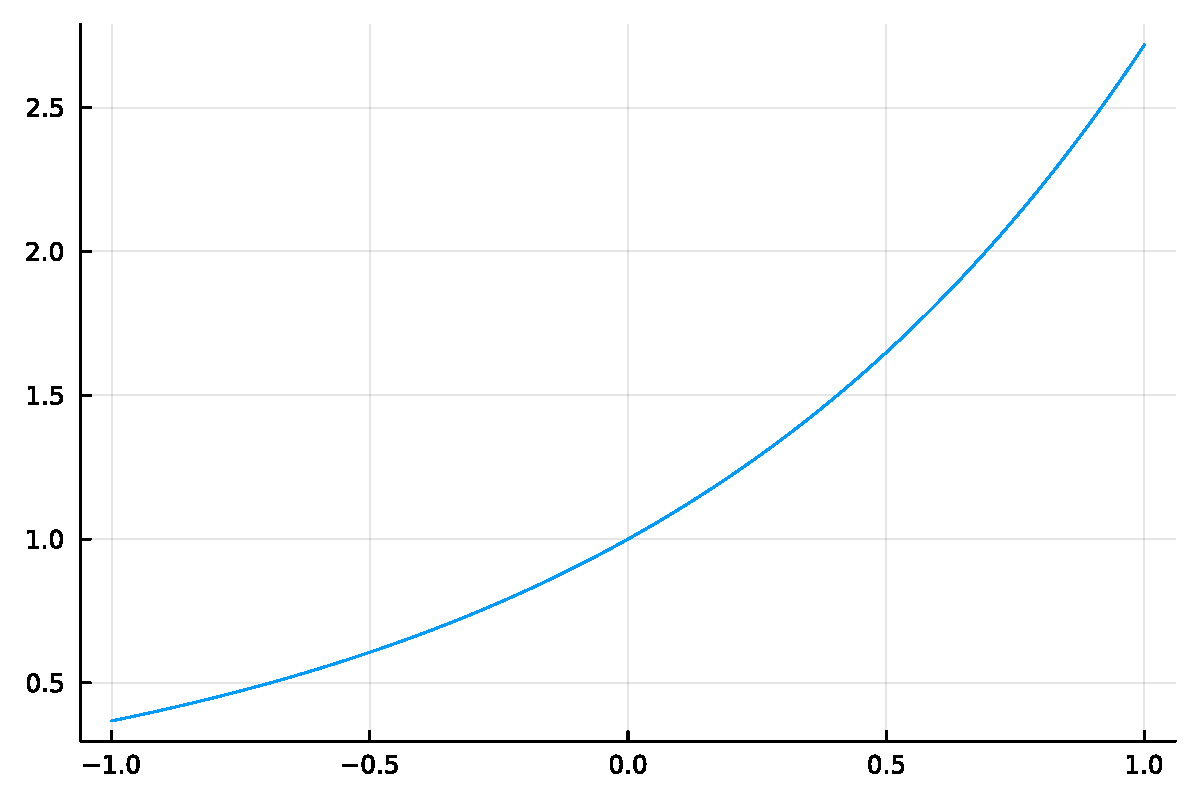
\includegraphics[width=\linewidth]{jl_dOthw0/OP_methods_37_1.pdf}

It matches the "true" result:

Note we can incorporate right-hand sides as well, for example, to solve $u'(x) - u(x) = f(x)$, by expanding $f$ in its Chebyshev U series.

\subsubsection{Second-order constant coefficient equations}
This approach extends to second-order constant-coefficient equations by using ultraspherical polynomials.  Consider


\begin{align*}
u(-1) &= 1\\
u(1) &= 0\\
u''(x) + u'(x)  + u(x) &= 0
\end{align*}
Evaluation works as in the first-order case. To handle second-derivatives, we need $C^{(2)}$ polynomials:


\begin{lstlisting}
(*@\HLJLn{D\ensuremath{\_0}}@*) (*@\HLJLoB{=}@*) (*@\HLJLnf{Derivative}@*)(*@\HLJLp{()}@*) (*@\HLJLoB{:}@*) (*@\HLJLnf{Chebyshev}@*)(*@\HLJLp{()}@*) (*@\HLJLoB{\ensuremath{\rightarrow}}@*) (*@\HLJLnf{Ultraspherical}@*)(*@\HLJLp{(}@*)(*@\HLJLni{1}@*)(*@\HLJLp{)}@*)
(*@\HLJLn{D\ensuremath{\_1}}@*) (*@\HLJLoB{=}@*) (*@\HLJLnf{Derivative}@*)(*@\HLJLp{()}@*) (*@\HLJLoB{:}@*) (*@\HLJLnf{Ultraspherical}@*)(*@\HLJLp{(}@*)(*@\HLJLni{1}@*)(*@\HLJLp{)}@*) (*@\HLJLoB{\ensuremath{\rightarrow}}@*) (*@\HLJLnf{Ultraspherical}@*)(*@\HLJLp{(}@*)(*@\HLJLni{2}@*)(*@\HLJLp{)}@*)
(*@\HLJLn{D\ensuremath{\_1}}@*)(*@\HLJLoB{*}@*)(*@\HLJLn{D\ensuremath{\_0}}@*)  (*@\HLJLcs{{\#}}@*) (*@\HLJLcs{2}@*) (*@\HLJLcs{zeros}@*) (*@\HLJLcs{not}@*) (*@\HLJLcs{printed}@*) (*@\HLJLcs{in}@*) (*@\HLJLcs{(1,1)}@*) (*@\HLJLcs{and}@*) (*@\HLJLcs{(1,2)}@*) (*@\HLJLcs{entry}@*)
\end{lstlisting}

\begin{lstlisting}
ConcreteDerivative : Chebyshev() (*@\ensuremath{\rightarrow}@*) Ultraspherical(2)
 (*@\ensuremath{\cdot}@*)  (*@\ensuremath{\cdot}@*)  4.0   (*@\ensuremath{\cdot}@*)    (*@\ensuremath{\cdot}@*)     (*@\ensuremath{\cdot}@*)     (*@\ensuremath{\cdot}@*)     (*@\ensuremath{\cdot}@*)     (*@\ensuremath{\cdot}@*)     (*@\ensuremath{\cdot}@*)   (*@\ensuremath{\cdot}@*)
 (*@\ensuremath{\cdot}@*)  (*@\ensuremath{\cdot}@*)   (*@\ensuremath{\cdot}@*)   6.0   (*@\ensuremath{\cdot}@*)     (*@\ensuremath{\cdot}@*)     (*@\ensuremath{\cdot}@*)     (*@\ensuremath{\cdot}@*)     (*@\ensuremath{\cdot}@*)     (*@\ensuremath{\cdot}@*)   (*@\ensuremath{\cdot}@*)
 (*@\ensuremath{\cdot}@*)  (*@\ensuremath{\cdot}@*)   (*@\ensuremath{\cdot}@*)    (*@\ensuremath{\cdot}@*)   8.0    (*@\ensuremath{\cdot}@*)     (*@\ensuremath{\cdot}@*)     (*@\ensuremath{\cdot}@*)     (*@\ensuremath{\cdot}@*)     (*@\ensuremath{\cdot}@*)   (*@\ensuremath{\cdot}@*)
 (*@\ensuremath{\cdot}@*)  (*@\ensuremath{\cdot}@*)   (*@\ensuremath{\cdot}@*)    (*@\ensuremath{\cdot}@*)    (*@\ensuremath{\cdot}@*)   10.0    (*@\ensuremath{\cdot}@*)     (*@\ensuremath{\cdot}@*)     (*@\ensuremath{\cdot}@*)     (*@\ensuremath{\cdot}@*)   (*@\ensuremath{\cdot}@*)
 (*@\ensuremath{\cdot}@*)  (*@\ensuremath{\cdot}@*)   (*@\ensuremath{\cdot}@*)    (*@\ensuremath{\cdot}@*)    (*@\ensuremath{\cdot}@*)     (*@\ensuremath{\cdot}@*)   12.0    (*@\ensuremath{\cdot}@*)     (*@\ensuremath{\cdot}@*)     (*@\ensuremath{\cdot}@*)   (*@\ensuremath{\cdot}@*)
 (*@\ensuremath{\cdot}@*)  (*@\ensuremath{\cdot}@*)   (*@\ensuremath{\cdot}@*)    (*@\ensuremath{\cdot}@*)    (*@\ensuremath{\cdot}@*)     (*@\ensuremath{\cdot}@*)     (*@\ensuremath{\cdot}@*)   14.0    (*@\ensuremath{\cdot}@*)     (*@\ensuremath{\cdot}@*)   (*@\ensuremath{\cdot}@*)
 (*@\ensuremath{\cdot}@*)  (*@\ensuremath{\cdot}@*)   (*@\ensuremath{\cdot}@*)    (*@\ensuremath{\cdot}@*)    (*@\ensuremath{\cdot}@*)     (*@\ensuremath{\cdot}@*)     (*@\ensuremath{\cdot}@*)     (*@\ensuremath{\cdot}@*)   16.0    (*@\ensuremath{\cdot}@*)   (*@\ensuremath{\cdot}@*)
 (*@\ensuremath{\cdot}@*)  (*@\ensuremath{\cdot}@*)   (*@\ensuremath{\cdot}@*)    (*@\ensuremath{\cdot}@*)    (*@\ensuremath{\cdot}@*)     (*@\ensuremath{\cdot}@*)     (*@\ensuremath{\cdot}@*)     (*@\ensuremath{\cdot}@*)     (*@\ensuremath{\cdot}@*)   18.0  (*@\ensuremath{\cdot}@*)
 (*@\ensuremath{\cdot}@*)  (*@\ensuremath{\cdot}@*)   (*@\ensuremath{\cdot}@*)    (*@\ensuremath{\cdot}@*)    (*@\ensuremath{\cdot}@*)     (*@\ensuremath{\cdot}@*)     (*@\ensuremath{\cdot}@*)     (*@\ensuremath{\cdot}@*)     (*@\ensuremath{\cdot}@*)     (*@\ensuremath{\cdot}@*)   (*@\ensuremath{\ddots}@*)
 (*@\ensuremath{\cdot}@*)  (*@\ensuremath{\cdot}@*)   (*@\ensuremath{\cdot}@*)    (*@\ensuremath{\cdot}@*)    (*@\ensuremath{\cdot}@*)     (*@\ensuremath{\cdot}@*)     (*@\ensuremath{\cdot}@*)     (*@\ensuremath{\cdot}@*)     (*@\ensuremath{\cdot}@*)     (*@\ensuremath{\cdot}@*)   (*@\ensuremath{\ddots}@*)
 (*@\ensuremath{\cdot}@*)  (*@\ensuremath{\cdot}@*)   (*@\ensuremath{\cdot}@*)    (*@\ensuremath{\cdot}@*)    (*@\ensuremath{\cdot}@*)     (*@\ensuremath{\cdot}@*)     (*@\ensuremath{\cdot}@*)     (*@\ensuremath{\cdot}@*)     (*@\ensuremath{\cdot}@*)     (*@\ensuremath{\cdot}@*)   (*@\ensuremath{\ddots}@*)
\end{lstlisting}


For the identity operator, we use two conversion operators:


\begin{lstlisting}
(*@\HLJLn{R{\_}TU}@*) (*@\HLJLoB{=}@*) (*@\HLJLn{I}@*) (*@\HLJLoB{:}@*) (*@\HLJLnf{Chebyshev}@*)(*@\HLJLp{()}@*) (*@\HLJLoB{\ensuremath{\rightarrow}}@*) (*@\HLJLnf{Ultraspherical}@*)(*@\HLJLp{(}@*)(*@\HLJLni{1}@*)(*@\HLJLp{)}@*)
(*@\HLJLn{R{\_}U2}@*) (*@\HLJLoB{=}@*) (*@\HLJLn{I}@*) (*@\HLJLoB{:}@*) (*@\HLJLnf{Ultraspherical}@*)(*@\HLJLp{(}@*)(*@\HLJLni{1}@*)(*@\HLJLp{)}@*) (*@\HLJLoB{\ensuremath{\rightarrow}}@*) (*@\HLJLnf{Ultraspherical}@*)(*@\HLJLp{(}@*)(*@\HLJLni{2}@*)(*@\HLJLp{)}@*)
(*@\HLJLn{R{\_}T2}@*) (*@\HLJLoB{=}@*) (*@\HLJLn{R{\_}U2}@*)(*@\HLJLoB{*}@*)(*@\HLJLn{R{\_}TU}@*)
\end{lstlisting}

\begin{lstlisting}
TimesOperator : Chebyshev() (*@\ensuremath{\rightarrow}@*) Ultraspherical(2)
 1.0  0.0   -0.6666666666666666    0.0    (*@\ensuremath{\ldots}@*)    (*@\ensuremath{\cdot}@*)                     (*@\ensuremath{\cdot}@*)     
 (*@\ensuremath{\cdot}@*)
  (*@\ensuremath{\cdot}@*)   0.25   0.0                  -0.375       (*@\ensuremath{\cdot}@*)                     (*@\ensuremath{\cdot}@*)     
 (*@\ensuremath{\cdot}@*)
  (*@\ensuremath{\cdot}@*)    (*@\ensuremath{\cdot}@*)     0.16666666666666666   0.0         (*@\ensuremath{\cdot}@*)                     (*@\ensuremath{\cdot}@*)     
 (*@\ensuremath{\cdot}@*)
  (*@\ensuremath{\cdot}@*)    (*@\ensuremath{\cdot}@*)      (*@\ensuremath{\cdot}@*)                    0.125       (*@\ensuremath{\cdot}@*)                     (*@\ensuremath{\cdot}@*)     
 (*@\ensuremath{\cdot}@*)
  (*@\ensuremath{\cdot}@*)    (*@\ensuremath{\cdot}@*)      (*@\ensuremath{\cdot}@*)                     (*@\ensuremath{\cdot}@*)         0.07142857142857142    (*@\ensuremath{\cdot}@*)     
 (*@\ensuremath{\cdot}@*)
  (*@\ensuremath{\cdot}@*)    (*@\ensuremath{\cdot}@*)      (*@\ensuremath{\cdot}@*)                     (*@\ensuremath{\cdot}@*)     (*@\ensuremath{\ldots}@*)   0.0                   0.0625 
 (*@\ensuremath{\cdot}@*)
  (*@\ensuremath{\cdot}@*)    (*@\ensuremath{\cdot}@*)      (*@\ensuremath{\cdot}@*)                     (*@\ensuremath{\cdot}@*)        -0.12698412698412698   0.0    
 (*@\ensuremath{\ddots}@*)
  (*@\ensuremath{\cdot}@*)    (*@\ensuremath{\cdot}@*)      (*@\ensuremath{\cdot}@*)                     (*@\ensuremath{\cdot}@*)         0.0                  -0.1125 
 (*@\ensuremath{\ddots}@*)
  (*@\ensuremath{\cdot}@*)    (*@\ensuremath{\cdot}@*)      (*@\ensuremath{\cdot}@*)                     (*@\ensuremath{\cdot}@*)         0.05555555555555555   0.0    
 (*@\ensuremath{\ddots}@*)
  (*@\ensuremath{\cdot}@*)    (*@\ensuremath{\cdot}@*)      (*@\ensuremath{\cdot}@*)                     (*@\ensuremath{\cdot}@*)          (*@\ensuremath{\cdot}@*)                    0.05   
 (*@\ensuremath{\ddots}@*)
  (*@\ensuremath{\cdot}@*)    (*@\ensuremath{\cdot}@*)      (*@\ensuremath{\cdot}@*)                     (*@\ensuremath{\cdot}@*)     (*@\ensuremath{\ldots}@*)    (*@\ensuremath{\cdot}@*)                     (*@\ensuremath{\cdot}@*)     
 (*@\ensuremath{\ddots}@*)
\end{lstlisting}


And for the first derivative, we use a derivative and then a conversion:


\begin{lstlisting}
(*@\HLJLn{R{\_}U2}@*)(*@\HLJLoB{*}@*)(*@\HLJLn{D\ensuremath{\_0}}@*)  (*@\HLJLcs{{\#}}@*) (*@\HLJLcs{or}@*) (*@\HLJLcs{could}@*) (*@\HLJLcs{have}@*) (*@\HLJLcs{been}@*) (*@\HLJLcs{D\ensuremath{\_1}*R{\_}TU}@*)
\end{lstlisting}

\begin{lstlisting}
TimesOperator : Chebyshev() (*@\ensuremath{\rightarrow}@*) Ultraspherical(2)
 (*@\ensuremath{\cdot}@*)  1.0  0.0  -1.0    (*@\ensuremath{\cdot}@*)     (*@\ensuremath{\cdot}@*)     (*@\ensuremath{\cdot}@*)     (*@\ensuremath{\cdot}@*)     (*@\ensuremath{\cdot}@*)     (*@\ensuremath{\cdot}@*)   (*@\ensuremath{\cdot}@*)
 (*@\ensuremath{\cdot}@*)   (*@\ensuremath{\cdot}@*)   1.0   0.0  -1.0    (*@\ensuremath{\cdot}@*)     (*@\ensuremath{\cdot}@*)     (*@\ensuremath{\cdot}@*)     (*@\ensuremath{\cdot}@*)     (*@\ensuremath{\cdot}@*)   (*@\ensuremath{\cdot}@*)
 (*@\ensuremath{\cdot}@*)   (*@\ensuremath{\cdot}@*)    (*@\ensuremath{\cdot}@*)    1.0   0.0  -1.0    (*@\ensuremath{\cdot}@*)     (*@\ensuremath{\cdot}@*)     (*@\ensuremath{\cdot}@*)     (*@\ensuremath{\cdot}@*)   (*@\ensuremath{\cdot}@*)
 (*@\ensuremath{\cdot}@*)   (*@\ensuremath{\cdot}@*)    (*@\ensuremath{\cdot}@*)     (*@\ensuremath{\cdot}@*)    1.0   0.0  -1.0    (*@\ensuremath{\cdot}@*)     (*@\ensuremath{\cdot}@*)     (*@\ensuremath{\cdot}@*)   (*@\ensuremath{\cdot}@*)
 (*@\ensuremath{\cdot}@*)   (*@\ensuremath{\cdot}@*)    (*@\ensuremath{\cdot}@*)     (*@\ensuremath{\cdot}@*)     (*@\ensuremath{\cdot}@*)    1.0   0.0  -1.0    (*@\ensuremath{\cdot}@*)     (*@\ensuremath{\cdot}@*)   (*@\ensuremath{\cdot}@*)
 (*@\ensuremath{\cdot}@*)   (*@\ensuremath{\cdot}@*)    (*@\ensuremath{\cdot}@*)     (*@\ensuremath{\cdot}@*)     (*@\ensuremath{\cdot}@*)     (*@\ensuremath{\cdot}@*)    1.0   0.0  -1.0    (*@\ensuremath{\cdot}@*)   (*@\ensuremath{\cdot}@*)
 (*@\ensuremath{\cdot}@*)   (*@\ensuremath{\cdot}@*)    (*@\ensuremath{\cdot}@*)     (*@\ensuremath{\cdot}@*)     (*@\ensuremath{\cdot}@*)     (*@\ensuremath{\cdot}@*)     (*@\ensuremath{\cdot}@*)    1.0   0.0  -1.0  (*@\ensuremath{\cdot}@*)
 (*@\ensuremath{\cdot}@*)   (*@\ensuremath{\cdot}@*)    (*@\ensuremath{\cdot}@*)     (*@\ensuremath{\cdot}@*)     (*@\ensuremath{\cdot}@*)     (*@\ensuremath{\cdot}@*)     (*@\ensuremath{\cdot}@*)     (*@\ensuremath{\cdot}@*)    1.0   0.0  (*@\ensuremath{\ddots}@*)
 (*@\ensuremath{\cdot}@*)   (*@\ensuremath{\cdot}@*)    (*@\ensuremath{\cdot}@*)     (*@\ensuremath{\cdot}@*)     (*@\ensuremath{\cdot}@*)     (*@\ensuremath{\cdot}@*)     (*@\ensuremath{\cdot}@*)     (*@\ensuremath{\cdot}@*)     (*@\ensuremath{\cdot}@*)    1.0  (*@\ensuremath{\ddots}@*)
 (*@\ensuremath{\cdot}@*)   (*@\ensuremath{\cdot}@*)    (*@\ensuremath{\cdot}@*)     (*@\ensuremath{\cdot}@*)     (*@\ensuremath{\cdot}@*)     (*@\ensuremath{\cdot}@*)     (*@\ensuremath{\cdot}@*)     (*@\ensuremath{\cdot}@*)     (*@\ensuremath{\cdot}@*)     (*@\ensuremath{\cdot}@*)   (*@\ensuremath{\ddots}@*)
 (*@\ensuremath{\cdot}@*)   (*@\ensuremath{\cdot}@*)    (*@\ensuremath{\cdot}@*)     (*@\ensuremath{\cdot}@*)     (*@\ensuremath{\cdot}@*)     (*@\ensuremath{\cdot}@*)     (*@\ensuremath{\cdot}@*)     (*@\ensuremath{\cdot}@*)     (*@\ensuremath{\cdot}@*)     (*@\ensuremath{\cdot}@*)   (*@\ensuremath{\ddots}@*)
\end{lstlisting}


Putting everything together we get:


\begin{lstlisting}
(*@\HLJLn{B\ensuremath{\_-}\ensuremath{\_1}}@*) (*@\HLJLoB{=}@*) (*@\HLJLnf{Evaluation}@*)(*@\HLJLp{(}@*)(*@\HLJLoB{-}@*)(*@\HLJLni{1}@*)(*@\HLJLp{)}@*) (*@\HLJLoB{:}@*) (*@\HLJLnf{Chebyshev}@*)(*@\HLJLp{()}@*)
(*@\HLJLn{B\ensuremath{\_1}}@*) (*@\HLJLoB{=}@*) (*@\HLJLnf{Evaluation}@*)(*@\HLJLp{(}@*)(*@\HLJLni{1}@*)(*@\HLJLp{)}@*) (*@\HLJLoB{:}@*) (*@\HLJLnf{Chebyshev}@*)(*@\HLJLp{()}@*)
(*@\HLJLcs{{\#}}@*) (*@\HLJLcs{u(-1)}@*)
(*@\HLJLcs{{\#}}@*) (*@\HLJLcs{u(1)}@*)
(*@\HLJLcs{{\#}}@*) (*@\HLJLcs{u{\textquotesingle}{\textquotesingle}}@*) (*@\HLJLcs{+}@*) (*@\HLJLcs{u{\textquotesingle}}@*) (*@\HLJLcs{+u}@*)

(*@\HLJLn{L}@*) (*@\HLJLoB{=}@*) (*@\HLJLp{[}@*)(*@\HLJLn{B\ensuremath{\_-}\ensuremath{\_1}}@*)(*@\HLJLp{;}@*)
     (*@\HLJLn{B\ensuremath{\_1}}@*)(*@\HLJLp{;}@*)
     (*@\HLJLn{D\ensuremath{\_1}}@*)(*@\HLJLoB{*}@*)(*@\HLJLn{D\ensuremath{\_0}}@*) (*@\HLJLoB{+}@*) (*@\HLJLn{R{\_}U2}@*)(*@\HLJLoB{*}@*)(*@\HLJLn{D\ensuremath{\_0}}@*) (*@\HLJLoB{+}@*) (*@\HLJLn{R{\_}U2}@*)(*@\HLJLoB{*}@*)(*@\HLJLn{R{\_}TU}@*)(*@\HLJLp{]}@*)

(*@\HLJLn{u}@*) (*@\HLJLoB{=}@*) (*@\HLJLn{L}@*) (*@\HLJLoB{{\textbackslash}}@*) (*@\HLJLp{[}@*)(*@\HLJLnfB{1.0}@*)(*@\HLJLp{,}@*)(*@\HLJLnfB{0.0}@*)(*@\HLJLp{,}@*)(*@\HLJLnfB{0.0}@*)(*@\HLJLp{]}@*)
(*@\HLJLnf{plot}@*)(*@\HLJLp{(}@*)(*@\HLJLn{u}@*)(*@\HLJLp{;}@*)(*@\HLJLn{legend}@*)(*@\HLJLoB{=}@*)(*@\HLJLkc{false}@*)(*@\HLJLp{)}@*)
\end{lstlisting}

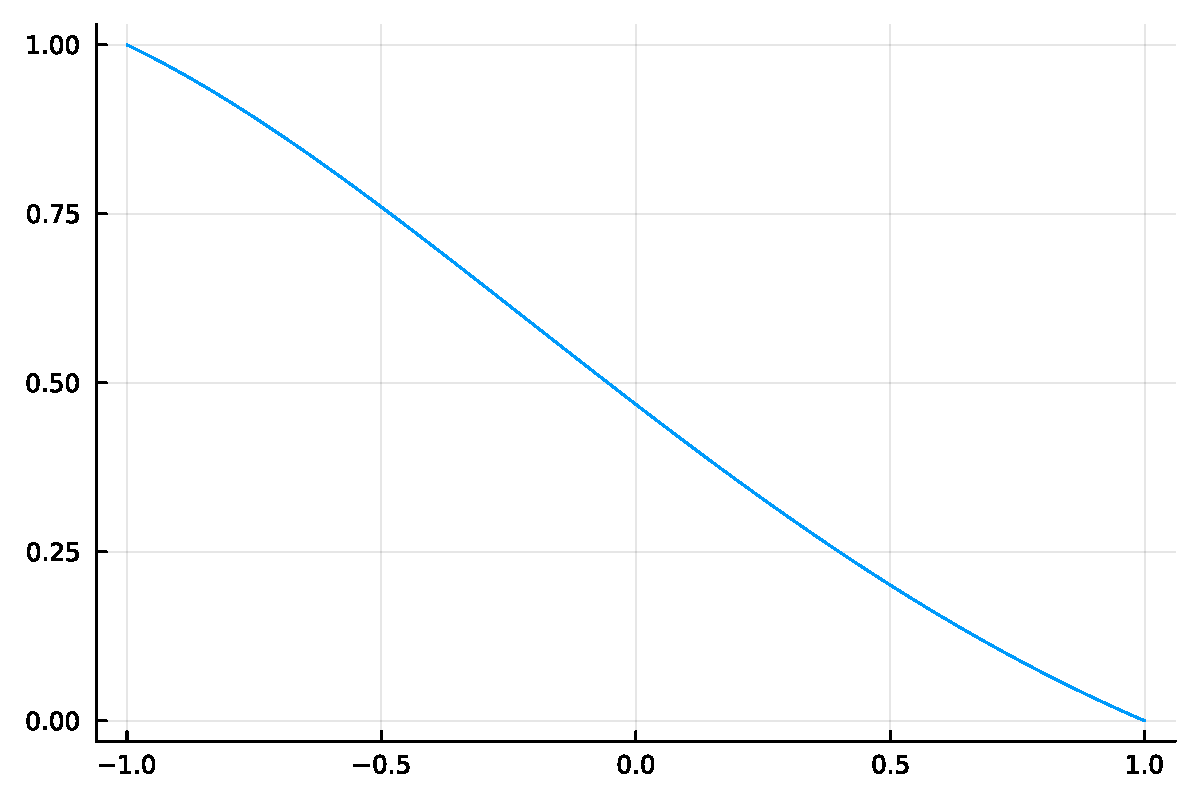
\includegraphics[width=\linewidth]{jl_dOthw0/OP_methods_41_1.pdf}

\subsubsection{Variable coefficients}
Consider the Airy ODE


\begin{align*}
u(-1) &= 1\\
u(1) &= 0\\
u''(x) - xu(x) &= 0
\end{align*}
to handle this, we need only use the Jacobi operator to represent multiplication by $x$:


\begin{lstlisting}
(*@\HLJLn{x}@*) (*@\HLJLoB{=}@*) (*@\HLJLnf{Fun}@*)(*@\HLJLp{()}@*)
(*@\HLJLn{X}@*) (*@\HLJLoB{=}@*) (*@\HLJLnf{Multiplication}@*)(*@\HLJLp{(}@*)(*@\HLJLn{x}@*)(*@\HLJLp{)}@*) (*@\HLJLoB{:}@*) (*@\HLJLnf{Chebyshev}@*)(*@\HLJLp{()}@*) (*@\HLJLoB{\ensuremath{\rightarrow}}@*) (*@\HLJLnf{Chebyshev}@*)(*@\HLJLp{()}@*)  (*@\HLJLcs{{\#}}@*) (*@\HLJLcs{transpose}@*) (*@\HLJLcs{of}@*) (*@\HLJLcs{the}@*) (*@\HLJLcs{Jacobi}@*) (*@\HLJLcs{operator}@*)
\end{lstlisting}

\begin{lstlisting}
ConcreteMultiplication : Chebyshev() (*@\ensuremath{\rightarrow}@*) Chebyshev()
 0.0  0.5   (*@\ensuremath{\cdot}@*)    (*@\ensuremath{\cdot}@*)    (*@\ensuremath{\cdot}@*)    (*@\ensuremath{\cdot}@*)    (*@\ensuremath{\cdot}@*)    (*@\ensuremath{\cdot}@*)    (*@\ensuremath{\cdot}@*)    (*@\ensuremath{\cdot}@*)   (*@\ensuremath{\cdot}@*)
 1.0  0.0  0.5   (*@\ensuremath{\cdot}@*)    (*@\ensuremath{\cdot}@*)    (*@\ensuremath{\cdot}@*)    (*@\ensuremath{\cdot}@*)    (*@\ensuremath{\cdot}@*)    (*@\ensuremath{\cdot}@*)    (*@\ensuremath{\cdot}@*)   (*@\ensuremath{\cdot}@*)
  (*@\ensuremath{\cdot}@*)   0.5  0.0  0.5   (*@\ensuremath{\cdot}@*)    (*@\ensuremath{\cdot}@*)    (*@\ensuremath{\cdot}@*)    (*@\ensuremath{\cdot}@*)    (*@\ensuremath{\cdot}@*)    (*@\ensuremath{\cdot}@*)   (*@\ensuremath{\cdot}@*)
  (*@\ensuremath{\cdot}@*)    (*@\ensuremath{\cdot}@*)   0.5  0.0  0.5   (*@\ensuremath{\cdot}@*)    (*@\ensuremath{\cdot}@*)    (*@\ensuremath{\cdot}@*)    (*@\ensuremath{\cdot}@*)    (*@\ensuremath{\cdot}@*)   (*@\ensuremath{\cdot}@*)
  (*@\ensuremath{\cdot}@*)    (*@\ensuremath{\cdot}@*)    (*@\ensuremath{\cdot}@*)   0.5  0.0  0.5   (*@\ensuremath{\cdot}@*)    (*@\ensuremath{\cdot}@*)    (*@\ensuremath{\cdot}@*)    (*@\ensuremath{\cdot}@*)   (*@\ensuremath{\cdot}@*)
  (*@\ensuremath{\cdot}@*)    (*@\ensuremath{\cdot}@*)    (*@\ensuremath{\cdot}@*)    (*@\ensuremath{\cdot}@*)   0.5  0.0  0.5   (*@\ensuremath{\cdot}@*)    (*@\ensuremath{\cdot}@*)    (*@\ensuremath{\cdot}@*)   (*@\ensuremath{\cdot}@*)
  (*@\ensuremath{\cdot}@*)    (*@\ensuremath{\cdot}@*)    (*@\ensuremath{\cdot}@*)    (*@\ensuremath{\cdot}@*)    (*@\ensuremath{\cdot}@*)   0.5  0.0  0.5   (*@\ensuremath{\cdot}@*)    (*@\ensuremath{\cdot}@*)   (*@\ensuremath{\cdot}@*)
  (*@\ensuremath{\cdot}@*)    (*@\ensuremath{\cdot}@*)    (*@\ensuremath{\cdot}@*)    (*@\ensuremath{\cdot}@*)    (*@\ensuremath{\cdot}@*)    (*@\ensuremath{\cdot}@*)   0.5  0.0  0.5   (*@\ensuremath{\cdot}@*)   (*@\ensuremath{\cdot}@*)
  (*@\ensuremath{\cdot}@*)    (*@\ensuremath{\cdot}@*)    (*@\ensuremath{\cdot}@*)    (*@\ensuremath{\cdot}@*)    (*@\ensuremath{\cdot}@*)    (*@\ensuremath{\cdot}@*)    (*@\ensuremath{\cdot}@*)   0.5  0.0  0.5  (*@\ensuremath{\cdot}@*)
  (*@\ensuremath{\cdot}@*)    (*@\ensuremath{\cdot}@*)    (*@\ensuremath{\cdot}@*)    (*@\ensuremath{\cdot}@*)    (*@\ensuremath{\cdot}@*)    (*@\ensuremath{\cdot}@*)    (*@\ensuremath{\cdot}@*)    (*@\ensuremath{\cdot}@*)   0.5  0.0  (*@\ensuremath{\ddots}@*)
  (*@\ensuremath{\cdot}@*)    (*@\ensuremath{\cdot}@*)    (*@\ensuremath{\cdot}@*)    (*@\ensuremath{\cdot}@*)    (*@\ensuremath{\cdot}@*)    (*@\ensuremath{\cdot}@*)    (*@\ensuremath{\cdot}@*)    (*@\ensuremath{\cdot}@*)    (*@\ensuremath{\cdot}@*)    (*@\ensuremath{\ddots}@*)   (*@\ensuremath{\ddots}@*)
\end{lstlisting}


We set up the system as follows:


\begin{lstlisting}
(*@\HLJLn{L}@*) (*@\HLJLoB{=}@*) (*@\HLJLp{[}@*)(*@\HLJLn{B\ensuremath{\_-}\ensuremath{\_1}}@*)(*@\HLJLp{;}@*)   (*@\HLJLcs{{\#}}@*) (*@\HLJLcs{u(-1)}@*)
     (*@\HLJLn{B\ensuremath{\_1}}@*) (*@\HLJLp{;}@*)   (*@\HLJLcs{{\#}}@*) (*@\HLJLcs{u(1)}@*)
     (*@\HLJLn{D\ensuremath{\_1}}@*)(*@\HLJLoB{*}@*)(*@\HLJLn{D\ensuremath{\_0}}@*) (*@\HLJLoB{-}@*) (*@\HLJLn{R{\_}U2}@*)(*@\HLJLoB{*}@*)(*@\HLJLn{R{\_}TU}@*)(*@\HLJLoB{*}@*)(*@\HLJLn{X}@*)(*@\HLJLp{]}@*)   (*@\HLJLcs{{\#}}@*) (*@\HLJLcs{u{\textquotesingle}{\textquotesingle}}@*) (*@\HLJLcs{-}@*) (*@\HLJLcs{x*u}@*)

(*@\HLJLn{u}@*) (*@\HLJLoB{=}@*) (*@\HLJLn{L}@*) (*@\HLJLoB{{\textbackslash}}@*) (*@\HLJLp{[}@*)(*@\HLJLnfB{1.0}@*)(*@\HLJLp{;}@*)(*@\HLJLnfB{0.0}@*)(*@\HLJLp{;}@*)(*@\HLJLnfB{0.0}@*)(*@\HLJLp{]}@*)
(*@\HLJLnf{plot}@*)(*@\HLJLp{(}@*)(*@\HLJLn{u}@*)(*@\HLJLp{;}@*) (*@\HLJLn{legend}@*)(*@\HLJLoB{=}@*)(*@\HLJLkc{false}@*)(*@\HLJLp{)}@*)
\end{lstlisting}

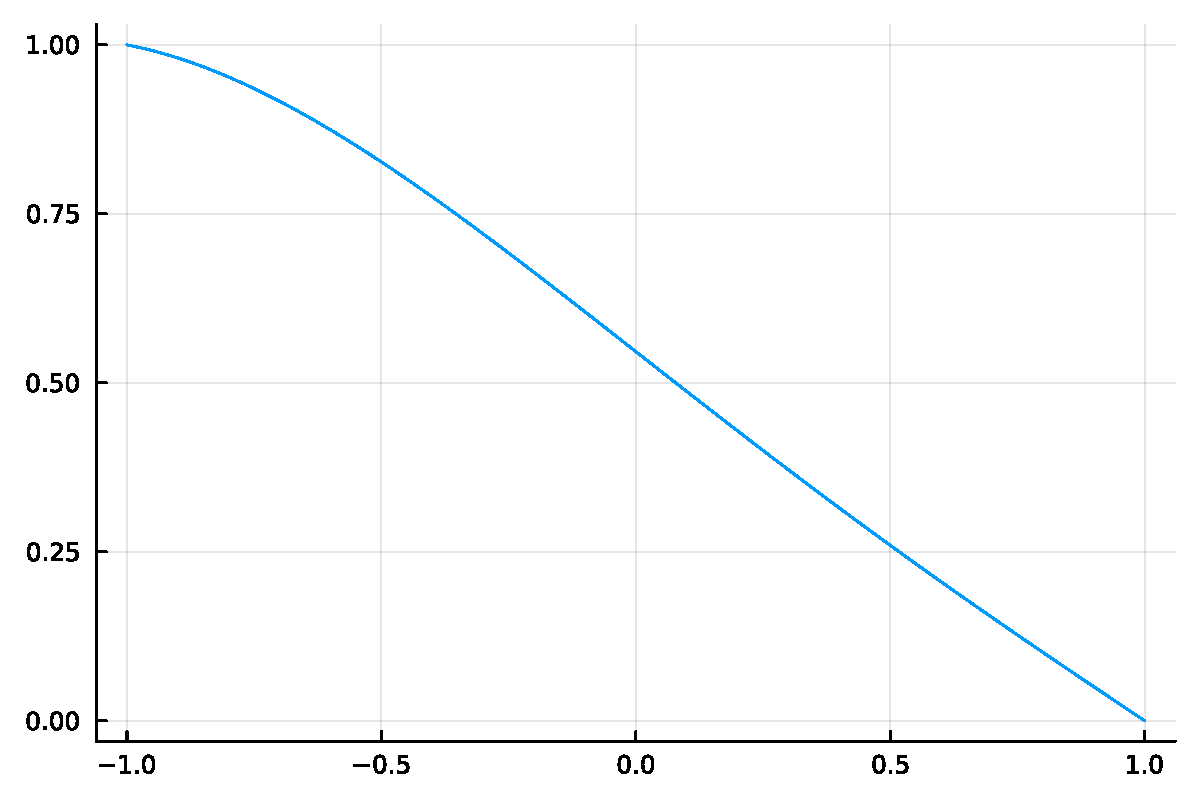
\includegraphics[width=\linewidth]{jl_dOthw0/OP_methods_43_1.pdf}

If we introduce a small parameter, that is, solve


\begin{align*}
u(-1) &= 1\\
u(1) &= 0\\
\epsilon u''(x) - xu(x) &= 0
\end{align*}
we can see it's pretty hard to compute solutions:


\begin{lstlisting}
(*@\HLJLn{\ensuremath{\varepsilon}}@*) (*@\HLJLoB{=}@*) (*@\HLJLnfB{1E-6}@*)
(*@\HLJLn{L}@*) (*@\HLJLoB{=}@*) (*@\HLJLp{[}@*)(*@\HLJLn{B\ensuremath{\_-}\ensuremath{\_1}}@*)(*@\HLJLp{;}@*)
     (*@\HLJLn{B\ensuremath{\_1}}@*) (*@\HLJLp{;}@*)
     (*@\HLJLn{\ensuremath{\varepsilon}}@*)(*@\HLJLoB{*}@*)(*@\HLJLn{D\ensuremath{\_1}}@*)(*@\HLJLoB{*}@*)(*@\HLJLn{D\ensuremath{\_0}}@*) (*@\HLJLoB{-}@*) (*@\HLJLn{R{\_}U2}@*)(*@\HLJLoB{*}@*)(*@\HLJLn{R{\_}TU}@*)(*@\HLJLoB{*}@*)(*@\HLJLn{X}@*)(*@\HLJLp{]}@*)

(*@\HLJLn{u}@*) (*@\HLJLoB{=}@*) (*@\HLJLn{L}@*) (*@\HLJLoB{{\textbackslash}}@*) (*@\HLJLp{[}@*)(*@\HLJLnfB{1.0}@*)(*@\HLJLp{;}@*)(*@\HLJLnfB{0.0}@*)(*@\HLJLp{;}@*)(*@\HLJLnfB{0.0}@*)(*@\HLJLp{]}@*)
(*@\HLJLnf{plot}@*)(*@\HLJLp{(}@*)(*@\HLJLn{u}@*)(*@\HLJLp{;}@*) (*@\HLJLn{legend}@*)(*@\HLJLoB{=}@*)(*@\HLJLkc{false}@*)(*@\HLJLp{)}@*)
\end{lstlisting}

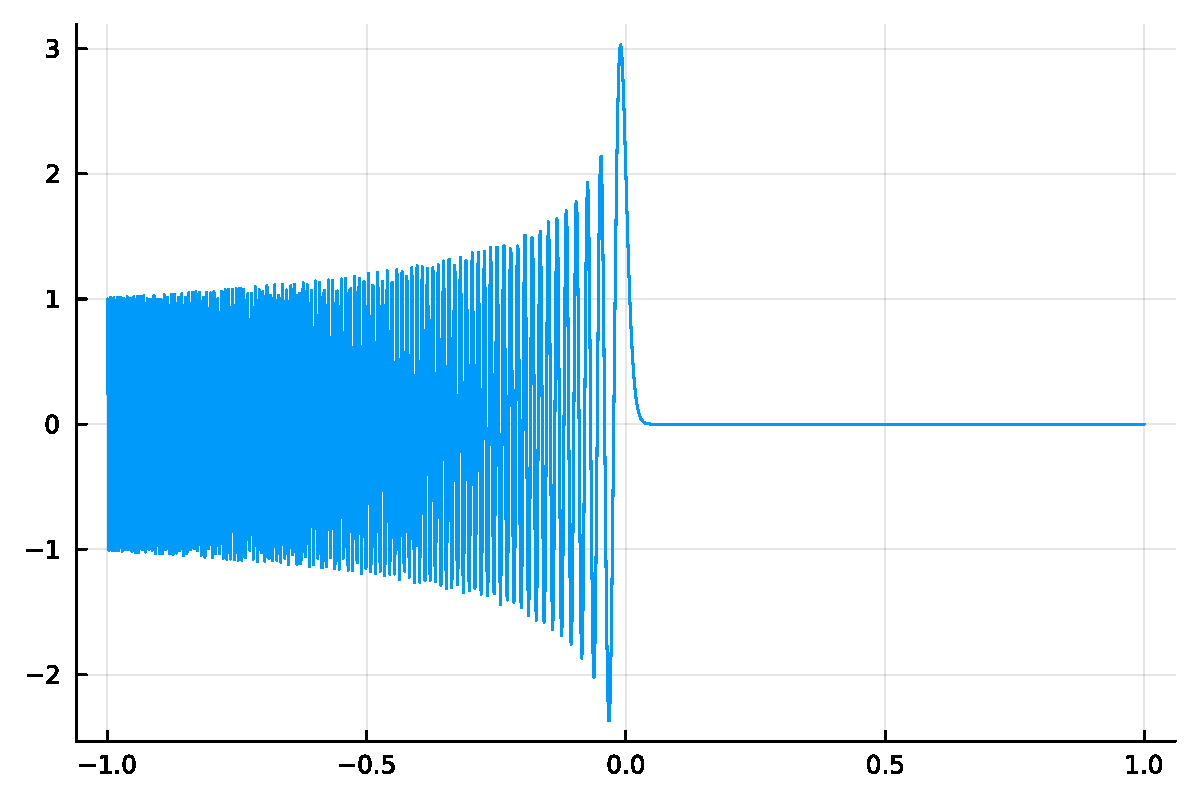
\includegraphics[width=\linewidth]{jl_dOthw0/OP_methods_44_1.pdf}

Because of the banded structure, this can be solved fast:


\begin{lstlisting}
(*@\HLJLn{\ensuremath{\varepsilon}}@*) (*@\HLJLoB{=}@*) (*@\HLJLnfB{1E-10}@*)
(*@\HLJLn{L}@*) (*@\HLJLoB{=}@*) (*@\HLJLp{[}@*)(*@\HLJLn{B\ensuremath{\_-}\ensuremath{\_1}}@*)(*@\HLJLp{;}@*)
     (*@\HLJLn{B\ensuremath{\_1}}@*) (*@\HLJLp{;}@*)
     (*@\HLJLn{\ensuremath{\varepsilon}}@*)(*@\HLJLoB{*}@*)(*@\HLJLn{D\ensuremath{\_1}}@*)(*@\HLJLoB{*}@*)(*@\HLJLn{D\ensuremath{\_0}}@*) (*@\HLJLoB{-}@*) (*@\HLJLn{R{\_}U2}@*)(*@\HLJLoB{*}@*)(*@\HLJLn{R{\_}TU}@*)(*@\HLJLoB{*}@*)(*@\HLJLn{X}@*)(*@\HLJLp{]}@*)

(*@\HLJLnd{@time}@*) (*@\HLJLn{u}@*) (*@\HLJLoB{=}@*) (*@\HLJLn{L}@*) (*@\HLJLoB{{\textbackslash}}@*) (*@\HLJLp{[}@*)(*@\HLJLnfB{1.0}@*)(*@\HLJLp{;}@*)(*@\HLJLnfB{0.0}@*)(*@\HLJLp{;}@*)(*@\HLJLnfB{0.0}@*)(*@\HLJLp{]}@*)
(*@\HLJLnd{@show}@*) (*@\HLJLnf{ncoefficients}@*)(*@\HLJLp{(}@*)(*@\HLJLn{u}@*)(*@\HLJLp{);}@*)
\end{lstlisting}

\begin{lstlisting}
1.796440 seconds (11.40 M allocations: 272.910 MiB, 4.22(*@{{\%}}@*) gc time)
ncoefficients(u) = 62496
\end{lstlisting}


To handle other variable coefficients, first consider a polynomial $p(x)$. If Multiplication by $x$ is represented by multiplying the coefficients by $J^\top$, then multiplication by $p$ is represented by multiplying the coefficients by $p(J^\top)$:


\begin{lstlisting}
(*@\HLJLn{M}@*) (*@\HLJLoB{=}@*) (*@\HLJLoB{-}@*)(*@\HLJLn{I}@*) (*@\HLJLoB{+}@*) (*@\HLJLn{X}@*) (*@\HLJLoB{+}@*) (*@\HLJLp{(}@*)(*@\HLJLn{X}@*)(*@\HLJLp{)}@*)(*@\HLJLoB{{\textasciicircum}}@*)(*@\HLJLni{2}@*)  (*@\HLJLcs{{\#}}@*) (*@\HLJLcs{represents}@*) (*@\HLJLcs{-1+x+x{\textasciicircum}2}@*)

(*@\HLJLn{\ensuremath{\varepsilon}}@*) (*@\HLJLoB{=}@*) (*@\HLJLnfB{1E-6}@*)
(*@\HLJLn{L}@*) (*@\HLJLoB{=}@*) (*@\HLJLp{[}@*)(*@\HLJLn{B\ensuremath{\_-}\ensuremath{\_1}}@*)(*@\HLJLp{;}@*)
     (*@\HLJLn{B\ensuremath{\_1}}@*) (*@\HLJLp{;}@*)
     (*@\HLJLn{\ensuremath{\varepsilon}}@*)(*@\HLJLoB{*}@*)(*@\HLJLn{D\ensuremath{\_1}}@*)(*@\HLJLoB{*}@*)(*@\HLJLn{D\ensuremath{\_0}}@*) (*@\HLJLoB{-}@*) (*@\HLJLn{R{\_}U2}@*)(*@\HLJLoB{*}@*)(*@\HLJLn{R{\_}TU}@*)(*@\HLJLoB{*}@*)(*@\HLJLn{M}@*)(*@\HLJLp{]}@*)

(*@\HLJLnd{@time}@*) (*@\HLJLn{u}@*) (*@\HLJLoB{=}@*) (*@\HLJLn{L}@*) (*@\HLJLoB{{\textbackslash}}@*) (*@\HLJLp{[}@*)(*@\HLJLnfB{1.0}@*)(*@\HLJLp{;}@*)(*@\HLJLnfB{0.0}@*)(*@\HLJLp{;}@*)(*@\HLJLnfB{0.0}@*)(*@\HLJLp{]}@*)

(*@\HLJLnd{@show}@*) (*@\HLJLn{\ensuremath{\varepsilon}}@*)(*@\HLJLoB{*}@*)(*@\HLJLn{u}@*)(*@\HLJLoB{{\textquotesingle}{\textquotesingle}}@*)(*@\HLJLp{(}@*)(*@\HLJLnfB{0.1}@*)(*@\HLJLp{)}@*) (*@\HLJLoB{-}@*) (*@\HLJLp{(}@*)(*@\HLJLoB{-}@*)(*@\HLJLni{1}@*)(*@\HLJLoB{+}@*)(*@\HLJLnfB{0.1}@*)(*@\HLJLoB{+}@*)(*@\HLJLnfB{0.1}@*)(*@\HLJLoB{{\textasciicircum}}@*)(*@\HLJLni{2}@*)(*@\HLJLp{)}@*)(*@\HLJLoB{*}@*)(*@\HLJLnf{u}@*)(*@\HLJLp{(}@*)(*@\HLJLnfB{0.1}@*)(*@\HLJLp{)}@*)
(*@\HLJLnf{plot}@*)(*@\HLJLp{(}@*)(*@\HLJLn{u}@*)(*@\HLJLp{)}@*)
\end{lstlisting}

\begin{lstlisting}
0.055510 seconds (245.78 k allocations: 6.347 MiB)
(*@\ensuremath{\varepsilon}@*) * ((u(*@{{\textquotesingle}}@*))(*@{{\textquotesingle}}@*))(0.1) - (-1 + 0.1 + 0.1 (*@{{\textasciicircum}}@*) 2) * u(0.1) = -1.469657728847551e-14
\end{lstlisting}

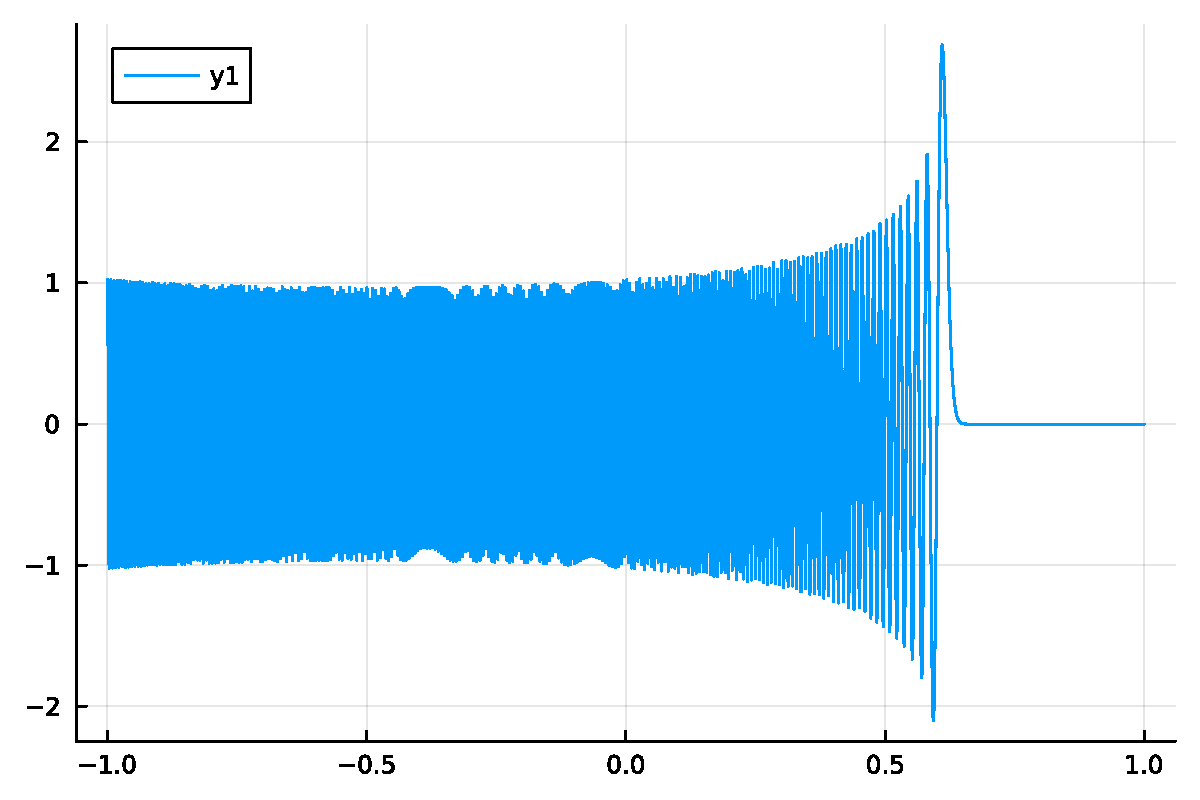
\includegraphics[width=\linewidth]{jl_dOthw0/OP_methods_46_1.pdf}

For other smooth functions, we first approximate in a polynomial basis,  and without loss of generality we use Chebyshev T basis. For example, consider


\begin{align*}
u(-1) &= 1\\
u(1) &= 0\\
\epsilon u''(x) - {\rm e}^x u(x) &= 0
\end{align*}
where

\[
{\rm e}^x  \approx p(x) = \sum_{k=0}^{m-1} p_k T_k(x)
\]
Evaluating at a point $x$, recall Clenshaw's algorithm:


\begin{align*}
\gamma_{n-1} &= 2p_{n-1} \\
\gamma_{n-2} &= 2p_{n-2} + 2x \gamma_{n-1} \\
\gamma_{n-3} &= 2 p_{n-3} + 2x \gamma_{n-2} - \gamma_{n-1} \\
& \vdots \\
\gamma_1 &= p_1 + x \gamma_2 - {1 \over 2} \gamma_3 \\
p(x) = \gamma_0 &= p_0 + x \gamma_1 - {1 \over 2} \gamma_2
\end{align*}
If multiplication by $x$ becomes $J^\top$, then multiplication by $p(x)$ becomes $p(J^\top)$, and hence we calculate:


\begin{align*}
\Gamma_{n-1} &= 2p_{n-1}I \\
\Gamma_{n-2} &= 2p_{n-2}I + 2J^\top \Gamma_{n-1} \\
\Gamma_{n-3} &= 2 p_{n-3}I + 2J^\top \Gamma_{n-2} - \Gamma_{n-1} \\
& \vdots \\
\Gamma_1 &= p_1I + J^\top \Gamma_2 - {1 \over 2} \Gamma_3 \\
p(J^\top) = \Gamma_0 &= p_0 + J^\top \Gamma_1 - {1 \over 2} \Gamma_2
\end{align*}
Here is an example:


\begin{lstlisting}
(*@\HLJLn{p}@*) (*@\HLJLoB{=}@*) (*@\HLJLnf{Fun}@*)(*@\HLJLp{(}@*)(*@\HLJLn{exp}@*)(*@\HLJLp{,}@*) (*@\HLJLnf{Chebyshev}@*)(*@\HLJLp{())}@*) (*@\HLJLcs{{\#}}@*) (*@\HLJLcs{polynomial}@*) (*@\HLJLcs{approximation}@*) (*@\HLJLcs{to}@*) (*@\HLJLcs{exp(x)}@*)
(*@\HLJLn{M}@*) (*@\HLJLoB{=}@*) (*@\HLJLnf{Multiplication}@*)(*@\HLJLp{(}@*)(*@\HLJLn{p}@*)(*@\HLJLp{)}@*) (*@\HLJLoB{:}@*) (*@\HLJLnf{Chebyshev}@*)(*@\HLJLp{()}@*) (*@\HLJLcs{{\#}}@*) (*@\HLJLcs{constructed}@*) (*@\HLJLcs{using}@*) (*@\HLJLcs{Clenshaw:}@*)

(*@\HLJLn{\ensuremath{\varepsilon}}@*) (*@\HLJLoB{=}@*) (*@\HLJLnfB{1E-6}@*)
(*@\HLJLn{L}@*) (*@\HLJLoB{=}@*) (*@\HLJLp{[}@*)(*@\HLJLn{B\ensuremath{\_-}\ensuremath{\_1}}@*)(*@\HLJLp{;}@*)
     (*@\HLJLn{B\ensuremath{\_1}}@*) (*@\HLJLp{;}@*)
     (*@\HLJLn{\ensuremath{\varepsilon}}@*)(*@\HLJLoB{*}@*)(*@\HLJLn{D\ensuremath{\_1}}@*)(*@\HLJLoB{*}@*)(*@\HLJLn{D\ensuremath{\_0}}@*) (*@\HLJLoB{+}@*) (*@\HLJLn{R{\_}U2}@*)(*@\HLJLoB{*}@*)(*@\HLJLn{R{\_}TU}@*)(*@\HLJLoB{*}@*)(*@\HLJLn{M}@*)(*@\HLJLp{]}@*)

(*@\HLJLnd{@time}@*) (*@\HLJLn{u}@*) (*@\HLJLoB{=}@*) (*@\HLJLn{L}@*) (*@\HLJLoB{{\textbackslash}}@*) (*@\HLJLp{[}@*)(*@\HLJLnfB{1.0}@*)(*@\HLJLp{;}@*)(*@\HLJLnfB{0.0}@*)(*@\HLJLp{;}@*)(*@\HLJLnfB{0.0}@*)(*@\HLJLp{]}@*)

(*@\HLJLnd{@show}@*) (*@\HLJLn{\ensuremath{\varepsilon}}@*)(*@\HLJLoB{*}@*)(*@\HLJLn{u}@*)(*@\HLJLoB{{\textquotesingle}{\textquotesingle}}@*)(*@\HLJLp{(}@*)(*@\HLJLnfB{0.1}@*)(*@\HLJLp{)}@*) (*@\HLJLoB{+}@*) (*@\HLJLnf{exp}@*)(*@\HLJLp{(}@*)(*@\HLJLnfB{0.1}@*)(*@\HLJLp{)}@*)(*@\HLJLoB{*}@*)(*@\HLJLnf{u}@*)(*@\HLJLp{(}@*)(*@\HLJLnfB{0.1}@*)(*@\HLJLp{)}@*)
(*@\HLJLnf{plot}@*)(*@\HLJLp{(}@*)(*@\HLJLn{u}@*)(*@\HLJLp{)}@*)
\end{lstlisting}

\begin{lstlisting}
0.168037 seconds (908.09 k allocations: 20.127 MiB)
(*@\ensuremath{\varepsilon}@*) * ((u(*@{{\textquotesingle}}@*))(*@{{\textquotesingle}}@*))(0.1) + exp(0.1) * u(0.1) = 5.10702591327572e-15
\end{lstlisting}

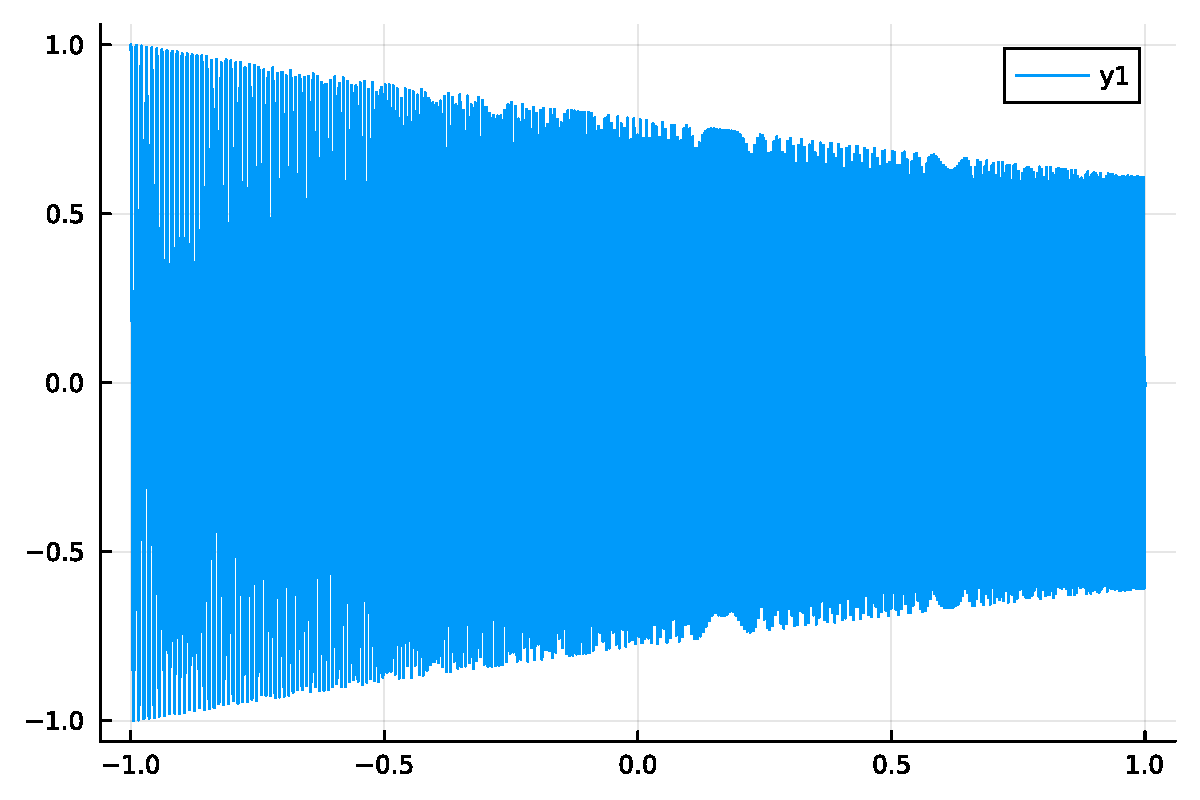
\includegraphics[width=\linewidth]{jl_dOthw0/OP_methods_47_1.pdf}

\section{Differential equations satisfied by orthogonal polynomials}
This lecture we do the following:

\begin{itemize}
\item[1. ] Differential equations for orthogonal polynomials

\begin{itemize}
\item Sturm\ensuremath{\endash}Liouville equations


\item Weighted differentiation for ultraspherical polynomials


\item Differential equation for ultraspherical polynomials

\end{itemize}

\item[2. ] Application: Eigenstates of Schrödinger operators with quadratic potentials

\end{itemize}
The three classical weights are (Hermite) $w(x) = {\rm e}^{-x^2}$, (Laguerre) $w_\alpha(x) = x^\alpha {\rm e}^{-x}$ and (Jacobi) $w_{\alpha,\beta}(x) = (1-x)^\alpha (1+x)^\beta$. Note all weights form a simple hierarchy: when differentiated, they give a linear polynomial times the previous weight in the hierarchy.  For Hermite,

\[
{{\rm d} \over {\rm d}x} w(x) = -2x w(x)
\]
for Laguerre,

\[
{{\rm d} \over {\rm d}x} w^{(\alpha)}(x) = (\alpha  - x) w^{(\alpha-1)}(x)
\]
and for Jacobi

\[
{{\rm d} \over {\rm d}x} w^{(\alpha,\beta)}(x) = (\beta(1-x) - \alpha(1+x)) w^{(\alpha-1,\beta-1)}(x)
\]
These relationships  lead to simple differential equations that have the classical orthogonal polynomials as eigenfunctions.

\subsubsection{Sturm\ensuremath{\endash}Liouville operator}
We first consider a simple class of operators that are self-adjoint:

\textbf{Proposition (Sturm\ensuremath{\endash}Liouville self-adjointness)} Consider the weighted inner product

\[
\langle f,g\rangle_w = \int_a^b f(x) g(x) w(x) {\rm d}x
\]
then for any continuously differentiable function $q(x)$ satisfying $q(a) = q(b) = 0$, the operator

\[
Lu = {1 \over w(x)} {{\rm d} \over {\rm d}x}\left[ q(x) {{\rm d} u\over {\rm d}x} \right]
\]
is self-adjoint in the sense

\[
\langle L f,g\rangle_w = \langle f, Lg\rangle_w
\]
\textbf{Proof} Simple integration by parts argument:


\begin{align*}
\langle L f,g\rangle_w &= \int_a^b {{\rm d} \over {\rm d}x}\left[ q(x) {{\rm d} u\over {\rm d}x}\right]  g(x){\rm d}x 
=  -\int_a^b q(x) {{\rm d} u\over {\rm d}x}    {{\rm d} g\over {\rm d}x} {\rm d}x =  \int_a^b   u(x)  {{\rm d} \over {\rm d}x} \left[ q(x) {{\rm d} g\over {\rm d}x}\right] {\rm d}x 
=
 \int_a^b   u(x)  {1 \over w(x)} {{\rm d} \over {\rm d}x}\left[q(x) {{\rm d} g\over {\rm d}x}\right] w(x) {\rm d}x = \langle f, Lg\rangle_w
 \end{align*}
\[
\blacksquare
\]
We claim that the classical orthogonal polynomials are eigenfunctions of a Sturm\ensuremath{\endash}Liouville problem, that is, in each case there exists a $q(x)$ so that

\[
L p_n(x) = \lambda_n p_n(x)
\]
where $\lambda_n$ is the (real) eigenvalue. We will derive this for the ultraspherical polynomials.

\subsubsection{Weighted differentiation for ultraspherical polynomials}
We have already seen that Chebyshev and ultraspherical polynomials have simple expressions for derivatives where we decrement the degree and increment the parameter:


\begin{align*}
{{\rm d} \over {\rm d}x } T_n(x) & = n U_{n-1}(x) = n C_{n-1}^{(1)}(x) \\
{{\rm d} \over {\rm d}x } C_n^{(\lambda)}(x) &= 2 \lambda C_{n-1}^{(\lambda+1)}(x)
\end{align*}
In this section, we see that differentiating the weighted polynomials actually decrements the parameter and increments the degree:

\textbf{Proposition (weighted differentiation)}


\begin{align*}
{{\rm d} \over {\rm d}x }[\sqrt{1-x^2} U_n(x)] &= - {n+1 \over \sqrt{1-x^2}} T_{n+1}(x) \\
{{\rm d} \over {\rm d}x }[(1-x^2)^{\lambda-{1 \over 2}} C_n^{(\lambda)}(x)] & = -{(n+1) (n+2 \lambda-1) \over 2 (\lambda-1) }  (1-x^2)^{\lambda - {3 \over 2}} C_{n+1}^{(\lambda-1)}(x)
\end{align*}
\textbf{Proof} We show the first result by showing that the left-hand side is orthogonal to all  polynomials of degree less than $n+1$ by integration by parts:

\[
\langle  \sqrt{1-x^2} {{\rm d} \over {\rm d}x }[\sqrt{1-x^2} U_n(x)], p_m(x)\rangle_{\rm T} = -\int_{-1}^1 \sqrt{1-x^2} U_n(x) p_m' {\rm d}x =0
\]
Note that

\[
\sqrt{1-x^2} {{\rm d} \over {\rm d}x } \sqrt{1-x^2} f(x) = (1-x^2) f'(x) - x f(x)
\]
Thus we just have to verify the constant in front:

\[
\sqrt{1-x^2} {{\rm d} \over {\rm d}x }[\sqrt{1-x^2} U_n(x) = (-n -1) 2^n x^{n+1}
\]
The other ultraspherical polynomial follow similarly. $\blacksquare$

\subsubsection{Eigenvalue equation for Ultraspherical polynomials}
Note that differentiating increments the parameter and decrements the degree while weighted differentiation decrements the parameter and increments the degree. Therefore combining them brings us back to where we started.

In the case of Chebyshev polynomials, this gives us a Sturm\ensuremath{\endash}Liouville equation:

\[
\sqrt{1-x^2} {{\rm d} \over {\rm d}x} \sqrt{1-x^2} {{\rm d} T_n \over {\rm d}x} =
n \sqrt{1-x^2} {{\rm d} \over {\rm d}x} \sqrt{1-x^2} U_{n-1}(x) = -n^2 T_n(x)
\]
Note that the chain rule gives us a simple expression as

\[
(1-x^2) {{\rm d}^2 T_n \over {\rm d}x^2} -x {{\rm d} T_n \over {\rm d}x} = -n^2 T_n(x)
\]
Similarly,

\[
(1-x^2)^{{1 \over 2} - \lambda} {{\rm d} \over {\rm d}x}(1-x^2)^{\lambda + {1 \over 2}} {{\rm d} C_n^{(\lambda)} \over {\rm d}x} = -n (n+2 \lambda) C_n^{(\lambda)}(x)
\]
or in other words,

\[
(1-x^2) {{\rm d}^2 C_n^{(\lambda)} \over {\rm d}x^2} - (2\lambda+1) x {{\rm d} C_n^{(\lambda)} \over {\rm d}x}  = -{n (n+2 \lambda) \over 2\lambda}C_n^{(\lambda)}(x)
\]

\begin{lstlisting}

\end{lstlisting}


\begin{lstlisting}

\end{lstlisting}


definition three term recurrences Clenshaw examples Jacobi matrix vector space roots of OPs are eigenvalues of Jacobi matrix roots of OPs, quadrature, coefficients, interpolation, transforms Gram Schmidt approximation by expansion in OPs derivatives conversion Multiplication function value space and coefficient space The monomial basis Chebyshev polynomials The Chebyshev Fourier connection Differential equations PDE example

\begin{itemize}
\item[1.  ] Runge phenomenon


\item[2.  ] Chebyshev-Fourier connection


\item[3.  ] Orthogonal polynomials


\item[4.  ] Coefficient space and function value space


\item[5.  ] Boundary-value problems


\item[6.  ] Ultraspherical method, collocation method, finite difference method, Galerkin and finite element method


\item[7.  ] Vector spaces


\item[8.  ] Fourier-orthogonality connection


\item[9.  ] Instability of monomial basis

\end{itemize}


\end{document}
